\documentclass[11pt]{article}
\usepackage[margin=2.4cm]{geometry}
\usepackage{amsmath,amssymb,mathtools,amsthm}
\usepackage{enumitem}
\usepackage{booktabs,array}
\usepackage{tikz}
\usetikzlibrary{arrows.meta,positioning,calc}
\usepackage{float}
\usepackage{verbatim}
\usepackage[colorlinks=true,linkcolor=blue!55!black,citecolor=blue!55!black,urlcolor=blue!55!black]{hyperref}
\usepackage{cleveref}
\usepackage{fontspec}
% Noto Serif CJK KR ships no italic; AutoFakeSlant supplies one so \emph does not
% silently fall back to upright. The linebreak locale enables Korean line breaking,
% without which every Korean paragraph overfills.
\setmainfont[AutoFakeSlant=0.2]{Noto Serif CJK KR}
\setsansfont{Noto Sans CJK KR}
\XeTeXlinebreaklocale "ko"
\XeTeXlinebreakskip = 0pt plus 1pt
\tolerance=2500
\emergencystretch=3em

\theoremstyle{plain}
\newtheorem{theorem}{Theorem}[section]
\newtheorem{lemma}[theorem]{Lemma}
\newtheorem{proposition}[theorem]{Proposition}
\newtheorem{corollary}[theorem]{Corollary}
\theoremstyle{definition}
\newtheorem{definition}[theorem]{Definition}
\newtheorem{assumption}[theorem]{Assumption}
\newtheorem{example}[theorem]{Example}
\theoremstyle{remark}
\newtheorem{remark}[theorem]{Remark}

% One glyph per object: m is the action dimension only; mass is \mass; planar and spatial
% inertia are both \inertia; the learned certificate is \Vhat everywhere.
\newcommand{\R}{\mathbb{R}}
\newcommand{\E}{\mathbb{E}}
\newcommand{\Prob}{\mathbb{P}}
\DeclarePairedDelimiter{\norm}{\lVert}{\rVert}
\DeclarePairedDelimiter{\abs}{\lvert}{\rvert}
\newcommand{\inner}[2]{\langle #1,\,#2\rangle}
\newcommand{\calX}{\mathcal{X}}
\newcommand{\calU}{\mathcal{U}}
\newcommand{\calA}{\mathcal{A}}
\newcommand{\calC}{\mathcal{C}}
\newcommand{\calO}{\mathcal{O}}
\newcommand{\calK}{\mathcal{K}}
\newcommand{\calS}{\mathcal{S}}
\newcommand{\calF}{\mathcal{F}}
\newcommand{\calT}{\mathcal{T}}
\newcommand{\calD}{\mathcal{D}}
\newcommand{\calB}{\mathcal{B}}
\newcommand{\calM}{\mathcal{M}}
\newcommand{\calQ}{\mathcal{Q}}
\newcommand{\SO}{\mathrm{SO}}
\newcommand{\Vhp}[1]{V^{h,#1}}
\newcommand{\Vhpi}{\Vhp{\pi}}
\newcommand{\Vhat}{\widehat V}
\newcommand{\hV}{\Vhat}
\newcommand{\mass}{\mathsf m}
\newcommand{\inertia}{\mathcal I}
\newcommand{\tV}{\tilde{V}}
\newcommand{\Lg}{L_g}
\newcommand{\Lf}{L_f}
\newcommand{\grad}{\nabla}
\newcommand{\Hu}{H_u}
\newcommand{\viol}{\mathrm{viol}}
\newcommand{\sgn}{\operatorname{sgn}}
\newcommand{\eqdef}{:=}

\title{\textbf{JT-PNCBF Theory (consolidated)}\\[2mm]
{\large Part I: Underactuated Joint Training \quad\textbullet\quad Part II: Double Integrator, Self-Conditioning}}
\author{JT-PNCBF project}
\date{}

\begin{document}
\maketitle

\begin{abstract}
We ask whether an observation-conditioned policy neural CBF can be trained jointly with the
policy, through a hard projection filter and without any external shield, on an underactuated
quadrotor. Part~I treats that question. A hand-designed position-only hazard has thrust
relative degree $2$ and torque relative degree $4$; the policy value $\Vhpi=\sup_{t\ge0}h$
collapses both to one, but the collapse does not by itself produce input authority. We identify
where it fails: on any open set where the future maximum is attained at the present state, the
exact value equals the hazard, so a position-only hazard hands the value a gradient with no
velocity and no rate component, and both input channels vanish there. That set has positive
measure, so the failure is a property of the exact object and no amount of training removes it.
Adding a velocity lead restores the thrust channel on that set up to a null subset; adding a
rate term restores the torque channel. Whether the degeneracy is null on the whole operating
region remains open. We then record what the deployed realization does and does not inherit:
the finite-candidate filter is a projection only up to action dimension two, so at per-rotor
dimension four it is a selection, discontinuous across ties and gradient-free wherever a box
vertex wins; a single-scalar dual solve is exact and continuous in every dimension.
Sampled-data statements bound the inter-sample excursion and show why a finer control period
helps sub-quadratically. Part~II collects the double-integrator results on self-conditioning:
the separation of the safety channel from policy optimization, the degeneracy of
self-referential evaluation, a fully discrete margin theorem with a measurable error budget,
and the maneuver-family barrier that realizes the safety guarantees with no learned object in
the safety channel. Every empirical figure carries its seed basis, pool, and device; retracted
hypotheses are kept as retractions.
\end{abstract}

\tableofcontents
\newpage

\part{Underactuated joint training}
\section{Overview}\label{sec:overview}

\begin{figure}[H]
\centering
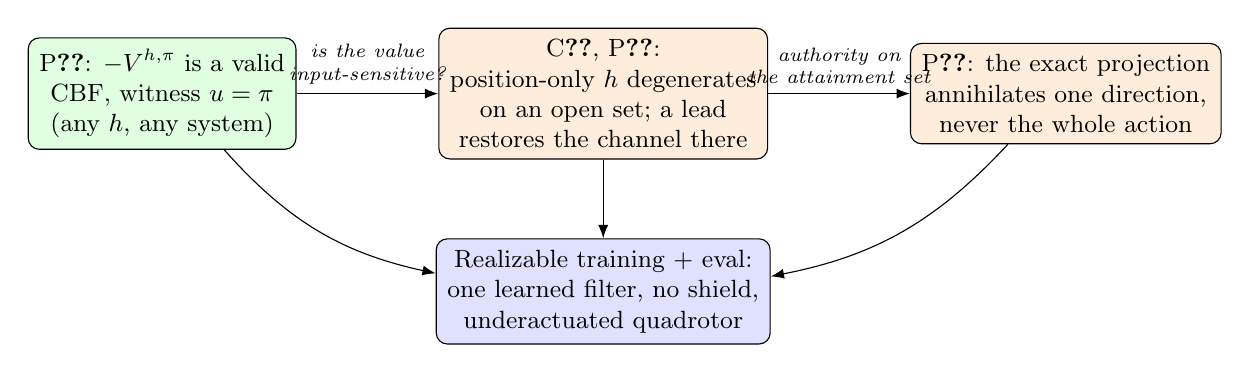
\begin{tikzpicture}[
  >=Latex, node distance=6mm,
  box/.style={draw, rounded corners, align=center, font=\small, inner sep=4pt, minimum height=9mm},
  uncond/.style={box, fill=green!12},
  cond/.style={box, fill=orange!14},
  goal/.style={box, fill=blue!12},
  lab/.style={font=\scriptsize\itshape, align=center}
]
\node[uncond] (val) {P\ref{prop:validity}: $-\Vhpi$ is a valid\\ CBF, witness $u=\pi$\\ (any $h$, any system)};
\node[cond, right=18mm of val] (ctrl) {C\ref{cor:degen-pos}, P\ref{prop:lead}:\\ position-only $h$ degenerates\\ on an open set; a lead\\ restores the channel there};
\node[cond, right=18mm of ctrl] (jt) {P\ref{prop:jt}: the exact projection\\ annihilates one direction,\\ never the whole action};
\node[goal, below=10mm of ctrl] (impl) {Realizable training + eval:\\ one learned filter, no shield,\\ underactuated quadrotor};

\draw[->] (val) -- node[lab, above]{is the value\\ input-sensitive?} (ctrl);
\draw[->] (ctrl) -- node[lab, above]{authority on\\ the attainment set} (jt);
\draw[->] (val) to[bend right=18] (impl);
\draw[->] (ctrl) -- (impl);
\draw[->] (jt) to[bend left=18] (impl);
\end{tikzpicture}
\caption{Dependency chain of the controllability foundation for joint training.}
\label{fig:overview}
\end{figure}

\textbf{직관 (이 문서가 세우는 것).}
목표는 shield 같은 외부 dynamics 장치 없이, 학습된 observation-conditioned PNCBF \emph{하나로}
underactuated 계에서 안전과 성능을 동시에 확보하고, 그 확보를 value와 policy의
\emph{joint training}으로 달성하는 것이다. hand-designed CBF $h$는 underactuated 계에서 높은 vector relative
degree를 가져 first order로 입력을 제약하지 못한다(\cref{sec:relhu}). PNCBF는 policy value
function $\Vhpi=\sup_{t\ge0}h(x_t^\pi)$를 학습하여 이 relative degree를 $1$로 낮추지만
(\cref{prop:validity}), underactuation 하에서 $\Lg\Vhpi$가 특정 상태에서 소멸할 수 있다. 이 소멸
집합의 measure가 joint training의 성패를 가른다. \cref{cor:degen-pos}은 position-only $h$ 하에서
이 집합이 양의 측도를 가짐을 보이고, \cref{prop:lead}은 최소 증강이 그 집합 위에서 각 채널을
어떻게 되살리는지를 준다. 전역 판정은 열려 있다(\cref{rem:global-open}). 결과는 planar($\SO(2)$)와
spatial($\SO(3)$) quadrotor를 공통 구조 가정의 두 실현으로 함께 다룬다(\cref{sec:setup}).

\section{Setup and realizable assumptions}\label{sec:setup}

\begin{definition}[Control-affine underactuated navigation system]\label{def:sys}
A system on state $x=(p,R,v,\omega)\in\calX$ with
position $p\in\R^d$ ($d\in\{2,3\}$),
attitude $R\in\SO(d)$,
linear velocity $v\in\R^d$,
body angular velocity $\omega\in\R^{d(d-1)/2}$,
and control $u=(f_{\mathrm{thr}},\tau)\in\calU\subset\R^{m}$
(scalar thrust $f_{\mathrm{thr}}\in\R$ along a fixed body axis $e\in\R^d$, torque
$\tau\in\R^{d(d-1)/2}$, $m=1+d(d-1)/2$), is
\begin{equation}
\dot p = v,\qquad
\dot v = \tfrac{1}{\mass}\,f_{\mathrm{thr}}\,R e - g\,e_g,\qquad
\dot R = R\,\widehat{\omega},\qquad
\dot\omega = \inertia^{-1}\!\big(\tau-\omega\times\inertia\omega\big),
\end{equation}
with mass $\mass>0$, gravity $g\ge0$ along fixed $e_g$, inertia $\inertia\succ0$, and
$\widehat{(\cdot)}$ the $\R^{d(d-1)/2}\!\to\mathfrak{so}(d)$ hat map. Write it as
$\dot x=f(x)+\sum_{j=1}^m g_j(x)u_j$.
\end{definition}

\begin{definition}[Underactuation structure]\label{def:under}
System \cref{def:sys} is \textbf{\emph{position-underactuated}}: the only control entering
$\dot v$ is the scalar thrust $f_{\mathrm{thr}}$, and it enters solely through the
attitude-steered direction $Re$; the torque $\tau$ enters $\dot\omega$ only. Equivalently,
\begin{equation}
\grad_p g_j \equiv 0,\qquad
g_{f_{\mathrm{thr}}}\ \text{acts on }\dot v\text{ as }\tfrac1{\mass}Re,\qquad
g_{\tau}\ \text{acts on }\dot\omega\text{ only.}
\end{equation}
\end{definition}

\begin{assumption}[Realizable standing assumptions]\label{asm:standing}
The following hold throughout; each is checkable in the training/eval code.
\begin{itemize}[leftmargin=1.8em]
  \item[\textbf{(A1)}] \textbf{Fixed feasible nominal policy.} $\pi:\calX\times\calO\to\calU$ is a fixed, $\calU$-valued, locally Lipschitz nominal policy (the deployed LQR/PD-tracking law), so $u=\pi(x,o)$ is admissible at every $x$.
  \item[\textbf{(A2)}] \textbf{Observation encoding.} $o\in\calO$ is the runtime Top-$K$ obstacle encoding; on each fixed $o$ the results below hold verbatim, matching the observation-conditioned training protocol.
  \item[\textbf{(A3)}] \textbf{Compact operating region.} States are confined to a compact $\calX_0\subset\calX$ (arena bound and the velocity clamp $\norm{v}\le v_{\max}$ enforced by the simulator), on which $f,g,h$ are $C^2$.
  \item[\textbf{(A4)}] \textbf{Bounded input box.} $\calU=[\,\underline f,\overline f\,]\times\prod_i[\,-\overline\tau_i,\overline\tau_i\,]$ is a nonempty box; the HardNet projection is the box-aware closed form on $\calU$.
  \item[\textbf{(A5)}] \textbf{Design freedom in $h$.} The avoid-set generator $h:\calX\times\calO\to\R$ ($\calA=\{h>0\}$) is a design object, chosen as simple as possible subject to realizing the control we require; it need not be position-only.
\end{itemize}
\end{assumption}

\textbf{해석 (가정의 실현성).}
(A1)은 PNCBF validity의 원 가정이며 코드의 고정 nominal policy가 그대로 만족한다. (A3)의 컴팩트성과
속도 clamp는 simulator의 \texttt{wrap\_state}가 강제하는 실제 조건이고, $C^2$는 $h$를 매끄럽게
설계함으로써 확보된다(A5). (A4)는 box-aware HardNet이 요구하는 그대로다.
underactuation(\cref{def:under})은 quadrotor 물리 그 자체이며 새 가정이 아니다.

\section{The vector relative degree of a hand-designed \texorpdfstring{$h$}{h}}\label{sec:relhu}

\textbf{직관 (왜 $h$ 자체로는 부족한가).}
control-affine 계에서 decoupling은 Lie derivative $[\Hu(x)]_{ij}=L_{g_j}\Lf^{\,r_i-1}h_i(x)$의
rank로 결정된다. 이 절은 position-based $h$에 대해 $\Hu(x)$를 명시적으로 계산하여 두 입력 채널의
relative degree를 확정하고, thrust 항이 소멸하는 집합이 null임을 보인다 --- 즉 어려움의 원천은 그
집합이 아니라 다음 절이 구성하는 열린 집합이다.

\begin{definition}[Decoupling matrix]\label{def:hu}
For outputs $y=(h_1,\dots,h_p)$ with vector relative degree $(r_1,\dots,r_p)$ at $x$,
\begin{equation}
\Hu(x)\in\R^{p\times m},\qquad [\Hu(x)]_{ij}\eqdef L_{g_j}\Lf^{\,r_i-1}h_i(x),
\end{equation}
the control-affine generalization of the LTI Markov-parameter matrix $[\,c_iA^{r_i-1}B_j\,]$.
\end{definition}

\begin{proposition}[Relative degree of a position-only hazard]\label{prop:relh}
Let $h(x)=\phi(p)$ with $\phi\in C^4$ and $\grad\phi\neq0$ on $\calX_0$, under
\cref{def:sys,def:under}. Then, scope: exact, on $\calX_0$.
\begin{enumerate}[label=(\alph*)]
  \item The thrust channel has relative degree $2$, with
  \begin{equation}\label{eq:thrustentry}
  L_{g_{f_{\mathrm{thr}}}}\Lf h(x)\;=\;\tfrac1{\mass}\,\grad\phi(p)^\top R e .
  \end{equation}
  \item $L_{g_\tau}\Lf h\equiv0$ and $L_{g_\tau}\Lf^{2}h\equiv0$; the torque channel has
  relative degree $4$, the length of the chain $\tau\to\omega\to R\to v\to p$.
  \item The set on which \cref{eq:thrustentry} vanishes,
  \begin{equation}
  \mathcal S_h\eqdef\{x\in\calX_0:\ \grad\phi(p)\perp Re\},
  \end{equation}
  is the zero level of a submersion and is therefore an embedded submanifold of codimension
  one; in particular $\operatorname{meas}\mathcal S_h=0$.
\end{enumerate}
\end{proposition}

\begin{proof}
(a) $h^{(1)}=\grad\phi(p)^\top v$ carries no input.
\[
h^{(2)}\;=\;v^\top\grad^2\phi\,v+\grad\phi^\top\dot v
\;=\;v^\top\grad^2\phi\,v+\tfrac1{\mass}f_{\mathrm{thr}}\,\grad\phi^\top Re-g\,\grad\phi^\top e_g .
\]
\[
\Longrightarrow\quad \partial h^{(2)}/\partial f_{\mathrm{thr}}=\tfrac1{\mass}\grad\phi^\top Re,
\qquad \partial h^{(2)}/\partial\tau=0 .
\]
(b) The last display gives $L_{g_\tau}\Lf h\equiv0$. Differentiating once more at constant
input, the only new state dependence enters through $\dot R=R\widehat\omega$:
\[
h^{(3)}\;=\;\tfrac{f_{\mathrm{thr}}}{\mass}\,\grad\phi^\top R(\omega\times e)\;+\;(\text{terms in }p,v)
\quad\Longrightarrow\quad \partial h^{(3)}/\partial\tau=0 ,
\]
so $\omega$ appears at order $3$ and $\tau$ does not. One further derivative brings
$\dot\omega=\inertia^{-1}(\tau-\omega\times\inertia\omega)$, so $\tau$ appears in $h^{(4)}$ and
not before.

(c) Write $F(x)\eqdef\grad\phi(p)^\top Re$ and $n\eqdef\grad\phi/\norm{\grad\phi}$. Differentiate
along the attitude curve $s\mapsto R\exp(s\widehat\omega)$:
\[
\left.\tfrac{d}{ds}F\right|_{s=0}\;=\;\norm{\grad\phi}\;n^\top R\,(\omega\times e).
\]
As $\omega$ ranges over $\R^{d(d-1)/2}$, $\omega\times e$ ranges over the orthogonal complement
$e^{\perp}\subset\R^d$. At a point of $\mathcal S_h$ we have $R^\top n\perp e$ and
$\norm{R^\top n}=1$, so $R^\top n\in e^{\perp}\setminus\{0\}$; choosing $\omega$ with
$\omega\times e=R^\top n$ gives
\[
\left.\tfrac{d}{ds}F\right|_{s=0}\;=\;\norm{\grad\phi}\;>\;0
\qquad\Longrightarrow\qquad dF\neq0\ \text{on }\mathcal S_h .
\]
Hence $0$ is a regular value of $F$ and $\mathcal S_h=F^{-1}(0)$ is an embedded submanifold of
codimension one, which is Lebesgue null.
\end{proof}

\begin{remark}\label{rem:collinear}
$\mathcal S_h$ 자체는 null이므로 어려움의 원천이 아니다. 배포에서 문제가 되는 것은 그 근방이다:
\cref{eq:thrustentry}가 작아지면 \cref{prop:box-feas}의 좌변 $\sum_j\abs{a_j}\overline u_j$가 요구
보정을 지배하지 못해 feasible 집합이 안전 집합 아래로 수축한다. 그 근방은 두께를 가진다.
position-only $h$가 first-order filter로 쓰일 수 없는 진짜 이유는 \cref{cor:degen-pos}이며,
$\mathcal S_h$가 아니다.
\end{remark}

\section{PNCBF collapses the relative degree to one}\label{sec:validity}

\begin{proposition}[Validity of the policy value]\label{prop:validity}
Under \cref{asm:standing}, fix $o$ and let $\Vhpi(x)\eqdef\sup_{t\ge0}h(x_t^\pi)$ along the
closed-loop flow of $\pi$. Then, scope: exact, per fixed $o$.
\begin{enumerate}[label=(\alph*)]
  \item $\Vhpi\ge h$ on $\calX_0$, and $t\mapsto\Vhpi(x_t^\pi)$ is non-increasing;
  \item at every differentiability point, $\Lf\Vhpi+\Lg\Vhpi\,\pi(x,o)\le0$; hence on
  $\{\Vhpi\le0\}$ the row of \cref{def:feas} is feasible with witness $u=\pi(x,o)$, and
  $\{\Vhpi\le0\}$ is forward invariant under any control satisfying that row.
\end{enumerate}
\end{proposition}

\begin{proof}
(a) The semigroup property of the flow gives
\[
\Vhpi(x_t^\pi)\;=\;\sup_{s\ge t}h(x_s^\pi),
\]
whose index set shrinks with $t$; the $s=t$ term gives $\Vhpi\ge h$.
(b) Differentiating the same identity at $t=0$,
\[
\Lf\Vhpi+\Lg\Vhpi\,\pi\;=\;\left.\tfrac{d}{dt}\Vhpi(x_t^\pi)\right|_{t=0}\;\le\;0\;\le\;-\alpha\Vhpi
\quad\text{on }\{\Vhpi\le0\}.
\]
For invariance put $B\eqdef-\Vhpi$; the row gives $\dot B\ge-\alpha B$, and the comparison
lemma gives $B(t)\ge B(0)e^{-\alpha t}\ge0$.
\end{proof}

\begin{remark}[What the collapse does and does not give]\label{rem:collapse}
$h=\phi(p)$는 torque까지 relative degree $4$이지만(\cref{prop:relh}(b)), $\Vhpi$는 미래 $h$-궤적의
상한이므로 그 궤적을 결정하는 $v$와 $R$, $\omega$에 의존할 수 있고, 그 경우 입력이 $\Vhpi$에
1차로 들어온다. 그러나 \emph{의존할 수 있다}는 것이 \emph{의존한다}는 것은 아니다 ---
\cref{cor:degen-pos}이 의존하지 않는 열린 집합을 구성한다. 붕괴는 필요조건이지 충분조건이 아니다.
\end{remark}

\section{Controllability: measure of the degeneracy set}\label{sec:controllability}

\begin{definition}[Filter-and-training degeneracy set]\label{def:degen}
For fixed $o$,
\begin{equation}
\mathcal Z(\Vhpi)\eqdef\{x\in\calX_0:\ \Lg\Vhpi(x)=0\}.
\end{equation}
On $\mathcal Z$ the row is $u$-independent: the filter has no first-order authority over
$\Vhpi$. It does \emph{not} follow that the policy gradient dies there --- if the
$u$-independent row is satisfied then the admissible set is all of $\calU$ and the filter is
the identity on the unclipped coordinates. Gradient death has a different cause, identified in
\cref{prop:sel,cor:jt-deployed}.
\end{definition}

\begin{definition}[Attainment set]\label{def:attain}
An open $\mathcal N\subseteq\calX_0$ is an \textbf{\emph{attainment set}} for $(h,\pi)$ if
$\sup_{t\ge0}h(x_t^\pi)=h(x)$ for every $x\in\mathcal N$: the future maximum is attained at the
present state.
\end{definition}

\begin{proposition}[On an attainment set the value is the hazard]\label{prop:attain}
On an attainment set $\mathcal N$: $\Vhpi=h$ and $\grad\Vhpi=\grad h$ on $\mathcal N$.
\end{proposition}
\begin{proof}
Two functions equal on an open set have equal derivatives there.
\end{proof}

\begin{proposition}[Attainment sets are nonempty]\label{prop:attain-exists}
Suppose there exist $\bar x\in\operatorname{int}\calX_0$, $T>0$ and $\varepsilon>0$ with
\begin{enumerate}[label=(\roman*)]
  \item $\grad\phi(\bar p)^\top\bar v<0$;
  \item $h(\Phi_t\bar x)<h(\bar x)$ for all $t\in(0,T]$;
  \item $\Phi_T\bar x$ lies in the interior of a compact, $\pi$-forward-invariant
  $K\subseteq\{h<h(\bar x)-2\varepsilon\}$.
\end{enumerate}
Then some neighbourhood of $\bar x$ is an attainment set; in particular attainment sets have
positive measure.
\end{proposition}
\begin{proof}
\textbf{Near interval.} $(t,x)\mapsto(\grad\phi^\top v)(\Phi_tx)$ is continuous on
$[0,T]\times\calX_0$ and equals $-2c<0$ at $(0,\bar x)$, so there are $\delta>0$ and a
neighbourhood $N_1$ on which it is $<-c$ along the flow. Then
\[
h(\Phi_tx)-h(x)\;=\;\int_0^t(\grad\phi^\top v)(\Phi_sx)\,ds\;<\;-ct\;<\;0,
\qquad t\in(0,\delta],\ x\in N_1 .
\]
\textbf{Middle interval.} Put $m_0\eqdef\max_{t\in[\delta,T]}h(\Phi_t\bar x)<h(\bar x)$ and
$\varepsilon'\eqdef(h(\bar x)-m_0)/3$. Uniform continuity of $(t,x)\mapsto h(\Phi_tx)$ on the
compact $[\delta,T]\times\calX_0$ gives $N_2$ with
$\abs{h(\Phi_tx)-h(\Phi_t\bar x)}<\varepsilon'$ and $\abs{h(x)-h(\bar x)}<\varepsilon'$. Then
for $t\in[\delta,T]$, $x\in N_2$,
\[
h(\Phi_tx)\;<\;m_0+\varepsilon'\;=\;h(\bar x)-2\varepsilon'\;<\;h(x)-\varepsilon'\;<\;h(x).
\]
\textbf{Tail.} $\Phi_T$ is continuous and $\Phi_T\bar x\in\operatorname{int}K$, so there is
$N_3$ with $\Phi_T(N_3)\subseteq K$; shrinking further, $\abs{h(x)-h(\bar x)}<\varepsilon$ on
$N_3$. Forward invariance of $K$ gives, for $t\ge T$ and $x\in N_3$,
\[
h(\Phi_tx)\;<\;h(\bar x)-2\varepsilon\;<\;h(x).
\]
\[
\Longrightarrow\quad \mathcal N\eqdef N_1\cap N_2\cap N_3\cap\operatorname{int}\calX_0
\ \text{is open, contains }\bar x,\ \text{and }\sup_{t\ge0}h(\Phi_tx)=h(x)\ \text{on it.}\qedhere
\]
\end{proof}

\begin{corollary}[A position-only hazard degenerates on a set of positive measure]\label{cor:degen-pos}
Let $h=\phi(p)$ and let $\mathcal N$ be an attainment set. Then on $\mathcal N$
\[
\grad_v\Vhpi=0,\qquad \grad_\omega\Vhpi=0
\quad\Longrightarrow\quad \Lg\Vhpi\equiv0 ,
\]
so $\mathcal N\subseteq\mathcal Z(\Vhpi)$ and, under \cref{prop:attain-exists},
$\operatorname{meas}\mathcal Z(\Vhpi)>0$. \emph{Both} channels vanish, not only the thrust
channel. Scope: exact, per fixed $o$.
\end{corollary}
\begin{proof}
By \cref{prop:attain}, $\grad\Vhpi=\grad h=(\grad\phi,0,0,0)$ on $\mathcal N$. By
\cref{def:under} the input enters only the $\dot v$ and $\dot\omega$ blocks, so
\[
\Lg\Vhpi\;=\;\Big(\tfrac1{\mass}\,(\grad_v\Vhpi)^\top Re,\ \ (\grad_\omega\Vhpi)^\top\inertia^{-1}\Big)\;=\;0 . \qedhere
\]
\end{proof}

\begin{remark}[The degeneracy is exact, not a fit artifact]\label{rem:vhat}
\cref{cor:degen-pos}은 학습된 $\Vhat$가 아니라 exact $\Vhpi$의 성질이다. 따라서 더 많은 데이터,
더 큰 network, 더 긴 학습이 그것을 제거하지 못한다 --- 제거하는 것은 $h$의 설계다. 이 점이 이
결과를 pipeline에 대해 서술적이 아니라 처방적으로 만든다.
\end{remark}

\begin{proposition}[Augmentation restores authority on the attainment set]\label{prop:lead}
Fix $o$ and let $\mathcal N$ be an attainment set for the augmented hazard and $\pi$.
\begin{enumerate}[label=(\alph*)]
  \item \textbf{Velocity lead.} For $h_c\eqdef\phi(p)+c\,\grad\phi(p)^\top v$ with $c>0$, on
  $\mathcal N$ the thrust entry of $\Lg V^{h_c,\pi}$ is $\tfrac{c}{\mass}\grad\phi^\top Re$,
  which vanishes exactly on $\mathcal S_h\cap\mathcal N$ --- a null subset of $\mathcal N$ by
  \cref{prop:relh}(c). The torque entry is identically zero, since $\grad_\omega h_c=0$.
  \item \textbf{Rate term.} For $h_\psi\eqdef\phi(p)+\psi\big(\grad\phi(p)^\top Re,\ \omega\big)$
  with $\grad_\omega\psi\neq0$ on $\mathcal N$, the torque entry is
  $(\grad_\omega\psi)^\top\inertia^{-1}\neq0$ on $\mathcal N$.
\end{enumerate}
Scope: exact, on the attainment set, per fixed $o$.
\end{proposition}
\begin{proof}
By \cref{prop:attain} the value equals the augmented hazard on $\mathcal N$, so its gradient is
that hazard's gradient. (a) $\grad_vh_c=c\,\grad\phi$, giving the stated thrust entry through
\cref{def:under}; its zero set within $\mathcal N$ is $\mathcal S_h\cap\mathcal N$, null by
\cref{prop:relh}(c). $\grad_\omega h_c=0$ gives the second claim. (b)
$\grad_\omega h_\psi=\grad_\omega\psi$ and $\inertia\succ0$.
\end{proof}

\begin{remark}[What is settled and what is open]\label{rem:global-open}
\cref{prop:lead}는 attainment set 위에서만 성립한다. 그곳이 position-only degeneracy가 사는
자리이므로 이 국소 결과가 그 문제를 닫는다. 그러나 \emph{$\calX_0$ 전체에서}
$\operatorname{meas}\mathcal Z(V^{h_\star,\pi})=0$인지는 여기 다룬 어떤 augmentation에 대해서도
열려 있다 --- attainment set 밖에서 value는 미래에 의존하고, 채널 배분은 증명이 아니라 측정의
대상이 된다(\cref{rem:hstar-resolved}). 배포된 $h_\star$가 (a)형이므로 attainment set에서 torque
채널이 정확히 $0$이라는 것은 정리가 말하고, 경계 근방 전반에서 authority의 대부분이 torque라는
것은 측정이 말한다. 둘은 서로 다른 영역의 진술이며 모순이 아니다.
\end{remark}

\section{Feasibility of the learned filter in the input box}\label{sec:feasibility}

\textbf{직관 (방향의 존재와 실현 가능성은 다르다).}
\cref{prop:lead}는 attainment set 위에서, null 집합을 제외하고 안전한 하강 \emph{방향}이 존재함을
준다. 그러나 배포되는 filter는 exact $\Vhpi$가 아니라 \emph{학습된} 인증서 $\Vhat$를 쓰며, box
$\calU$ 안에서 admissible한 action을 실제로 찾을 수 있어야 한다. \cref{prop:validity}(b)의
feasibility는 nominal $\pi$가 exact $\Vhpi$에 대해 admissible하다는 데 기댄 성질이라 $\Vhat$로
이전되지 않는다. 이 절은 그 feasibility를 정확히 특성화하여, non-degeneracy가 필요하지만 충분하지
않음을 --- authority를 싣는 채널의 box \emph{크기}가 별개의 조건임을 --- 보인다.

\begin{definition}[Pointwise feasible set of the learned filter]\label{def:feas}
Let $\Vhat\in C^1(\calX_0)$ be the deployed learned certificate (the regression fit to $\Vhpi$)
and $\alpha>0$ the class-$\calK$ gain. The filter constraint at $x$ is
\begin{equation}
\Lf\Vhat(x)+\Lg\Vhat(x)\,u\ \le\ -\alpha\,\Vhat(x),\qquad u\in\calU,
\end{equation}
and the \emph{pointwise-feasible set} is
$\mathcal F(\Vhat)\eqdef\{x\in\calX_0:\ \exists\,u\in\calU\ \text{satisfying it}\}$. On
$\{\Vhat\le0\}\setminus\mathcal F(\Vhat)$ the box-aware projection returns an empty
intersection: no admissible safe action exists.
\end{definition}

\begin{proposition}[Exact-value feasibility does not transfer to the learned value]\label{prop:transfer-feas}
Fix $o$.
\begin{enumerate}[label=(\alph*)]
  \item For the exact value, $\{\Vhpi\le0\}\subseteq\mathcal F(\Vhpi)$: the nominal $\pi$ is admissible and satisfies the constraint, so every safe state is feasible.
  \item For a learned $\Vhat\neq\Vhpi$, this need not hold; $\mathcal F(\Vhat)$ may be a strict subset of $\{\Vhat\le0\}$.
\end{enumerate}
\end{proposition}
\begin{proof}
(a)는 \cref{prop:validity}(b) 자체다. (b) (a)의 witness는 $\Vhpi$를 정의하는 flow가 $\pi$ 자신에
의해 생성된다는 사실을 사용한다. $\Vhat$는 regression으로 얻어지며 그 gradient와 level set이
$\Vhpi$와 다르므로 $\Lf\Vhat+\Lg\Vhat\,\pi\le-\alpha\Vhat$가 함의되지 않고, admissible witness가
보장되지 않는다.
\end{proof}

\begin{proposition}[Box feasibility characterization and authority-sufficiency]\label{prop:box-feas}
Write $a\eqdef\Lg\Vhat(x)\in\R^m$ and $b\eqdef-\alpha\Vhat(x)-\Lf\Vhat(x)$. For the box
$\calU=[\underline f,\overline f]\times\prod_i[-\overline\tau_i,\overline\tau_i]$ and the single
constraint of \cref{def:feas},
\begin{equation}
x\in\mathcal F(\Vhat)\iff \min_{u\in\calU}a^\top u\le b\iff \sum_{j}c_j(a_j)\le b,\qquad
c_j(a_j)=\begin{cases}a_j\,\underline u_j,&a_j\ge0,\\ a_j\,\overline u_j,&a_j<0,\end{cases}
\end{equation}
with $[\underline u_j,\overline u_j]$ the $j$-th box interval. For a centered channel this reads
\begin{equation}
x\in\mathcal F(\Vhat)\iff \sum_j\abs{a_j}\,\overline u_j\ \ge\ \alpha\,\Vhat(x)+\Lf\Vhat(x),
\end{equation}
the \emph{box-weighted control authority} dominating the \emph{required correction}. Hence:
\begin{enumerate}[label=(\alph*)]
  \item \textbf{(necessity)} if $\Lg\Vhat(x)=0$ and the required correction is positive, then $x\notin\mathcal F(\Vhat)$;
  \item \textbf{(insufficiency)} $\Lg\Vhat(x)\neq0$ does \emph{not} imply $x\in\mathcal F(\Vhat)$: feasibility additionally requires $\sum_j\abs{a_j}\,\overline u_j$ to dominate $\alpha\Vhat+\Lf\Vhat$. Under-sizing a bound $\overline u_j$ in a channel that carries authority can force $\mathcal F(\Vhat)\subsetneq\{\Vhat\le0\}$ even off $\mathcal Z$.
\end{enumerate}
\end{proposition}
\begin{proof}
box 위 선형형의 최소는 분리 가능하다. 좌표 $j$는 $\sgn(a_j)$에 반대되는 끝점에서 최소가 되어 값
$\sum_j c_j(a_j)$를 준다. $\calU$ 위에서 $a^\top u\le b$의 feasibility는 이 box-최소가 $\le b$일
때에만 성립한다. centered-channel 형태는 $c_j=-\abs{a_j}\overline u_j$를 대입한 것이다. (a), (b)는
그 부등식에서 바로 읽힌다.
\end{proof}

\begin{remark}[The box magnitude is a feasibility requirement, not an agility target]\label{rem:box-magnitude}
\cref{prop:lead}은 attainment set 위에서 방향을 되살린다. \cref{prop:box-feas}는 배포된 filter가 그
방향을 $\calU$ 안에서 \emph{실현}하려면 부하가 걸린 채널에 충분한 box 크기가 추가로 필요함을
보인다. underactuated 계에서 lateral 보정 authority는 attitude를 거쳐 torque 채널로 흐르므로,
과소 설정된 torque bound $\overline\tau$는 요구 보정이 가장 큰 곳 --- \cref{rem:collinear}의
$\mathcal S_h$ neighborhood --- 에서 정확히 $\mathcal F(\Vhat)$를 안전 집합 아래로 수축시킨다.
따라서 $\overline\tau$의 설정은 plant에 대한 feasibility 조건이며 transient-agility 사양과
구별된다.
\end{remark}

\begin{remark}[One-step feasibility, recursive feasibility, and viability]\label{rem:viability}
$\mathcal F(\Vhat)$는 pointwise 성질이다. \emph{recursively feasible kernel}
$\mathcal F_\infty(\Vhat)$를, 그 안에서 row를 만족하는 어떤 admissible 제어가 closed loop을 그 안에
유지시키는 최대의 $S\subseteq\mathcal F(\Vhat)$로 정의하면 $\mathcal F_\infty\subseteq
\mathcal F\cap\mathrm{Viab}(\Vhat)$이고, 일반적으로 $\mathcal F$와 $\mathrm{Viab}$ 어느 쪽도 다른
쪽을 포함하지 않는다. \cref{prop:box-feas}의 부등식이 두 지렛대를 분리한다: 좌변(supply, plant
box로 고정)을 키우면 두 집합이 함께 커지고, 우변(demand, closed loop이 상태를 데려가는 위치가
형성)을 낮추면 요구가 준다. class-$\calK$ gain은 제동 지렛대가 아니다 --- 안전 내부에서
$\Vhat<0$이므로 $-\alpha\Vhat$가 $\alpha$와 함께 커져 constraint가 느슨해진다.
$\mathcal F_\infty$ 쪽으로 certificate를 재학습하는 경로(viability-consistent labeling)의
well-posedness는 \cref{sec:labeling}에서 다룬다.
\end{remark}

\section{Joint training: gradient survival through the filter}\label{sec:jt}

\textbf{직관 (이 연구의 중심).}
OC-PNCBF는 value/CBF를 학습하지만, 이 연구의 목표는 policy까지 함께 학습하는 것이다. HardNet은
filtered action을 $\Vhat$와 policy 파라미터 양쪽에 대해 미분 가능하게 하여 end-to-end
co-training을 가능케 한다. 핵심은 filter가 nominal action을 통째로 소거하지 않음을 보이는 것이다:
\cref{prop:lead}(a)가 thrust 채널을 되살리는 집합이 곧 joint training이 국소적으로 well posed한
집합이다.

\begin{proposition}[The exact projection transmits the nominal action]\label{prop:jt}
Let $P$ be the exact box-aware projection of \cref{prop:lambda-solve}, let $a\eqdef\Lg\Vhat(x)$,
and let $A$ be the active set of \cref{prop:enum-exact}(b). Then, per fixed $o$:
\begin{enumerate}[label=(\alph*)]
  \item $P$ is piecewise smooth in $(u_{\mathrm{nom}},a,b)$ and differentiable off the finitely
  many breakpoint surfaces of $\varphi$, hence almost everywhere;
  \item where the row is active and no coordinate is clipped,
  \begin{equation}
  \frac{\partial P}{\partial u_{\mathrm{nom}}}\;=\;I-\frac{aa^\top}{\norm a^2},
  \end{equation}
  of rank $m-1$; with $A\neq\emptyset$ the same expression acts on the free coordinates. The
  derivative vanishes only on the fully clipped set $\{\abs A=m\}$;
  \item where $a=0$ the row is $u$-independent; if it is satisfied then
  $P=\mathrm{clip}(u_{\mathrm{nom}},\calU)$, whose derivative is the identity on the unclipped
  coordinates.
\end{enumerate}
Consequently the exact projection annihilates exactly one direction --- the row normal --- and
never the whole nominal action.
\end{proposition}
\begin{proof}
(a) By \cref{prop:lambda-solve}, $\lambda^\star$ is the root of the continuous, piecewise
linear, non-increasing $\varphi$; on each linear piece $\lambda^\star$ is an affine function of
$(u_{\mathrm{nom}},a,b)$ and $\mathrm{clip}$ is affine on each clip pattern, so $P$ is affine on
each cell of the arrangement and the cells are finitely many.
(b) With no clipping, $P=u_{\mathrm{nom}}-\lambda^\star a$ and $a^\top P=b$ give
$\lambda^\star=(a^\top u_{\mathrm{nom}}-b)/\norm a^2$; differentiating yields the display, a
rank-$(m-1)$ orthogonal projector. With $A\neq\emptyset$ the clipped coordinates contribute
zero rows and the same computation runs on the free block.
(c) Immediate from $\varphi\equiv a^\top\mathrm{clip}(u_{\mathrm{nom}})$ being constant in
$\lambda$ when $a=0$.
\end{proof}

\begin{remark}[Which gradients the certificate can kill]\label{rem:gradchannel}
$\mathcal Z$에서 죽는 것은 policy gradient가 아니라 \emph{$\Vhpi$를 경유하는} gradient다:
$\partial\dot\Vhpi/\partial u=\Lg\Vhpi$이므로 $\mathcal Z$ 위에서는 certificate를 읽는 모든 항의
$u$-감도가 $0$이고, plant를 경유하는 task-cost gradient는 영향을 받지 않는다. 이산 형태의 증명은
\cref{prop:vacuum}(c)에 있다. 배포 사상에서 policy gradient가 실제로 소멸하는 자리는 box vertex가
이기는 집합이며(\cref{prop:sel}(a), \cref{cor:jt-deployed}(b)), 그것은 $\mathcal Z$와 일반적으로
서로소다.
\end{remark}

\begin{corollary}[Joint training is well posed where the certificate has authority]\label{cor:main}
Fix $o$ and let $\mathcal N$ be an attainment set for an augmented hazard as in
\cref{prop:lead}. Then on $\mathcal N$, off the null set $\mathcal S_h\cap\mathcal N$ and off
the fully clipped set, the exact projection of \cref{prop:jt} transmits the nominal action, so
the value--policy joint training gradient is not annihilated by the filter. Two provisos, both
necessary:
\begin{enumerate}[label=(\roman*)]
  \item the filter must be realized by a map that is continuous and depends on
  $u_{\mathrm{nom}}$ --- the deployed enumeration meets this only for $m\le2$
  (\cref{prop:enum-exact}(b), \cref{cor:jt-deployed}); \cref{prop:lambda-solve} supplies a
  realization that always does;
  \item the statement is local to $\mathcal N$. Off attainment sets nothing here is claimed
  (\cref{rem:global-open}).
\end{enumerate}
Scope: a.e.\ on $\mathcal N$, per fixed $o$.
\end{corollary}

\section{Observation sufficiency: quotienting by the symmetry of the dynamics}\label{sec:obs}

\textbf{직관 (관측의 몫은 dynamics의 대칭까지만 허용된다).}
구현된 $\pi_\theta$와 $\Vhat$는 상태가 아니라 관측 $o(x,S)$의 함수다($S$: 장애물·goal 배치).
관측이 어떤 변환군으로 몫을 취하는 것은 그 변환이 실제 closed-loop dynamics의 대칭일 때만 정보
손실이 없다. 이 절은 그 조건을 명시하고, 중력이 있는 계에서 회전 몫이 과잉임을 --- 따라서
memoryless obs-conditioned 함수에 제거 불가능한 aliasing 하한이 생김을 --- 보인다.

\begin{definition}[Closed-loop symmetry group]\label{def:sym}
Let a subgroup $G$ act by rigid motions simultaneously on the state (positions, velocities,
attitude) and the scene $S$ (obstacle centers, goal), leaving controls untouched. $g$ is a
\emph{symmetry of the closed-loop data} if the flow commutes,
$\Phi_t(g\cdot x, g\cdot S; u(\cdot)) = g\cdot \Phi_t(x, S; u(\cdot))$ for every admissible
control signal, and the task/safety functions ($h$, goal distance) are invariant. Let
$G_{\mathrm{dyn}}$ be the largest such subgroup.
\end{definition}

\begin{proposition}[Over-quotient aliasing floor]\label{prop:obs}
Let $o$ be invariant under a group $G_{\mathrm{obs}}$: $o(g\cdot x, g\cdot S)=o(x,S)$ for all
$g\in G_{\mathrm{obs}}$.
\begin{enumerate}[label=(\alph*)]
  \item If $G_{\mathrm{obs}}\subseteq G_{\mathrm{dyn}}$, trajectories along each
  $G_{\mathrm{obs}}$-orbit are transported into one another by the action, so the observation
  trajectory and every invariant cost coincide across the fiber: no error is attributable to
  the quotient.
  \item If $G_{\mathrm{obs}}\not\subseteq G_{\mathrm{dyn}}$, pick
  $g\in G_{\mathrm{obs}}\setminus G_{\mathrm{dyn}}$ and a pair $(x,S)$, $(g\cdot x, g\cdot S)$
  on one fiber whose evolutions under a common control differ. Every memoryless
  obs-conditioned map is constant on the fiber, so its realization error against any target
  that separates the pair is bounded below by half the pair's separation --- an
  \emph{irreducible aliasing floor} that no training can remove.
\end{enumerate}
\end{proposition}
\begin{proof}
(a) equivariance는 flow를 한 fiber 점에서 다른 점으로 사상하고, invariant cost는 옮겨진 궤적
위에서 일치하며, $o$는 가정에 의해 일치한다. (b) fiber 위 상수성 대 서로 다른 target:
$T(x,S)\neq T(g\cdot x, g\cdot S)$인 target $T$에 대해 임의의 상수 $c$는
$\max\big(\abs{c-T(x,S)}, \abs{c-T(g\cdot x,g\cdot S)}\big)\ge
\tfrac12\abs{T(x,S)-T(g\cdot x,g\cdot S)}$를 만족한다.
\end{proof}

\begin{corollary}[Planar quadrotor under gravity; the unicycle exception]\label{cor:obs-quad}
For the planar quadrotor the drift contains the fixed world vector $-g\,e_y$, so rotations are
not symmetries: $G_{\mathrm{dyn}}=\R^2$ (translations only). The implemented body-frame
observation drops absolute position \emph{and} $\theta$, hence is invariant under all of
$\mathrm{SE}(2)$ --- an over-quotient by the rotation factor. The aliased fibers are
$\{(\theta+\delta,\ S\text{ rotated by }\delta)\}_\delta$; their evolutions differ by the
body-frame rotation of gravity, so the aliasing floor of \cref{prop:obs}(b) is nonvanishing and
concentrates wherever the correct action depends on the gravity direction --- precisely
attitude recovery at large tilt. The \emph{minimal restoration} appends the body-frame gravity
direction, equivalently $(\sin\theta,\cos\theta)$, reducing the observation's invariance to
translations $=G_{\mathrm{dyn}}$. For the unicycle (kinematic, no gravity)
$\mathrm{SE}(2)\subseteq G_{\mathrm{dyn}}$, so the same encoding is exact there: the defect is
system-specific, which is why the inherited encoding was correct on the unicycle and silently
wrong here.
\end{corollary}

\begin{corollary}[3D quadrotor: flip aliasing in the vertical-cylinder class]\label{cor:obs-3d}
For the 3D quadrotor the drift contains $-g\,e_3$, so
$G_{\mathrm{dyn}}=\R^3\times\SO(2)_{\mathrm{yaw}}$: the joint yaw action
$\Psi_\psi(p,q,v,\omega,S)=(R_z(\psi)p,\ q_z(\psi)\otimes q,\ R_z(\psi)v,\ \omega,\
R_z(\psi)\cdot S)$ is a closed-loop symmetry and preserves the vertical-cylinder scene class.
The fully body-frame observation without the gravity feature is invariant under the strictly
larger joint group generated by $H=\{R_0\in\SO(3): R_0(H_z)=H_z\}$ ($H_z$ the horizontal
plane) --- the yaw circle together with the $\pi$-rotations $R_a(\pi)$ about horizontal axes
$a$. For a flip element, a configuration and its flipped twin (attitude left-composed with
$R_a(\pi)$, world velocity rotated, scene offsets mirrored --- still inside the cylinder class)
produce identical observations while pairing an upright configuration with an inverted one;
their evolutions differ exactly by the body-frame gravity direction. Appending
$g^b=R(q)^\top(-e_3)$ restores the observation's invariance group exactly to $G_{\mathrm{dyn}}$:
$g^b$ is invariant under joint yaw, while for every flip
$g^b(\text{twin})=R(q)^\top R_a(\pi)^\top(-e_3)=+R(q)^\top e_3=-g^b$.
\end{corollary}
\begin{proof}
(i) yaw 대칭: $R_z(-ge_3)=-ge_3$이고 $R(q_z\otimes q)e_3=R_zR(q)e_3$이므로 closed vector field는
$\Psi_\psi$-equivariant이고, cylinder class는 yaw에 대해 닫혀 있다.
(ii) $g^b$ 없는 observation의 joint $H$-작용 하 불변성: 모든 feature는 world vector $w$에 대한
$R(q)^\top w$이며, $(q,w)\mapsto(q'\text{ with }R(q')=R_0R(q),\ R_0w)$ 하에서 불변이다. flip에 대한
class 닫힘: cylinder offset은 수평이고 $R_a(\pi)H_z=H_z$이므로 mirror된 scene은 유효한 cylinder
scene이다.
(iii) invariance group이 더 크지 않음: $\ge2$개의 generic 수평 cylinder offset의 feature를 맞추면
$R_0H_z=H_z$가 강제되고, $\SO(3)$ 안에서 그 집합은 정확히 yaw $\cup$ horizontal-$\pi$-flip이다.
(iv) flip은 대칭이 아니다: $R_a(\pi)(-ge_3)=+ge_3$이므로 twin의 전개는 body frame에서 gravity
방향만큼 다르다.
\end{proof}

\begin{remark}[Empirical status]\label{rem:obs-3d-empirical}
복원된 observation의 joint-yaw 불변성은 bit-exactness 검정으로 확정된다(상태와 scene을 함께 yaw
회전시키면 observation이 동일하나, tilt 회전은 그렇지 않다). gravity-tilt band 전반의
residual-failure strata는 복원된 observation 하에서 aliasing 집중을 보이지 않는다.
\end{remark}

\begin{corollary}[No obs-measurable certificate can label finer than the fibers]\label{cor:obs-label}
Any certificate realized as a memoryless function of $o$ is constant on
$G_{\mathrm{obs}}$-fibers, so its sublevel sets are unions of fibers. If a target set --- the
recursively feasible kernel $\mathcal F_\infty$ of \cref{rem:viability}, or any recoverability
stratification --- separates two states on one fiber, then no label-generation scheme can
represent it through such a certificate: the labeling error inherits the aliasing floor of
\cref{prop:obs}(b). Observation restoration is therefore a \emph{prerequisite} for the labeling
refinement of \cref{sec:labeling}, not an independent improvement.
\end{corollary}
\begin{proof}
fiber 위 상수성은 \cref{prop:obs}(b)의 가정이다. 분리하는 target에 그 하한을 적용하면 된다.
\end{proof}

\begin{remark}[Scope]\label{rem:obs-scope}
\cref{prop:obs}은 $o$를 그 group quotient에만 비교한다; $o$는 추가로 Top-$K$ truncation을 통해
손실적이며 이는 별개의 근사다. aliasing floor는 \emph{memoryless} 사상을 구속한다; recurrent
estimator는 원리적으로 velocity 위 gravity 흔적으로부터 $\theta$를 회복할 수 있으나 state와
latency의 대가를 치르며, 흔적이 약한 곳에서 정확히 실패하는데 바로 그곳이 회복 결정이 필요한
곳이다.
\end{remark}

\section{Liveness: a reach--avoid certificate for goal-reaching}\label{sec:liveness}

\textbf{직관 (안전 인증서는 도달을 인증하지 않는다).}
$\Vhat$는 회피만 인증하고 goal 도달은 인증하지 않는다. 배포 policy는 windowed task cost와 sparse
terminal로만 navigate하므로 goal 근처에서 감소 보증이 없어 정착에 실패하고 배회한다. 이 절은
$\Vhat$와 대칭인 reach--avoid liveness 인증서 $W$를 도입한다. $W$의 존재와 그 per-step descent는
회피를 유지하며 유한 시간 내 도달을 보증하고, 현재의 terminal이 $W$-descent의 sparse 근사에
지나지 않음을 형식화한다.

\begin{definition}[Goal set with settling, and reach value]\label{def:reach}
Fix $o$. The \emph{goal set} is
$\mathcal G\eqdef\{x\in\calX_0:\ \norm{p-g}\le\rho\ \text{and}\ \norm{v}\le v_{\mathcal G}\}$
--- position within radius $\rho$ \emph{and} speed within $v_{\mathcal G}$. A \emph{reach value}
is $W\in C^1(\calX_0)$, $W\ge0$, proper, with $W=0$ on $\mathcal G$ and $W>0$ off $\mathcal G$.
\end{definition}

\begin{definition}[Reach--avoid admissible control and set]\label{def:ra}
At a safe state $x\in\{\Vhat\le0\}$, a control $u\in\calU$ is \emph{reach--avoid admissible} if
\begin{equation}
\underbrace{\Lf\Vhat+\Lg\Vhat\,u\le-\alpha\,\Vhat(x)}_{\text{safety}},
\qquad
\underbrace{\Lf W+\Lg W\,u\le-\eta\big(W(x)\big)}_{\text{liveness}},
\end{equation}
with $\eta$ class-$\calK$. The \emph{reach--avoid set} is
$\mathrm{RA}\eqdef\{x\in\{\Vhat\le0\}:\ \exists\,u\in\calU\ \text{reach--avoid admissible}\}$.
\end{definition}

\begin{proposition}[Safe reaching on \texorpdfstring{$\mathrm{RA}$}{RA}]\label{prop:liveness}
Suppose the closed loop remains in $\mathrm{RA}$ and applies a reach--avoid admissible $u$ at
each time. Then
\begin{enumerate}[label=(\alph*)]
\item (safety) $\{\Vhat\le0\}$ is forward invariant, so no collision occurs;
\item (liveness) $\dot W\le-\eta(W)$, so $W(x_t)$ decreases monotonically to $0$ and the
trajectory enters $\mathcal G$; reaching is asymptotic in general and finite-time if $\eta$ is
bounded below away from $0$ on $(0,\sup W]$.
\end{enumerate}
\end{proposition}
\begin{proof}
(a) $B=-\Vhat\ge0$는 $\dot B\ge-\alpha B$를 만족하므로 $\{B\ge0\}$는 forward invariant이다.
(b) $\dot W\le-\eta(W)$이고 comparison lemma에 의해 $\dot\beta=-\eta(\beta)$의 해 $\beta$에 대해
$W(x_t)\le\beta(t)\to0$이므로 $\{W=0\}=\mathcal G$로 수렴하며, $0$의 neighborhood 밖에서
$\eta\ge\eta_0>0$일 때 유한 시간 진입이 성립한다.
\end{proof}

\begin{proposition}[A sparse terminal is not a liveness certificate]\label{prop:terminal}
The BPTT terminal $-\gamma_T^{\,T}\,w_{\mathrm{term}}\norm{p_T-g}$ used in place of $W$
penalizes goal-distance only at the horizon endpoint $x_T$, once per length-$T$ window, and does
\emph{not} impose the per-step descent of \cref{def:ra}. Consequently a policy trained with the
terminal alone has no guarantee that any reach value decreases at each step and may be
stationary in $W$ near $\mathcal G$ while the terminal is already small; and because the
terminal is position-only, it does not penalize the residual speed that $\mathcal G$'s
$v_{\mathcal G}$ condition forbids.
\end{proposition}

\begin{remark}[Safety--liveness compatibility]\label{rem:ra-compat}
$\mathrm{RA}$는 $\{\Vhat\le0\}\cap\mathcal F(\Vhat)$의 진부분집합일 수 있다: 두 half-space가 box와
교차되어, 장애물 회피가 goal에서 순간적으로 멀어지기를 요구하는 곳에서 empty일 수 있다. 이는
training artifact가 아니라 국소적이고 불가피한 reach-vs-avoid tradeoff다. constraint row가 둘인
box에 대해 $\mathrm{RA}$-소속은 다시 linear-program feasibility이며 \cref{prop:box-feas}에서와
같게 특징지어진다.
\end{remark}

\begin{remark}[Realizing the liveness role without a second learned value]\label{rem:ra-cotrain}
위의 $W$는 certificate-존재 대상이다. \emph{학습된} $W$를 현재 architecture에 붙이는 것은 가용한 두
형태 어느 쪽으로도 구조 보존적이지 않다: BPTT return의 soft 항으로서의 학습된 $W$는 정의상
actor--critic이고, 둘째 filter constraint로서의 $W$-descent는 policy의 navigation 역할을 CLF--CBF
program으로 흡수한다. 구조 보존적 실현은 \emph{pathwise}이다 --- 공간적으로 gate된 running 속도
페널티($\mathcal G$ 근처의 잔여 속도, 장애물 근처의 내향 접근 속도)로 기존 rollout return 안에서
공급하면 단일 certificate와 filter와 policy의 역할이 그대로 유지된다. certificate 수준의 liveness
보장은 $\Vhpi$를 \emph{대체}하는 단일 reach--avoid value를 요구하며, 그에 대한 relative-degree
붕괴·degeneracy measure·gradient 생존·min--max recursion의 학습 가능성은 미해결이다.
\end{remark}

\begin{remark}[Empirical status of the pathwise realization]\label{rem:pathwise-status}
planar quadrotor에서 pathwise 실현은 공간적으로 gate된 running 속도 페널티로 구현되었고,
goal-gate된 정착 항이 loitering 실패 모드를 제거했다 --- 학습된 liveness 대상 없이 liveness 쪽이
해결되었다. 남은 실패는 liveness 실패가 아니라 큰 tilt에서의 safety-under-recovery 실패이므로,
동기가 남는 certificate 수준 확장은 reach certificate가 아니라 \cref{sec:labeling}의
recursive-feasibility 정제다.
\end{remark}

\section{Viability-consistent labeling: the candidate-set recursion}\label{sec:labeling}

\textbf{직관 (label이 filter에, filter가 label에 의존하는 순환을 어떻게 닫는가).}
\cref{rem:viability}가 남긴 문제는 인증서를 $\mathcal F_\infty$ 쪽으로 재학습하는 labeling
recursion의 well-posedness였다. 고전 viability iteration이 well-posed한 이유는 낙관적 초기화로부터의
단조 갱신과 행동에 대한 존재 양화 $\exists u$인데, on-policy label은 둘 다 결여한다: 단일 closed
loop의 pathwise sup만 관측하므로, 인증서가 doom으로 표기한 영역에서 그 loop의 실패가 표기를
재확인하는 자기 확증적 고정점이 가능하다. label 생성을 유한 candidate set에 대한 min으로 확장하면
recursion이 contraction으로 well-posed하고, 순서적으로 끼워지며, 아래로부터 단조 수렴하고, argmin
후보가 배포 filter row의 명시적 feasibility witness가 된다.

\begin{definition}[Candidate-set label operator]\label{def:cand}
Let $\Phi_{\Delta t}(x,u)$ denote the time-$\Delta t$ flow of \cref{def:sys} under constant $u$,
and $\gamma\eqdef e^{-\lambda\Delta t}\in(0,1)$ a discount with rate $\lambda>0$. For a
measurable family of nonempty compact candidate sets $\calQ(x)\subseteq\calU$ (finite in
implementation), define on bounded $W:\calX_0\to[-1,1]$
\begin{equation}
(T_{\calQ}W)(x)\ \eqdef\ \max\Big(h(x),\ (1-\gamma)\,h(x)+\gamma\,\min_{u\in\calQ(x)}
W\big(\Phi_{\Delta t}(x,u)\big)\Big).
\end{equation}
The singleton $\calQ(x)=\{\pi_{\mathrm f}(x)\}$ recovers the pipeline's on-policy
discounted-avoid target generator exactly; letting $\calQ(x)$ exhaust $\calU$ gives the minimax
avoid operator. Write $V^{\calQ}$ for the fixed point.
\end{definition}

\begin{lemma}[Well-posedness of each labeling pass]\label{lem:label-wp}
$T_{\calQ}$ maps $[-1,1]$-bounded functions to $[-1,1]$-bounded functions, is monotone, and is a
$\gamma$-contraction in the sup norm; hence it has a unique bounded fixed point $V^{\calQ}$,
with $h\le V^{\calQ}\le1$.
\end{lemma}
\begin{proof}
compact 집합 위의 $\min$과 $\max(h,\cdot)$는 $W$의 uniform perturbation에 대해 각각
$1$-Lipschitz이고, 안쪽 인수가 인자 $\gamma$를 가지므로
$\norm{T_{\calQ}W_1-T_{\calQ}W_2}_\infty\le\gamma\norm{W_1-W_2}_\infty$이다. 단조성은 $\min$,
$\max$, convex combination에 의해 보존된다. Banach 정리가 유일한 fixed point를 주고, 첫 max
인수로부터 $V^{\calQ}\ge h$이다.
\end{proof}

\begin{proposition}[Order structure: soundness and one-sided tightening]\label{prop:label-order}
\begin{enumerate}[label=(\alph*)]
  \item \textbf{(sandwich)} If $\calQ(x)\subseteq\calQ'(x)$ for all $x$, then
  $V^{\calQ'}\le V^{\calQ}$ pointwise. In particular, whenever
  $\pi_{\mathrm f}(x)\in\calQ(x)\subseteq\calU$,
  \begin{equation}
  V^{\calU}\ \le\ V^{\calQ}\ \le\ V^{\{\pi_{\mathrm f}\}},
  \end{equation}
  hence $\{V^{\calQ}\le0\}\subseteq\{V^{\calU}\le0\}$: enlarging the candidate set only
  \emph{removes} pessimism, and never claims safety beyond what some admissible control
  achieves in the discounted sense.
  \item \textbf{(ordered updates)} The iteration $V_0=h$, $V_{k+1}=T_{\calQ}V_k$ is pointwise
  non-decreasing and converges uniformly and geometrically to $V^{\calQ}$ from below: a state's
  label worsens only when every candidate's continuation already carries the worsened label.
\end{enumerate}
\end{proposition}
\begin{proof}
(a) $\calQ\subseteq\calQ'$는 $\min_{\calQ'}\le\min_{\calQ}$를 주므로 모든 $W$에 대해
$T_{\calQ'}W\le T_{\calQ}W$이다. 그러면 $T_{\calQ'}V^{\calQ}\le T_{\calQ}V^{\calQ}=V^{\calQ}$이므로
$V^{\calQ}$는 $T_{\calQ'}$의 pre-fixed point이며, 그 monotone iterate는 감소하며 $V^{\calQ'}$로
수렴한다. sublevel 포함은 $V^{\calU}\le V^{\calQ}$에서 즉시 따른다. (b) 첫 max 인수가 $h$이므로
$T_{\calQ}h\ge h$이고, 단조성이 $V_{k+1}\ge V_k$를 전파하며, 귀납으로 $V_k\le V^{\calQ}$이다.
contraction이 uniform geometric 수렴을 준다.
\end{proof}

\begin{proposition}[Feasibility witness for the deployed filter row]\label{prop:label-feas}
Let $u^*(x)\in\operatorname*{argmin}_{u\in\calQ(x)}V^{\calQ}(\Phi_{\Delta t}(x,u))$ and
$\kappa\eqdef(1-\gamma)/\gamma=e^{\lambda\Delta t}-1$.
\begin{enumerate}[label=(\alph*)]
  \item \textbf{(discrete descent)}
  \begin{equation}
  V^{\calQ}\big(\Phi_{\Delta t}(x,u^*)\big)-V^{\calQ}(x)\ \le\
  \kappa\,\big(V^{\calQ}(x)-h(x)\big),
  \end{equation}
  a nonnegative slack of order $\lambda\Delta t$, vanishing as $\gamma\to1$; in the undiscounted
  limit $\{V^{\calQ}\le0\}$ is forward invariant along the $u^*$-selection.
  \item \textbf{(margin-shifted feasibility)} Let $\Vhat\in C^2(\calX_0)$ satisfy
  $\norm{\Vhat-V^{\calQ}}_\infty\le\varepsilon$ on $\calX_0$, and
  $C_2\eqdef\sup\abs{\tfrac{d^2}{ds^2}\Vhat(x(s))}<\infty$ over flows in $\calX_0$ with controls
  in $\calU$. With $\lambda'\eqdef\lambda e^{\lambda\Delta t}$ and
  $E\eqdef(2+\kappa)\,\varepsilon/\Delta t+\tfrac{C_2}{2}\,\Delta t$,
  \begin{equation}
  \Lf\Vhat(x)+\Lg\Vhat(x)\,u^*(x)\ \le\ \lambda'\big(\Vhat(x)-h(x)\big)+E,
  \end{equation}
  so the deployed constraint of \cref{def:feas} is satisfied by the explicit witness
  $u^*(x)\in\calQ(x)\subseteq\calU$ at every $x$ with
  \begin{equation}
  \Vhat(x)\ \le\ \frac{\lambda'\,h(x)-E}{\alpha+\lambda'}\,.
  \end{equation}
  Scope: off the velocity/rate-clamp boundary; the RK4-vs-flow discrepancy is $O(\Delta t^5)$
  and absorbed into $E$.
\end{enumerate}
\end{proposition}
\begin{proof}
(a) fixed-point 방정식은
$V^{\calQ}(x)\ge(1-\gamma)h(x)+\gamma V^{\calQ}(\Phi_{\Delta t}(x,u^*))$를 주고, 정리하면 그
bound를 얻으며 우변은 \cref{lem:label-wp}에 의해 비음이다. (b) sup-norm 이전:
$V^{\calQ}(x)\le\Vhat(x)+\varepsilon$를 사용하여
$\Vhat(\Phi_{\Delta t}(x,u^*))-\Vhat(x)\le\kappa(\Vhat(x)-h(x))+(2+\kappa)\varepsilon$이다.
상수 $u^*$로 flow를 따라 Taylor 전개하면 $\abs R\le\tfrac{C_2}{2}\Delta t^2$인 $R$에 대해
$\Vhat(\Phi_{\Delta t}(x,u^*))-\Vhat(x)=\Delta t(\Lf\Vhat+\Lg\Vhat u^*)(x)+R$이다. 결합하고
$\Delta t$로 나누면 $\kappa/\Delta t\le\lambda'$와 함께 제시된 부등식을 얻는다. membership 조건은
$\lambda'(\Vhat-h)+E\le-\alpha\Vhat$를 $\Vhat$에 대해 푼 것이다.
\end{proof}

\begin{remark}[What the witness restores, and its three margins]\label{rem:label-margins}
\cref{prop:transfer-feas}(b)는 generic regression이 exact $\Vhpi$가 누리는 feasibility witness를
잃음을 보였다. \cref{prop:label-feas}는 certificate가 candidate-set fixed-point target으로 regress될
때마다 명시적 witness를 --- candidate 집합 안, 따라서 box 안에서 --- 복원하며, 그 대가는 세 개의
개별 제어 가능한 원천을 갖는 margin이다: \emph{discount} $\lambda'\abs{h}$, \emph{regression
budget} $\varepsilon/\Delta t$, \emph{integration} $C_2\Delta t/2$. 새 constraint row가 아니라 이
margin 구조가 \cref{rem:viability}의 recursive-feasibility 정제가 사는 곳이다.
\end{remark}

\begin{proposition}[Graded $k$-step input authority]\label{prop:kstep}
Consider the planar instance of \cref{def:sys} under a constant input $u=(f,\tau)\in\calU$ from
$x_0=(p,\theta,v,\omega)$, with the flow $x(T;u)$ remaining in $\calX_0$ for
$T\in[0,T_{\max}]$, and let $\Vhat\in C^2(\calX_0)$. Write $R=R(\theta_0)$ and
$\Vhat_p,\Vhat_\theta,\Vhat_v,\Vhat_\omega$ for the partial gradients of $\Vhat$ at $x_0$. Then,
with constants depending only on bounds for $D\Vhat$, $D^2\Vhat$, the dynamics, and $\calU$
over $\calX_0$:
\begin{enumerate}[label=(\alph*)]
  \item \begin{align}
  \frac{\partial}{\partial\tau}\,\Vhat\big(x(T;u)\big)
  &= \frac{T}{\inertia}\,\Vhat_\omega \;+\; \frac{T^2}{2\inertia}\,\Vhat_\theta \;+\; O(T^3),\\
  \frac{\partial}{\partial f}\,\Vhat\big(x(T;u)\big)
  &= \frac{T}{\mass}\,\inner{\Vhat_v}{Re_2} \;+\;
     \frac{T^2}{2\mass}\,\inner{\Vhat_p}{Re_2} \;+\; O(T^3),
  \end{align}
  uniformly over $u\in\calU$.
  \item If additionally $\Vhat_\theta=0$, the torque channel continues one grade deeper:
  $\frac{\partial}{\partial\tau}\Vhat(x(T;u)) = -\frac{T^3}{6}\frac{f}{\mass\inertia}
  \inner{\Vhat_v}{Re_1} + O(T^4)$.
\end{enumerate}
In particular, at a state where the continuous-time row is control-blind
($\Lg\Vhat(x_0)=0$, i.e.\ $\Vhat_\omega=0$ and $\inner{\Vhat_v}{Re_2}=0$), both inputs retain
\emph{second-order} authority: the torque sees $\Vhat_\theta$ through $\tau\to\omega\to\theta$,
and the thrust sees $\Vhat_p$ through $f\to v\to p$.
\end{proposition}
\begin{proof}
input-sensitivity $s(t)=\partial x(t)/\partial\tau$는 variational 방정식 $\dot s=A(t)s+b$,
$s(0)=0$을 만족한다. 여기서 $b=(0,0,0,0,1/\inertia)^\top$이고 $A(t)$의 nonzero block은
$\partial\dot p/\partial v=I$, $\partial\dot\theta/\partial\omega=1$,
$\partial\dot v/\partial\theta=-\tfrac{f}{\mass}R(\theta)e_1$뿐이며 --- 순서
$(\omega,\theta,v,p)$의 순수 삼각 사슬이다. 따라서 정확히 $s_\omega(t)=t/\inertia$,
$s_\theta(t)=t^2/(2\inertia)$이고, $\theta(\sigma)=\theta_0+O(\sigma)$($O$-상수는
$\sup_{\calX_0}\abs{\omega}+\tau_{\max}T_{\max}/(2\inertia)$로 유계)를 사용하여
$s_v(t)=-\tfrac{f}{\mass}R(\theta_0)e_1\tfrac{t^3}{6\inertia}+O(t^4)$이며, $s_p$는 한 번 더
적분한다. thrust에 대해서는 $\partial\omega/\partial f=\partial\theta/\partial f=0$이고
$\partial v(t)/\partial f=\tfrac{t}{\mass}R(\theta_0)e_2+O(t^2)$,
$\partial p/\partial f=\tfrac{t^2}{2\mass}R(\theta_0)e_2+O(t^3)$이다. 마지막으로
$\grad\Vhat(x(T))=\grad\Vhat(x_0)+O(T)$와 함께
$\partial_{(\cdot)}\Vhat(x(T))=\inner{\grad\Vhat(x(T))}{s(T)}$이다. 등급별 성분을 곱하면 (a)를
얻고, $\Vhat_\theta=0$이면 같은 곱이 $s_v$ 항을 분리하여 (b)를 준다.
\end{proof}

\begin{corollary}[$k$-step control spread under a blind row]\label{cor:kstep-spread}
At a state with $\Lg\Vhat(x_0)=0$ and $T=k\,\Delta t\le T_{\max}$,
\begin{equation}
\sup_{u\in\calU}\Vhat\big(x(T;u)\big)\;-\;\inf_{u\in\calU}\Vhat\big(x(T;u)\big)
\;\ge\; \frac{T^2}{\inertia}\,\tau_{\max}\,\abs{\Vhat_\theta}\;-\;C\,T^3 ,
\end{equation}
obtained by integrating \cref{prop:kstep}(a) in $\tau$ between $\pm\tau_{\max}$ at any fixed
admissible $f$. Hence whenever $\abs{\Vhat_\theta}>C\inertia T/\tau_{\max}$, the $k$-step
reachable values of $\Vhat$ are strictly control-separated although every first-order margin
built from $\Lg\Vhat(x_0)$ is identically zero: a multi-step constraint or probe can exploit
authority that the pointwise row cannot see, with the separation growing quadratically in the
horizon.
\end{corollary}

\begin{remark}[Scope and measurement]\label{rem:kstep-scope}
\cref{prop:kstep}은 \emph{함수로서의 certificate 값}에 대한 authority에 관한 것이다. 그 값이 관심
영역에서 옳은지는 별개의 labeling 문제다. attitude 채널은 certificate의 attitude 의존성만큼만
유용하며, \cref{sec:obs}의 복원된 observation 하에서 이 의존성은 gravity-referenced 성분을 포함한다.
대응 측정치는 작은 piecewise-constant candidate family 위의 $k$-step discrete margin
$m_d^k(x)=\min_{u_{0:k-1}}[\Vhat(x_k)-\Vhat(x_0)]$이다.
\end{remark}

\begin{remark}[Empirical status of the graded-authority predictions]\label{rem:kstep-empirical}
네 개의 독립 측정이 \cref{prop:kstep}/\cref{cor:kstep-spread}과 부합한다: (i) continuous-infeasible
실패 상태 중 $k$-step으로 개선 가능한 비율이 $k$에 따라 가파르게 상승한다(한 스텝에서 대략 절반,
열 스텝에서 거의 전부); (ii) empty-branch action을 $k$-step argmin으로 대체하면 underactuated
플랫폼에서 collision rate가 절반이 되며, 독립적으로 학습된 certificate 전반에 재현된다; (iii)
cross-system 해리 --- 같은 대체가 directly-actuated 플랫폼에서는 null이고 약하게 underactuated인
플랫폼에서는 empty-branch rate가 더 높음에도 marginal이다; (iv) blind row가 드문 곳에서는 절대
효과가 그에 맞춰 줄되 방향은 보존된다.
\end{remark}

\begin{remark}[Open: commitment horizons under receding-horizon replanning]\label{rem:kstep-commit}
위의 결과는 open-loop이다. 배포는 매 스텝 replan하고 첫 phase만 실행하며, 경험적으로 더 긴 planning
horizon이 closed loop을 \emph{악화}시킬 수 있다(plan 불일치와 candidate 극단 사이의 chattering).
미해결 문제: receding-horizon selection에 대해 closed loop이 open-loop $k$-step descent를
물려받는 certificate의 level-set 기하와 candidate family의 조건을 특징짓고, 명시적 commitment
방식(replan 전 첫 $m\le k$개 제어 실행)이 horizon에 대한 단조성을 복원하는지를 규명하라.
\end{remark}

\begin{remark}[Why single-selection labels can self-confirm]\label{rem:label-trap}
$\calQ=\{\pi_{\mathrm f}\}$에 대해 operator는 하나의 closed loop만 관측한다: certificate가 어떤
영역을 doom으로 표기하면, 거기서 loop의 거동은 조여진 또는 infeasible한 filter branch가 만드는
무엇이든이 되고 그 실패가 label을 재확인한다 --- 어떤 admissible 제어가 회복하는지와 무관하게.
$\abs{\calQ(x)}>1$인 \cref{prop:label-order}(b) 하에서 doom을 인정하려면 \emph{모든} candidate ---
certificate와 무관한 회복 candidate 포함 --- 가 실패해야 하며, candidate가 회복을 포괄하는 정도만큼
이 메커니즘이 제거된다. 미해결: singleton recursion에 대한 구성적 다중성 증명; coupled
certificate--policy recursion; 참 viability kernel에 대한 $\{V^{\calU}\le0\}$의 undiscounted 정확성.
\end{remark}

\section{The deployed hazard and its vertical extension}\label{sec:vert}

\textbf{직관.} 배포된 hazard는 처음에 무한 수직 실린더에 맞춰 설계되었고, 그 결과 고도와 수직
속도를 전혀 읽지 않았다. 실린더에 대해서는 이것이 옳다 --- 고도는 실린더까지의 거리를 바꾸지
않는다. 그러나 arena 경계는 실린더가 아니며 그 hazard에 존재하지 않았다. 이 절은 그 불변성을
증명하고, 왜 실패가 한쪽 방향에만 나타나는지를 밝히며, 이후의 vertical 확장이 그 불변성을 제거함을
보인다.

\begin{definition}[Cylinder-only hazard]\label{def:hdep}
This is the hazard deployed \emph{before} the vertical extension of \cref{def:hband}; the
statements up to \cref{rem:gravity} are scoped to it. For the infinite vertical cylinder class,
with axes $c_i\in\R^2$ and radii $r_i>0$, write $p_{xy}$ for the horizontal position,
$d_i(p)\eqdef\norm{p_{xy}-c_i}$ and $\hat r_i(p)\eqdef(c_i-p_{xy})/d_i(p)$ for the inward
horizontal normal. Then
\begin{equation}\label{eq:hdep}
h_\star(x)\eqdef\max_i\Big[\underbrace{r_i-d_i(p)}_{\phi_i}+c\,\big(v_{xy}\cdot\hat r_i\big)\Big],
\qquad c>0,
\end{equation}
with avoid set $\calA=\{h_\star>0\}$. Each bracket is the velocity lead $h_c$ of
\cref{prop:lead}(a) for the obstacle $i$.
\end{definition}

\begin{proposition}[Vertical invariance]\label{prop:vert}
Let $T_z:(p,R,v,\omega)\mapsto(p+ze_3,R,v,\omega)$ and
$S_w:(p,R,v,\omega)\mapsto(p,R,v+we_3,\omega)$. Then $h_\star\circ T_z=h_\star$ and
$h_\star\circ S_w=h_\star$ for all $z,w\in\R$; equivalently
$\partial h_\star/\partial p_z\equiv0$ and $\partial h_\star/\partial v_z\equiv0$.
Scope: exact, per fixed $o$, on $\calX_0$.
\end{proposition}
\begin{proof}
\cref{eq:hdep}의 모든 항은 $(p_{xy},v_{xy})$를 통해 인수분해된다: $d_i$와 $\hat r_i$는 $p$에 대해
$p_{xy}$를 통해서만, 둘째 항은 $v$에 대해 $v_{xy}$를 통해서만 의존한다. $T_z$는 $p_{xy}$에,
$S_w$는 $v_{xy}$에 항등으로 작용하므로 각 대괄호 항이 불변이고 따라서 최댓값도 불변이다.
\end{proof}

\begin{corollary}[The vertical channel is unconstrained by the filter]\label{cor:vert-filter}
Under \cref{prop:vert}, for fixed $o$: (a) two closed-loop trajectories with the same horizontal
projection carry the same $V^{h_\star,\pi}$, whatever their vertical histories; (b) no vertical
excursion places a state in $\calA$, so the arena floor and ceiling are outside the avoid set
and are enforced only as terminal outcomes; (c) the filter constraint restricts the vertical
channel only insofar as $\pi$ converts altitude into future horizontal proximity.
\end{corollary}
\begin{proof}
(a) $V^{h_\star,\pi}(x)=\sup_{t\ge0}h_\star(x^\pi_t)$이고 각 항은 \cref{prop:vert}에 의해 수평
쌍만의 함수다. (b) $h_\star$는 $p_z$에 대해 상수이므로 어떤 고도도 $\calA$의 소속을 바꾸지 않는다.
(c) constraint 데이터는 $\Vhat$만의 함수이며 이에 (a)가 적용된다.
\end{proof}

\begin{remark}[The unprotected direction is the biased direction]\label{rem:gravity}
\cref{cor:vert-filter}은 $\pm e_3$에 대해 대칭이지만 plant는 그렇지 않다: 중력은 $-e_3$ 방향의
지속적인 비제어 bias이며 lateral 대응물이 없다. 따라서 예측은 비대칭이다 --- boundary exit는 바닥에
집중되고 측면과 천장에서는 부재해야 하는데, barrier가 구별해서가 아니라 무언가가 미는 그 한
방향에서 침묵하기 때문이다. 단일 seed로 $n=2000$ episode에서 측정: $74$개 residual 실패 중 $41$개가
cylinder contact, $33$개가 boundary exit이며, 그 $33$개가 전부 floor exit이고 천장 $0$, 측면
$0$이다.
\end{remark}

\begin{definition}[Vertically extended hazard]\label{def:hband}
Let $z_{\mathrm{lim}}>0$ bound the operating band and $c_z>0$. The deployed hazard adds two
vertical branches to \cref{eq:hdep}:
\begin{equation}\label{eq:hband}
h_\star^{z}(x)\;\eqdef\;\max\Big\{\,h_\star(x),\ \ (p_z-z_{\mathrm{lim}})+c_z v_z,\ \
(-p_z-z_{\mathrm{lim}})-c_z v_z\,\Big\}.
\end{equation}
The observation is extended by $(p_z,v_z)$ in the same change.
\end{definition}

\begin{proposition}[The vertical extension removes the invariance]\label{prop:vert-removed}
$\partial h_\star^{z}/\partial p_z$ and $\partial h_\star^{z}/\partial v_z$ are not identically
zero; on a uniquely attaining vertical branch they equal $\pm1$ and $\pm c_z$. Consequently
\cref{prop:vert} and \cref{cor:vert-filter} hold for \cref{def:hdep} and fail for
\cref{def:hband}: the floor and ceiling enter the avoid set, and the filter constrains the
vertical channel directly.
\end{proposition}
\begin{proof}
Differentiate each vertical branch; the maximum of finitely many differentiable functions has
the derivative of an attaining branch wherever that branch is uniquely attaining.
\end{proof}

\begin{remark}[Measured consequence of the extension]\label{rem:band-measured}
같은 checkpoint 계열에서 vertical branch를 켠 뒤 band collision이 $303\to97$(floor $295\to96$,
ceiling $8\to1$)로 떨어졌고 cylinder contact는 $31\to45$로 올랐다 --- \cref{prop:vert-removed}이
예측하는 방향이며, 등록된 risk(vertical branch가 avoidance를 잠식한다)도 함께 실현되었다. 범위:
canonical pool, $n=2000$, 단일 seed, fallback none, banded scoring.
\end{remark}

\begin{remark}[Scoring at the holding cone]\label{rem:tilt-crossing}
band를 terminal outcome으로 계수하면 policy가 막을 authority가 없던 crossing까지 과금한다:
\cref{prop:hold}의 $\theta_{\mathrm{hold}}$를 넘긴 자세에서 시작한 궤적은 어떤 admissible thrust로도
고도를 유지하지 못한다. 측정된 $64$건의 crossing 중 $45$건이 crossing 이전 전 구간에서
$\theta>\theta_{\mathrm{hold}}$였고 그중 $43$건이 이후 goal에 도달했다. cone 안에서 발생한 $19$건만
collision으로 재분류하면 headline이 $0.9078$에서 $0.8793$으로 이동하며, 이는 z-limit
적용($0.8051$)과 미적용($0.9078$) 사이에 놓인다. 범위: 단일 seed, canonical pool, kstep $k=5$.
\end{remark}

\section{An altitude-holding limit, and the mass the IC distribution places beyond it}\label{sec:hold}

\begin{proposition}[Altitude-holding limit]\label{prop:hold}
Under \cref{def:sys} with thrust bounded by $\overline f=\mathrm{TWR}\cdot\mass\,g$, a state with
attitude $R$ admits $\dot v_z\ge0$ for some admissible thrust if and only if
\begin{equation}
e_3^\top Re\ \ge\ \frac{1}{\mathrm{TWR}},
\qquad\text{i.e.}\qquad
\theta\ \le\ \theta_{\mathrm{hold}}\eqdef\arccos\!\big(\mathrm{TWR}^{-1}\big),
\end{equation}
where $\theta$ is the tilt angle between the thrust axis $Re$ and $e_3$. Above
$\theta_{\mathrm{hold}}$ the vehicle descends at every admissible thrust. Scope: exact,
pointwise in $x$.
\end{proposition}
\begin{proof}
$f_{\mathrm{thr}}\in[0,\overline f]$에 대해
$\dot v_z=\tfrac1{\mass}f_{\mathrm{thr}}(Re)_z-g$이다. admissible thrust에 대한 supremum은
$\tfrac{\overline f}{\mass}(Re)_z-g=g(\mathrm{TWR}\cos\theta-1)$이며, 정확히
$\cos\theta\ge\mathrm{TWR}^{-1}$일 때 비음이다.
\end{proof}

\begin{corollary}[Mass beyond the limit under uniform \texorpdfstring{$\SO(3)$}{SO(3)}]\label{cor:hold-so3}
If the initial attitude is Haar-uniform on $\SO(3)$ then $\cos\theta\sim\mathcal U[-1,1]$, so
\begin{equation}
\Prob\big[\theta>\theta_{\mathrm{hold}}\big]=\frac{1+\mathrm{TWR}^{-1}}{2}.
\end{equation}
At $\mathrm{TWR}=2$ this is $0.75$: three quarters of initial conditions begin unable to hold
altitude at any thrust.
\end{corollary}

\begin{remark}[Why the vertical channel binds on this axis]\label{rem:hold-bind}
\cref{cor:hold-so3}은 IC 분포와 하나의 plant 상수의 결합 성질이며 method의 성질이 아니다.
\cref{cor:vert-filter}과 결합하면 full-$\SO(3)$ 축의 구조적 상황을 말한다: 대부분의 episode가
하강으로 시작하고, cylinder-only hazard 아래에서는 terminal outcome이 발생하기 전까지 아무것도 그
하강에 대가를 부과하지 않는다. 측정된 residual이 이와 정합적이다: tilt strata
$[0,60)/[60,120)/[120,180]$에 걸쳐 cylinder-collision rate는 감소하고
($0.0230/0.0227/0.0138$) floor exit rate는 상승하여($0.0125/0.0148/0.0236$) 결합 rate는 거의
평탄하다($0.0355/0.0376/0.0373$).
\end{remark}

\section{Where the learned certificate's authority lives}\label{sec:channel}

\begin{remark}[Measured: the authority is relocated, not merely restored]\label{rem:hstar-resolved}
\cref{eq:hdep}에 대해 $\partial h_\star/\partial R=0$이고 $\partial h_\star/\partial\omega=0$이므로
$\Lg h_\star$는 전적으로 thrust 채널에만 지지되며, 그 항 $\tfrac1{\mass}\grad\phi^\top Re$가 바로
\cref{prop:relh}(c)의 집합에서 소멸하는 것이다. 따라서 배포된 filter가 그 degeneracy를 물려받으리라
예상할 수 있다.

그렇지 않은데, thrust 채널이 학습된 certificate가 작용하는 곳이 아니기 때문이다. 고정 mixer를 통해
$\Lg\Vhat$를 분해하고 각 채널을 admissible range로 가중하면, $n=4372$개 boundary-band 상태에서
측정된 중앙값은 $f_{\mathrm{thr}}\ 0.4365$ 대 $\tau_x\ 12.1944$, $\tau_y\ 10.4797$,
$\tau_z\ 0.8110$이다: thrust 몫은 band-feasible pool에서 전체 $0.0158$이고 어떤 $10^\circ$ tilt
bin에서도 최대 $0.1507$이며, canonical pool에서 재계산하면 $0.0727$이다 --- 두 값은 pool이 다르므로
서로 대체될 수 없다. 이 비율은 channel-range 정규화 후의 물리적 leverage 인자 $12.0$ 곱하기
함의된 $\norm{\grad_\omega V}/\norm{\grad_v V}\approx2.3$으로 분해된다.

이는 배포된 velocity-lead $h_\star$가 \cref{prop:lead}(a)가 attainment set 위에서 되살리는 thrust
채널의 degeneracy를 물려받는가라는 질문을 실용적으로 매듭짓는다: 그 채널이 authority의 작은 몫만
지니므로 배포된 filter에 대해 그 질문은 moot이다. 다만 \cref{eq:hdep}에 대해
$\mathcal Z(V^{h_\star,\pi})$가 null인지는 매듭짓지 못하며 미해결로 남는다(\cref{rem:global-open}).
범위: 단일 seed, 하나의 checkpoint, 하나의 계.
\end{remark}

\begin{remark}[Open: what governs $\grad_\omega V$]\label{rem:omega-open}
\cref{rem:hstar-resolved}의 분포가 무엇으로 정해지는지는 여기서 답하지 않는다. 그럴듯한 경로는 $V$가
민감한 유효 horizon이다: \cref{eq:hdep}의 velocity 항은 $h_\star$가 순간적 closure를 읽게 하여
near-term dynamics를 가중하고, near-term dynamics는 attitude와 rate가 지배한다. 그리고 이 경험
서술은 빠르게 자세를 바로잡는 고정 nominal을 rolling하는 sampler에 기댄다: $4372$개 boundary 상태
중 $3441$개가 tilt $[0,10)$에 있으므로 high-tilt에서의 채널 분해는 확립되지 않았다.
\end{remark}

\section{Velocity sensitivity of the avoid value as a competence measure}\label{sec:sens}

\begin{proposition}[The hazard coefficient is the sensitivity at hazard-attaining states]\label{prop:sens-c}
Let $v_r\eqdef v_{xy}\cdot\hat r$ denote the radial closure rate at the active obstacle, and
suppose $x$ lies in an attainment set for $(h_\star,\pi)$ where $V^{h_\star,\pi}$ is
differentiable. Then
\begin{equation}
\frac{\partial V^{h_\star,\pi}}{\partial v_r}(x)=c .
\end{equation}
Scope: exact, on attainment sets.
\end{proposition}
\begin{proof}
\cref{prop:attain}에 의해 그러한 상태에서 $V^{h_\star,\pi}=h_\star$이고, \cref{eq:hdep}에 의해
$\partial h_\star/\partial v_r=c$이다.
\end{proof}

\begin{remark}[Measured: the sensitivity falls away from $c$ under joint training]\label{rem:sens-measured}
$c$에 가까운 sensitivity는 certificate가 순간적 hazard에 지배됨을, $c$보다 낮은 sensitivity는
들어오는 radial 속도가 지금 나타내는 것보다 적은 미래 hazard로 변환됨을 --- closed loop이 그것을
흡수함을 --- 말한다. 고정된 $41\times41$ grid에서 네 개의 radial 속도로, 네 점에 대한 ordinary
least squares로, $c=0.3$에서 측정: 고정 nominal에 대해 학습된 value network는 $+0.3596$($1.20c$),
수렴 시의 jointly trained network는 $+0.1889$($0.63c$)이며, outside-cylinder 부분집합에서도 같은
순서가 성립한다($0.4259\to0.2199$). 그 하락은 단조가 아니다 --- 기울기가 step $7500$까지
$0.3266$으로 상승했다가 하락하며 checkpoint 간 잡음은 $0.005$--$0.010$이다 --- 따라서 등록된
단조성 예측은 반증되었다. 학습 전 값이 $c$를 초과하는 것 자체가 정보를 준다: 그곳은 attainment
set이 아니며 초기 closure가 전파된다. 범위: 단일 seed, 하나의 계, 하나의 grid.
\end{remark}

\section{The infeasible branch as a degeneracy distinct from \texorpdfstring{$\mathcal Z$}{Z}}\label{sec:empty}

\textbf{직관.} \cref{def:degen}의 $\mathcal Z=\{\Lg\Vhat=0\}$는 안전한 하강 \emph{방향}이 없는
집합이다. 그러나 방향이 있어도 box 안에 실현 가능한 action이 없을 수 있다(\cref{prop:box-feas}).
그 집합에서 filter 출력이 무엇으로 정해지는가는 feasibility 문제일 뿐 아니라 \emph{gradient}
문제이며, 그 답은 \cref{sec:selection}에서 확정된다.

\begin{remark}[The infeasible branch, and how the gradient question was resolved]\label{rem:empty-grad}
filter constraint가 admissible 해를 갖지 않는 집합을
$\mathcal E\eqdef\{x:\{u\in\calU:\Lf\Vhat+\Lg\Vhat u\le-\alpha\Vhat\}=\emptyset\}$로 쓰자 ---
$\mathcal Z$와 구별되며 \cref{prop:box-feas}에서 특징지어진다. $\mathcal E$ 위에서 배포 action은
projection이 아니라 fallback 규칙으로 정해진다.

원래 제기된 질문 --- fallback이 $u_{\mathrm{nom}}$과 무관한 고정 vertex를 반환하여 $\mathcal E$
전체에서 $\partial u_{\mathrm{safe}}/\partial u_{\mathrm{nom}}=0$이 되는가 --- 는 배포 code 경로를
읽어 해소되었으며, 답은 제기된 형태로는 \emph{아니오}이고 실질에서는 다른 이유로 \emph{예}이다:
fallback은 state 및 $u_{\mathrm{nom}}$에 의존하는 least-violating selection이지만, 그 selection이
box vertex를 반환하는 곳 --- $\mathcal E$의 다수 --- 에서 gradient가 그럼에도 소멸한다.
\cref{prop:sel}이 메커니즘을, \cref{rem:empty-resolved}이 측정된 몫을, \cref{cor:jt-deployed}이
귀결을 준다.

측정 정황: \cref{rem:hold-bind}의 residual 실패 모드에 걸쳐 스텝의 $51\%$가 $\mathcal E$ active이고
거기서 명령된 total thrust가 per-rotor box의 vertex 값을 취하는 반면, 비교 group에서는 filter가
비활성이다(override 중앙값 $0$, 스텝의 $5.5\%$에서 $\mathcal E$ active).
\end{remark}

\begin{remark}[Graded-authority predictions, continued]\label{rem:kstep-empirical-2}
\cref{prop:kstep}은 $k$-step fallback이 first-order authority가 부재한 곳에서 control spread를
회복한다고 예측하므로, branch가 null row가 아닌 이유로 empty일 때 그 marginal value가 축소되어야
한다. 두 lineage가 이 차등 검정을 제공한다. 첫째에서는 empty-branch 모집단이 거의 전부 singular였고
$k=5$ fallback이 residual cylinder contact를 약 $3$배 감소시켰다. 둘째에서는 모집단이 대부분
non-singular로 뒤집혔는데 같은 fallback이 약 $2$배의 이득을 유지했으며 분리가 분해능의 가장자리까지
좁아졌다. 방향은 \cref{prop:kstep}이 함의하는 대로다.

둘째 관찰은 \cref{prop:kstep}이 예측하지 않으며 그대로 기록한다: 둘째 lineage에서 같은 fallback이
boundary exit도 $42\%$ 감소시켰는데($0.0165\to0.0095$), 이는 당시의 cylinder-only $h_\star$가 전혀
encode하지 않는 채널의 실패 모드다(\cref{cor:vert-filter}). 이 문서의 어떤 결과로도 설명되지 않은
채 남는다. 이를 fallback의 state 의존성에 귀속한 해석은 철회되었다
(\cref{rem:kstep-reading-retract}). 범위: 단일 seed, eval-only, 하나의 계.
\end{remark}

\section{Retraction}\label{sec:retract}

\begin{remark}[Retracted: the conservatism-loop hypothesis]\label{rem:loop-retract}
이전 초안은 joint training이 \cref{eq:hdep}의 velocity 항을 통해 $\Vhat$를 부풀리는 메커니즘을
제시했다: 더 빠른 policy가 avoid value를 올리고, filter를 조이며, 실현 경로를 늘린다는 것. 네
다리가 서술되었고 측정이 넷 모두를 다루어 셋이 실패했다.

실현된 closed-loop 속도는 학습에 걸쳐 실제로 상승하므로(평균 수평 속도 $+23\%$) 그 다리는 선다. 그
팽창은 velocity 항이 나르는 것이 \emph{아니다}: 고정 grid에서 네 radial 속도로 $\Vhat$의 평균을
측정하면 상승이 속도 $0$에서 가장 크고($+0.2144$) 최고 속도에서 가장 작으며($+0.1078$), 학습 전 값
대비 joint 단계는 고속에서 $\Vhat$를 \emph{낮춘다}($-0.0629$) --- 속도 범위에 걸친 부호 변화다.
실현 경로 길이는 학습에 걸쳐 평탄하다. filter engagement는 움직인 $\Vhat$와 $\pi$의 결합 함수라
분리할 수 없었다.

가설에 원래 인용된 증거는 각 contour slice 위 $\Vhat$의 최솟값이었고 이는 velocity를 지닌 slice에서
더 많이 상승했다. 같은 slice 위의 평균은 그 순서를 뒤집는다. 하나의 order statistic이 그것이 뽑힌
분포와 반대되는 답을 주었다 --- 그것이 지속되는 교훈이며, \cref{rem:sens-measured}이 극값이 아니라
fitted slope를 보고하는 이유다.

살아남는 것은 정의적 서술이다: $V^{h_\star,\pi}$는 $\pi$ 하의 미래 hazard이므로 policy와 함께 서로
반대되는 두 방향으로 움직인다 --- 증가한 공격성이 회복할 것이 없는 상태에서 미래 hazard를 올리는
곳에서는 위로, 증가한 competence가 들어오는 closure를 중화하는 곳에서는 아래로.
\end{remark}

\section{The deployment period as a sampled-data parameter}\label{sec:dt}

\textbf{직관.} 학습과 배포는 모두 유한한 주기로 제어를 갱신하고 그 사이의 구간을 아무도 보지
않는다. label은 격자 위에서만 상한을 취하므로 참 hazard를 과소평가하고, 배포된 filter는 격자
위에서만 row를 강제하므로 구간 내부의 위반을 막지 못한다. 이 절은 두 눈먼 지점이 같은 현상의 두
위치임을 증명하고, 배포 주기를 줄이는 것이 왜 도움이 되며 왜 그 도움이 $\Delta t^2$로 커지지
않는지를 밝힌다.

\begin{definition}[Grid-sampled avoid value]\label{def:grid-value}
For a time grid $G\subseteq[0,\infty)$ with $0\in G$ and a closed-loop trajectory
$t\mapsto x^\pi_t$, write $V^{h,\pi}_G(x)\eqdef\sup_{t\in G}h(x^\pi_t)$, so that
$V^{h,\pi}_{[0,\infty)}=V^{h,\pi}$. The training pipeline realizes
$G=\Delta t_{\mathrm{train}}\,\mathbb Z_{\ge0}$: the label operator of \cref{def:cand} advances
the flow by $\Delta t$ and evaluates $h$ only at the resulting states.
\end{definition}

\begin{proposition}[Grid labels are optimistic, and refining the grid is monotone]\label{prop:grid-optimism}
Fix a trajectory and grids $G\subseteq G'\subseteq[0,\infty)$. Then
\begin{equation}
V^{h,\pi}_G\ \le\ V^{h,\pi}_{G'}\ \le\ V^{h,\pi},
\qquad\text{hence}\qquad
\{V^{h,\pi}\le0\}\ \subseteq\ \{V^{h,\pi}_{G'}\le0\}\ \subseteq\ \{V^{h,\pi}_{G}\le0\}.
\end{equation}
The labelled safe set is a \emph{superset} of the true one, monotone in grid refinement.
Scope: exact, per trajectory, for any $h$.
\end{proposition}
\begin{proof}
부분집합 위의 supremum은 상위집합 위의 supremum을 넘지 못한다. sublevel-set 포함 관계는 pointwise
부등식의 방향을 뒤집는다.
\end{proof}

\begin{remark}[The optimism is structural, not an approximation artifact]\label{rem:grid-structural}
\cref{prop:grid-optimism}은 \emph{exact} grid-sampled value에 관한 것이므로 그것이 지목하는 gap은
regression 오차가 아니며 더 오래 학습하거나 더 큰 network로 제거할 수 없다. 배포된 outcome 검정도
그 성질을 공유한다: cylinder contact와 arena exit는 recorded 상태에서의 point 검정이며 swept 또는
continuous-segment 검정이 없다. 따라서 label, certificate, score가 모두 같은 grid를 읽는다.

그 gap이 배포 스텝에서 \emph{binding}하는지는 별개의 기하 문제이며, 이 계의 contact 검정에
대해서는 binding하지 않는다: $5\times$ 미세한 적분 grid가 coarse grid는 기록하지 않은 collision을
기록한 $33$개 scene에 걸쳐, 두 recorded outside-state 사이의 segment가 cylinder 내부를 지나는
scene은 하나도 없다($33$ 중 $0$; matched control $200$ 중 $0$). $0.05$ 스텝이 최소 cylinder 반지름
$0.150$~m에 대해 중앙값 $0.134$~m를 이동하므로 straddle이 기하적으로 가능함에도 그렇다. 등록된
detection 가설은 반증되었다: 미세한 grid가 바꾸는 것은 궤적이지 그것의 detection이 아니다. 범위:
단일 seed, 하나의 계.
\end{remark}

\begin{proposition}[Inter-sample excursion under zero-order hold]\label{prop:zoh-layer}
Let $\Vhat\in C^2(\calX_0)$, let the control be held constant at $u\in\calU$ on
$[t_k,t_k+\Delta]$ with $x(t_k)=x_k$, and suppose the deployed row holds at the sample,
$\Lf\Vhat(x_k)+\Lg\Vhat(x_k)u\le-\alpha\Vhat(x_k)$. Let
$C_2\eqdef\sup\abs{\tfrac{d^2}{ds^2}\Vhat(x(s))}$ over such flows in $\calX_0$, finite by (A3).
Then for $s\in[0,\Delta]$
\begin{equation}\label{eq:zoh}
\Vhat\big(x(t_k+s)\big)\ \le\ \Vhat(x_k)\,(1-\alpha s)\ +\ \tfrac{C_2}{2}\,s^2 ,
\end{equation}
and if $\alpha\Delta<1$ then
\begin{equation}\label{eq:layer}
\Vhat(x_k)\ \le\ -\delta_\Delta,\qquad
\delta_\Delta\eqdef\frac{C_2\,\Delta^2}{2\,(1-\alpha\Delta)}
\qquad\Longrightarrow\qquad
\Vhat\big(x(t_k+s)\big)\le0\ \ \text{for all }s\in[0,\Delta].
\end{equation}
Scope: exact, per control period, off the velocity/rate-clamp boundary.
\end{proposition}
\begin{proof}
$\nu(s)\eqdef\Vhat(x(t_k+s))$로 두자. $u$가 상수이므로 $\nu\in C^2$이고 가정에 의해
$\nu'(0)\le-\alpha\nu(0)$이다. Lagrange 나머지를 갖는 Taylor 전개
$\nu(s)=\nu(0)+s\nu'(0)+\tfrac{s^2}{2}\nu''(\xi)$에서 \cref{eq:zoh}가 나온다. \cref{eq:layer}에
대해서는 $\nu(0)\le-\delta_\Delta$로 두면 우변이 $-\delta_\Delta(1-\alpha s)+\tfrac{C_2}{2}s^2$
이하가 되고, 이는 $[0,\Delta]$에서 비감소이므로 $s=\Delta$에서 최대가 되며 그 값은 $0$이다.
\end{proof}

\begin{corollary}[The two blind layers are the same object]\label{cor:two-layers}
\cref{prop:grid-optimism}과 \cref{prop:zoh-layer}는 한 사실의 label 쪽과 배포 쪽 진술이다: grid
점에서 인증된 상태가 그 사이에서 certificate를 위반할 수 있다. band $\{-\delta_\Delta<\Vhat\le0\}$가
pointwise row가 보장을 주지 못하는 곳이고, 그 밖에서는 sample에서의 row가 주기 전체에 충분하다.
band 폭은 $O(\Delta^2)$이므로 고정 $C_2$에서 $5\times$ 미세한 주기가 $\alpha=2$에서 약 $27\times$
얇게 만든다.
\end{corollary}

\begin{remark}[Measured: the envelope obeys the bound, but $C_2$ is heavy-tailed]\label{rem:layer-measured}
한 arm이 다섯 개의 적분 substep에 걸쳐 제어를 유지하여 control period의 내부를 드러낸다.
$129{,}158$개 feasible control period에 걸쳐:

\emph{bound의 형태는 성립한다.} \cref{eq:zoh}의 선형 항을 빼면 $p_{90}$ excess는 $s$에 대해
이차이며 $R^2=0.996$, 함의된 $C_2\approx14.9$로 $s$ 전반에 안정적이다($12.0$--$15.8$). excess 대신
raw envelope을 회귀한 첫 측정은 선형으로 읽혀 형태의 실패로 기록되었으나, $\Vhat(x_k)\ll0$인 곳에서
선형 항이 지배하기 때문이었다 --- 설계 오류는 측정의 것이지 명제의 것이 아니었다.

\emph{층은 실재한다.} feasible period의 $2.45\%$가, row가 sample에서 성립했음에도 $\Vhat>0$인
상태를 포함한다.

\emph{그러나 $C_2$는 하나의 수가 아니다.} period별 유효 곡률은 세 자릿수에 걸친다:
$p_{90}\approx14.5$, $p_{99}\approx119$, 최대에서는 excursion이 $s=0.01$에 이미 $0.744$로
$C_2\approx1.5\times10^4$를 함의한다. 꼬리에서 excess는 $s$에 대해 거의 평탄하며, 즉 excursion이
첫 substep 안에서 포화한다.

\emph{귀결.} crossing의 $15.5\%$가 $s=0.01$에 이미 달성되므로 5배 미세한 period가 그것을 제거할 수
없고 매끄러운 이차 나머지만 제거한다. 예측된 감소 $1/0.155\approx6.5\times$, 측정된 감소
$6.5\times$($2.45\%\to0.379\%$). 관측된 scaling $\Delta^{1.16}$은 \cref{prop:zoh-layer}의 반증이
아니라 --- \cref{eq:layer}은 충분조건이지 필요조건이 아니다 --- $C_2$를 정의하는 global $\sup$이
얇고 고곡률인 집합에서 달성된다는 서술이다. 등록된 대안(경계 근처 상태 질량 집중)은 반증되었다
(fitted density 지수 $\beta=-0.104$, $95\%$ CI $[-0.138,-0.069]$). 범위: 단일 seed, 하나의 계,
하나의 checkpoint.
\end{remark}

\begin{remark}[Measured: the optimism is correctly signed but second-order]\label{rem:grid-magnitude}
$\Delta t=0.05$와 $\Delta t=0.01$의 discounted avoid label을 같은 recorded $0.01$-grid 궤적 위에서,
$\lambda$를 고정하고 $\gamma=e^{-\lambda\Delta t}$를 grid별로 재계산하여 계산했다. 예측된 순서가
성립한다: undiscounted running maximum은 모든 상태에서 $V_{0.01}\ge V_{0.05}$이고($145{,}222$ 중
음수 $0$) discounted 실현은 $99.5\%$에서 이를 물려받는다. 그러나 크기는 2차다: coarse grid만이
오분류하는 상태는 $0.26\%$이고, 중앙값 gap $4.3\times10^{-4}$는 certificate의 one-step regression
잔차(중앙값 $0.048$)의 $0.9\%$다.

처방적 귀결은 부정형이다. 더 미세한 training grid는 certificate가 이미 지고 있는 오차의 약
100분의 1만큼 label을 바꾸므로 지렛대로 정당화되지 않는다. \emph{큰} 것은 배포된 certificate 자신의
낙관이다: $\Vhat\le0<V_{0.01}$인 비율이 $9.3\%$로 그 반대의 $2.5\%$에 대해 $3.7\!:\!1$
비대칭이며, grid가 아니라 regression fit에서 나온다. 도구는 $\Delta t$가 아니라 certificate fit과
\cref{sec:labeling}의 candidate-set labeling이다. 범위: 단일 seed, 하나의 계, 하나의 checkpoint.
\end{remark}

\begin{remark}[Measured: the finer loop occupies the boundary more closely]\label{rem:occupancy}
배포 period에서 near-zero density 지수는 $\beta=-0.104$($R^2=0.833$), 5배 미세한 period에서는
$\beta=+0.249$($R^2=0.965$)이며 $\abs{\Vhat}\le0.01$ 안에 $2.89\times$, $\abs{\Vhat}\le0.05$ 안에
$1.55\times$의 질량을 가진다. 더 미세한 loop은 certificate 경계에 측정 가능하게 더 가까이 운항하며,
이는 \cref{cor:two-layers}과 정합적이고 관측된 outcome 이동이 순수 안전 이득이 아니라 부분적으로
margin의 성능으로의 환전임을 시사한다. 인과 방향은 확립되지 않았다.
\end{remark}

\begin{remark}[Measured: outcome churn is the discretization null]\label{rem:churn-null}
control period를 고정하고 \emph{적분} grid만 미세화하면 $2000$개 scene 중 $127$개가 총 이동량
$254.8$로, net $-6.27$로 재배치된다. \emph{control} period를 미세화하면 $118$개 scene이 총 이동량
$221.0$ --- 더 크지 않다 --- 로, net $+58.0$로 재배치된다. 따라서 재편성은 discretization만으로
생기는 것이고 control period에 고유한 것은 net drift뿐이다. period 변화의 어떤 per-scene 해석도
지지되지 않는다; flip하는 scene은 결정 경계 근처의 것들이며 $10^{-5}$ 규모의 섭동 하에서도 쉽게
flip한다. \cref{sec:selection}이 그 이유를 설명한다. 범위: 단일 seed, 하나의 계, 하나의 checkpoint.
\end{remark}

\section{The deployed filter is a selection, not a projection}\label{sec:selection}

\textbf{직관.} \cref{prop:jt}는 filtered action이 \emph{projection}이라는 전제 위에 선다. 그러나
배포된 구현은 유한한 후보 목록에 대한 argmin이며, action 차원이 $2$를 넘으면 그 목록이 최적 active
set을 모두 담지 못한다. 유한 argmin은 두 가지를 잃는다: 승자가 상수점일 때 gradient를, 승자가
뒤바뀌는 곳에서 연속성을. 이 절은 그 둘을 증명하고, 차원과 무관하게 정확하고 연속인 대안을 준다.

\begin{definition}[Candidate selection]\label{def:sel}
Let $\mathcal C(x,u_{\mathrm{nom}})=\{c_1,\dots,c_N\}$ be a finite family of continuous maps into
$\calU$, and let $J(\cdot\,;x,u_{\mathrm{nom}})$ be a continuous selection objective. The
\emph{selection map} is
\begin{equation}
u_{\mathrm{sel}}(x,u_{\mathrm{nom}})\eqdef c_{\sigma(x,u_{\mathrm{nom}})},
\qquad
\sigma\eqdef\operatorname*{argmin}_{i\le N} J(c_i;x,u_{\mathrm{nom}}),
\end{equation}
with ties broken by a fixed rule. Write $\calT_\ast$ for the \emph{tie locus}, the set where at
least two candidates attain the minimum with $c_i\neq c_j$. The deployed filter is of this form:
the candidate family is $\{\mathrm{clip}(u_{\mathrm{nom}}),\ \text{base projection},\
\text{all }2^m\text{ box vertices},\ \text{fix-one-solve-one points}\}$, and $J$ is squared
distance to $u_{\mathrm{nom}}$ among feasible candidates, or constraint violation (with a
distance tiebreak) when none is feasible.
\end{definition}

\begin{proposition}[Exactness of the enumeration is dimension-limited]\label{prop:enum-exact}
Let $P(u_{\mathrm{nom}})\eqdef\operatorname{argmin}\{\norm{u-u_{\mathrm{nom}}}^2:\ u\in\calU,\
a^\top u\le b\}$ for a box $\calU\subset\R^m$, the unique minimizer when the feasible set is
nonempty. Let $\mathcal C$ be the family of \cref{def:sel}. Then:
\begin{enumerate}[label=(\alph*)]
  \item \textbf{(feasibility detection is exact in every dimension)} The feasible set is nonempty
  if and only if some vertex of $\calU$ satisfies $a^\top u\le b$. Since all $2^m$ vertices are
  enumerated, the implementation detects the empty branch $\mathcal E$ without error, and the
  returned action always satisfies the row whenever the row is satisfiable.
  \item \textbf{(optimality is exact only for $m\le2$)} By KKT,
  $P(u_{\mathrm{nom}})=\mathrm{clip}(u_{\mathrm{nom}}-\lambda^\star a,\calU)$ for a unique
  $\lambda^\star\ge0$; its active set
  $A\eqdef\{j: P_j\in\partial[\underline u_j,\overline u_j]\}$ may have any cardinality in
  $\{0,1,\dots,m\}$. The family $\mathcal C$ contains representatives of $\abs A\in\{0,1,m\}$
  only. Hence for $m\le2$ the enumeration is exhaustive and $u_{\mathrm{sel}}=P$; for $m\ge3$
  there exist instances with $2\le\abs A\le m-1$ on which $P\notin\mathcal C$ and
  $u_{\mathrm{sel}}\neq P$ strictly.
\end{enumerate}
Scope: exact, per $(x,u_{\mathrm{nom}})$.
\end{proposition}
\begin{proof}
(a) $\min_{u\in\calU}a^\top u$는 box 위 선형형의 최소로 vertex에서 달성되므로, feasible 집합은 그
최소가 $\le b$일 때에만 nonempty이다. (b) single-row box QP의 KKT stationarity가
$u^\star=\mathrm{clip}(u_{\mathrm{nom}}-\lambda^\star a,\calU)$를 준다. cardinality 주장은 한 예로
충분하다: $m=4$, $\calU=[0,1]^4$, $u_{\mathrm{nom}}=(\tfrac12,\tfrac12,\tfrac12,\tfrac12)$,
$0<\varepsilon<\tfrac12$인 $a=(1,1,\varepsilon,\varepsilon)$를 취하면
$u(\lambda)=\mathrm{clip}(u_{\mathrm{nom}}-\lambda a,\calU)$는 $\lambda\ge\tfrac12$에서 좌표
$1,2$를 $0$으로 clip하고 좌표 $3,4$는 $\lambda<\tfrac1{2\varepsilon}$에서 내부에 남는다.
$\tfrac12<\lambda_0<\tfrac1{2\varepsilon}$인 $b=\varepsilon(1-2\lambda_0\varepsilon)$를 택하면
$\lambda^\star=\lambda_0$, $\abs A=2$가 된다. $2\notin\{0,1,4\}$이므로 $\mathcal C$의 어떤 원소도 그
active set을 갖지 않으며, $P$가 유일한 최소화점이므로 모든 candidate가 순수하게 더 나쁘다.
\end{proof}

\begin{proposition}[Regularity of a finite selection]\label{prop:sel}
For $u_{\mathrm{sel}}$ of \cref{def:sel}:
\begin{enumerate}[label=(\alph*)]
  \item \textbf{(local constancy of the index)} On the open complement of $\calT_\ast$ the
  minimizing index is locally constant, so $u_{\mathrm{sel}}$ coincides locally with a single
  $c_i$ and inherits its regularity. In particular, if the winning candidate is a box vertex,
  then $u_{\mathrm{sel}}$ is locally constant in $u_{\mathrm{nom}}$ and
  \begin{equation}
  \frac{\partial u_{\mathrm{sel}}}{\partial u_{\mathrm{nom}}}=0
  \end{equation}
  there, regardless of whether $x\in\mathcal Z(\Vhat)$.
  \item \textbf{(discontinuity across ties)} At $\bar z\in\calT_\ast$ with tied candidates
  $c_i\neq c_j$, every neighbourhood of $\bar z$ contains points where the index is $i$ and
  points where it is $j$ unless the tiebreak is constant there; so $u_{\mathrm{sel}}$ is
  discontinuous at $\bar z$ with jump at least $\norm{c_i(\bar z)-c_j(\bar z)}$.
\end{enumerate}
Scope: exact, for any finite continuous candidate family.
\end{proposition}
\begin{proof}
(a) $\calT_\ast$ 밖에서는 최소가 유일하게 달성된다. 유한개의 $J(c_i;\cdot)$의 연속성에 의해 같은
index가 최소를 달성하는 neighbourhood가 존재하므로 거기서 $u_{\mathrm{sel}}=c_i$이다. vertex는 상수
사상이며 그 도함수는 $0$이다. (b) tie의 정의와 candidate의 연속성에서 즉시 따른다.
\end{proof}

\begin{corollary}[What \cref{prop:jt} does and does not give for the deployed map]\label{cor:jt-deployed}
Let $\pi_{\mathrm{HN}}$ denote the deployed filtered policy, i.e.\ the selection of
\cref{def:sel} composed with $\pi_\theta$. Then, off $\mathcal Z(\Vhat)$ and off $\calT_\ast$:
\begin{enumerate}[label=(\alph*)]
  \item where the winning candidate is the base projection or the clipped nominal,
  $\pi_{\mathrm{HN}}$ agrees locally with the map \cref{prop:jt} analyses and the BPTT gradient
  survives as that proposition states;
  \item where the winning candidate is a box vertex, the policy gradient through the filter is
  \emph{identically zero} by \cref{prop:sel}(a). This is a second degeneracy, disjoint in general
  from $\mathcal Z$, and \cref{prop:lead} --- which restores authority on an attainment set ---
  does not touch it;
  \item across $\calT_\ast$ the deployed map is discontinuous, hence not locally Lipschitz.
  Almost-everywhere differentiability therefore does \emph{not} yield the usual conclusion that
  gradients integrate to differences of the loss: between two points separated by $\calT_\ast$
  the fundamental theorem of calculus does not apply along the sampled path.
\end{enumerate}
Consequently \cref{cor:main} should be read as: joint training is well posed almost everywhere
\emph{provided the filter is realized by a map that is continuous and depends on
$u_{\mathrm{nom}}$}. For $m\le2$ the deployed enumeration meets this by
\cref{prop:enum-exact}(b); for $m\ge3$ it does not, and \cref{prop:lambda-solve} supplies a
realization that does.
\end{corollary}

\begin{proposition}[An exact, continuous realization in any dimension]\label{prop:lambda-solve}
Define $\varphi(\lambda)\eqdef a^\top\mathrm{clip}(u_{\mathrm{nom}}-\lambda a,\calU)$ for
$\lambda\ge0$. Then $\varphi$ is continuous, piecewise linear and non-increasing, with
$\varphi'(\lambda)=-\sum_{j\ \mathrm{interior}}a_j^2\le0$; and
\begin{equation}
P(u_{\mathrm{nom}})=\mathrm{clip}\big(u_{\mathrm{nom}}-\lambda^\star a,\calU\big),
\qquad
\lambda^\star=\begin{cases}
0,&\varphi(0)\le b,\\
\text{the unique root of }\varphi(\lambda)=b,&\text{otherwise,}
\end{cases}
\end{equation}
whenever the feasible set is nonempty. The resulting map is exact for every $m$, is continuous
in $(u_{\mathrm{nom}},a,b)$, and has vanishing $u_{\mathrm{nom}}$-derivative only on the
genuinely all-clipped set $\{\abs A=m\}$.
\end{proposition}
\begin{proof}
$\mathrm{clip}(u_{\mathrm{nom}}-\lambda a,\calU)$의 각 좌표는 $\lambda$에 대해 연속이고
구간선형이며, 내부에 있는 동안 기울기 $-a_j$, clip된 뒤에는 $0$이다. 이것이 명시된 $\varphi'$와
단조성을 준다. 따라서 근이 존재하고, 근의 집합은 $\mathrm{clip}$이 상수인 구간이라 $P$가 well
defined이다. 이것이 최소화점임은 정확히 $\varphi(0)>b$일 때 single row가 active인 strictly convex
program의 KKT 시스템이다. 데이터에 대한 연속성은 $\varphi$의 결합 연속성과 $\lambda$에 대한
단조성에서 따른다.
\end{proof}

\begin{remark}[Measured: the selection is the initiating discontinuity]\label{rem:sel-measured}
적분 스텝만 다른 두 궤적 --- 따라서 RK4 global 오차인 $10^{-5}$ 규모의 분리 --- 을 스텝별로
비교했다. 그 분리가 $100\times$ 넘게 증가하는 첫 구간에서: 점프 직전의 분리는 중앙값
$3\times10^{-6}$~m이고 전부 $10^{-3}$~m 미만이라 두 상태가 사실상 같다; 선택된 candidate index가
이미 $65.1\%$의 경우에서 다르며; action 차이 대 state 차이의 비율은 중앙값 $9.4$, $p_{90}$
$3.0\times10^4$, 최대 $1.6\times10^7$이다.

발단이 되는 불연속은 \emph{feasible} branch다: 첫 점프의 $92.8\%$가 row가 satisfiable한 곳, 즉
empty-branch fallback이 아니라 box-aware selection 자체에서 일어난다. 그럼에도 empty branch는 궤적이
이미 분리된 뒤에는 더 조밀한 원천이다(대형 점프의 스텝당 rate $3.39\times$).

\cref{rem:churn-null}과 함께 이는 재배치의 설명을 닫는다: closed loop은 매끄러운 의미에서 혼돈적이지
않다 --- 증폭이 지수적 성장이 아니라 한 스텝에서 일어난다 --- 그것은 \emph{불연속}이며, $10^{-5}$
규모를 포함한 어떤 섭동도 $\calT_\ast$를 가로질러 $O(1)$ 제어 차이를 낳는다. 범위: 단일 seed,
하나의 계, 하나의 checkpoint.
\end{remark}

\begin{remark}[Why this was correct before and is not now]\label{rem:sel-history}
\cref{prop:enum-exact}(b)에 의해 enumeration은 정확히 action 차원이 최대 $2$일 때 exhaustive이다.
planar lineage는 $m=2$이므로 그 위에서 배포된 selection은 projection과 \emph{같고} \cref{prop:jt}이
수정 없이 이전된다. spatial lineage는 물리적으로 올바른 per-rotor box, $m=4$를 채택했고 그 시점에
같은 code가 조용히 projection 계산을 멈췄다: source 주석은 여전히 그 family를 2차원 action 계를
위해 명시된 것으로 기록한다. 이는 \cref{cor:obs-quad}과 같은 실패 양식으로, 거기서는 unicycle에
옳던 observation encoding이 중력이 들어오자 조용히 틀렸다. 교훈은 일반화된다: lineage가 plant를
바꾸면, 유도가 옛 차원을 사용한 모든 closed-form 성분은 재실행이 아니라 재유도되어야 한다.
\end{remark}

\section{Corrections to earlier statements}\label{sec:dt-corrections}

\begin{remark}[Resolved: the infeasible branch does carry a gradient, on a minority of its states]\label{rem:empty-resolved}
fallback은 고정 vertex가 아니다. empty row에서 filter는 least-violating candidate, 즉
\cref{def:sel}의 family 위 $\operatorname{argmin}\{\text{violation}+\mathrm{tol}\cdot
\text{dist}^2\}$를 반환하며, 이는 $\Lg\Vhat$와 $\Lf\Vhat$를 통해 $x$에, candidate 집합과 tiebreak을
통해 $u_{\mathrm{nom}}$에 의존한다. 따라서 \cref{rem:empty-grad}이 추측한 메커니즘 --- 상수 ---
은 거짓이다.

그럼에도 gradient는 규칙의 상수성이 아니라 \cref{prop:sel}(a)에 의해 $\mathcal E$의 대부분에서
소멸한다: empty 스텝에서 배포 action은 두 arm에서 각각 $71.1\%$와 $65.7\%$의 경우 box vertex이고
나머지에서 clipped nominal이며, 중간의 edge-solve candidate는 $0\%$에서 선택된다.

두 귀결이 재서술되어야 한다. 첫째, \cref{prop:jt}의 배포 이전은 $\mathcal E$에서만 실패하는 것이
아니다: \cref{cor:jt-deployed}은 vertex가 이기는 곳이면 feasible branch에서도 같은 gap을 보이고,
\cref{rem:sel-measured}은 feasible branch가 그 불연속이 처음 발생하는 곳임을 보인다. 둘째, 이
filter를 통해 수행되는 training scheme 비교는 vertex-selecting 영역에서 양쪽이 모두 꺼지는 집합
위에서 gradient 경로를 비교한다; 그 영역은 배포 period에서 스텝의 $8$--$10\%$이고, control
decision당으로는 5배 미세한 period에서 약 네 배 더 많다. 범위: 단일 seed, 하나의 계.
\end{remark}

\begin{remark}[Retracted: the state-dependence reading of the $k$-step fallback's benefit]\label{rem:kstep-reading-retract}
\cref{rem:kstep-empirical-2}은 $k$-step fallback의 기여가 ``constraint가 infeasible한 곳이면 임의
action을 state-dependent한 것으로 대체하는 것''이라고 제시했다. 그 해석은 반박된다:
\cref{rem:empty-resolved}에 의해 baseline fallback은 \emph{이미} state-dependent이고 추가로
$u_{\mathrm{nom}}$-dependent다. $k$-step fallback을 구별하는 것이 무엇이든 그것은 state 의존성의
도입이 아니다.

admissible하게 남는 것은 더 좁고 \cref{prop:kstep}을 따른다: $k$-step 규칙은 $k$ 스텝 앞에서
평가된 기준으로 선택하며, \cref{cor:kstep-spread}은 pointwise row가 눈먼 곳에서 $\Vhat$의 reachable
값이 $T^2$ 차수로 분리됨을 보인다. cylinder-only $h_\star$가 encode하지 않는 채널에서 측정된
boundary exit 감소는 이 문서의 어떤 결과로도 설명되지 않은 채 남으며, 귀속되는 대신 그대로
기록된다.
\end{remark}

\begin{remark}[Registered predictions that failed, kept as calibration]\label{rem:dt-nulls}
\cref{sec:dt,sec:selection} 뒤의 프로그램은 각 falsifier를 그 측정 전에 등록했다. 다섯 예측이
실패했고, 그 실패가 주장 가능한 것을 제약하므로 기록한다. (i) coarse-grid contact 검정이 cylinder
통과를 놓친다는 것 --- 반증, $33$ 중 $0$개 straddle. (ii) outcome 재배치가 certificate의 one-step
label 잔차가 큰 곳에 집중된다는 것 --- 반증($\abs{\Vhat}$에 대해 $\abs r\le0.23$, surface distance에
대해 $\abs r\le0.17$). (iii) raw inter-sample envelope이 이차라는 것 --- 반증, 명제가 아니라 측정
설계가 잘못이었다. (iv) boundary 집중이 sub-quadratic crossing rate를 설명한다는 것 --- 반증,
$\beta\le0$. (v) convex 집합으로의 projection이 연속이므로 feasible branch가 연속이라는 것 ---
반증, 오류는 구현이 projection을 계산한다고 가정한 것이었다(\cref{prop:enum-exact}).

\cref{sec:dt,sec:selection}의 네 proposition은 추론이 아니라 증명되었으므로 이 중 어느 것에도
영향받지 않았다. 그 비대칭이 calibration이다: 이 계에서 메커니즘 서사는 측정에 반복적으로 실패한
반면 증명된 서술은 그러지 않았으며, 유도가 가능한 곳이면 측정에 앞서 유도하라는 논거다.
\end{remark}

\textbf{해석 (이 두 절이 기여하는 것).}
\cref{sec:dt}는 학습과 배포가 공유하는 눈먼 층을 정량화하여, 배포 주기를 줄이는 것이 왜 도움이 되고
왜 그 도움이 $\Delta t^2$로 커지지 않는지를 함께 설명한다. \cref{sec:selection}은 \cref{prop:jt}가
전제한 대상이 배포 구현과 다름을 증명하고, 그 차이가 action 차원 $2$를 넘는 순간 발생함을 보이며,
차원과 무관하게 정확하고 연속인 대안을 제시한다. 두 절 모두 규범적이다: 전자는 배포 주기의 선택을
근거 있게 만들고, 후자는 joint training이 성립하기 위해 filter 구현이 만족해야 할 조건 ---
연속성과 $u_{\mathrm{nom}}$ 의존성 --- 을 명시한다.

\clearpage
\part{Double integrator, self-conditioning}
\noindent\emph{Synopsis.}
This part formalizes the joint-training framework that co-trains a task policy $\pi_\theta$ and
a policy-conditioned neural CBF $\Vhat$ through a differentiable HardNet safety filter. Three
groups of results are given. (i) \emph{Separation}: with an exact conditioning value
$\Vhp{\pi_b}$, safety of the filtered closed loop holds for every nominal policy, feasibility is
guaranteed on the certified set with the conditioning policy as witness, and the filtered policy
class realizes exactly the CBF-admissible controller class, so performance optimization suffers
no representational loss; the only unbounded error term is isolated from the safety channel.
(ii) \emph{Degeneracy}: the self-referential evaluation used by the stored-rollout conditioning
admits only margin-free fixed points that certify nothing about any filter-independent policy,
and worst-case-noise conditioning is the implicit margin that keeps the baseline alive.
(iii) \emph{Error budget}: a fully discrete margin theorem for a learned, discounted value, with
a feasibility-localization corollary that turns the measured empty-intersection rate into a
runtime falsification statistic, and a closed-form discount bias giving a schedule floor
$H_0\ge37$ for the double integrator. The maneuver-family barrier then realizes the safety
guarantees with no learned object in the safety channel, and the certified reach-time
construction is recorded together with its refutation as a training terminal.

\section{Overview}\label{sec:di-overview}

\textbf{직관 (읽는 순서).} 이 part의 결과는 \cref{fig:chain}의 네 사슬로 요약된다. 초록 사슬은 exact
conditioning value에 대한 무조건부 결과(\cref{sec:safety})로 안전이 nominal policy와 무관함을
확립한다. 파랑 사슬은 성능 채널(\cref{sec:perf})로 filter가 표현력을 깎지 않음을 보인다. 빨강
사슬은 자기참조 operator의 퇴화(\cref{sec:degen})를, 주황 사슬은 학습된 $\Vhat$에 대한 조건부
보장(\cref{sec:budget})을 보인다. 회색 certificate box는 non-circularity를 기록한다: 안전 사슬은
학습된 $\pi_\theta$의 어떤 성질도 사용하지 않고, feasibility의 witness는 filter 출력이 아니라
conditioning policy $\pi_b$이다.

\begin{figure}[H]
\centering
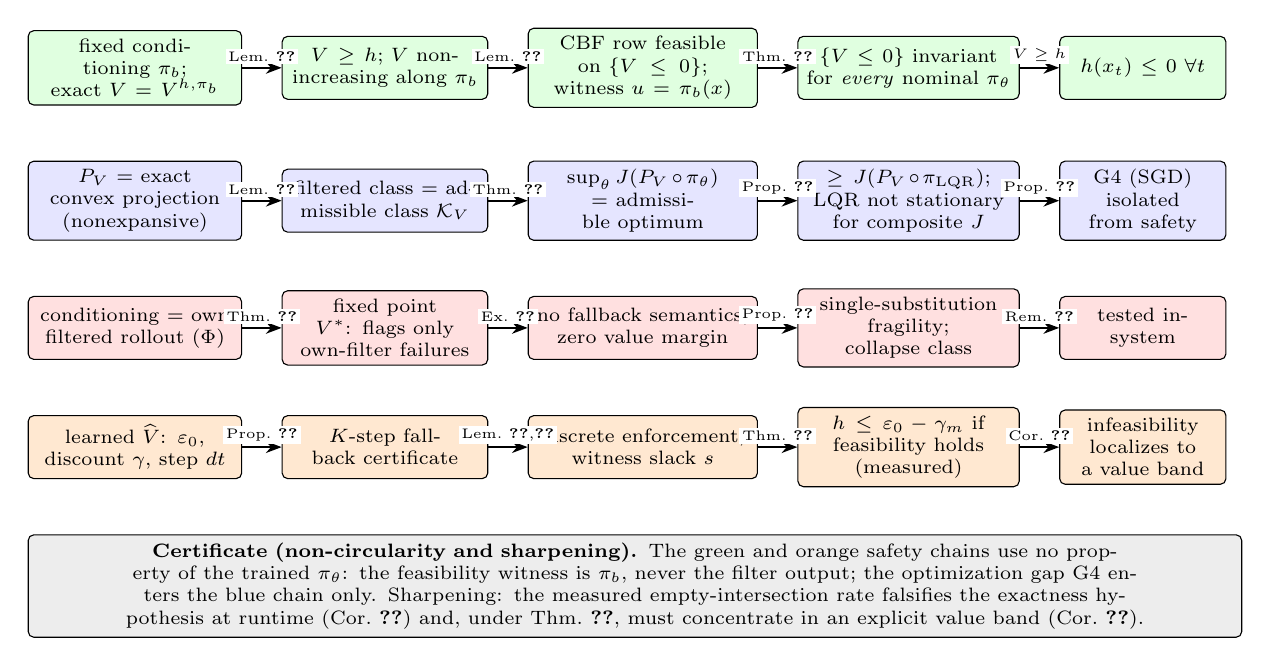
\begin{tikzpicture}[
  font=\scriptsize,
  box/.style={draw, rounded corners=2pt, align=center, inner sep=3pt, minimum height=8mm},
  gbox/.style={box, fill=green!12},
  obox/.style={box, fill=orange!18},
  rbox/.style={box, fill=red!12},
  bbox/.style={box, fill=blue!10},
  cbox/.style={box, fill=gray!14, text width=15.2cm},
  arr/.style={-{Stealth[length=2mm]}, semithick},
  lab/.style={font=\tiny, align=center, fill=white, inner sep=1pt}
]
\node[gbox, text width=2.5cm] (a1) {fixed conditioning $\pi_b$;\\ exact $V=\Vhp{\pi_b}$};
\node[gbox, right=5mm of a1, text width=2.4cm] (a2) {$V\ge h$;\ $V$ non-increasing along $\pi_b$};
\node[gbox, right=5mm of a2, text width=2.7cm] (a3) {CBF row feasible on $\{V\le 0\}$;\\ witness $u=\pi_b(x)$};
\node[gbox, right=5mm of a3, text width=2.6cm] (a4) {$\{V\le 0\}$ invariant for \emph{every} nominal $\pi_\theta$};
\node[gbox, right=5mm of a4, text width=1.9cm] (a5) {$h(x_t)\le 0$\ $\forall t$};
\draw[arr] (a1)--(a2) node[lab, midway, above=1pt] {Lem.~\ref{lem:mono}};
\draw[arr] (a2)--(a3) node[lab, midway, above=1pt] {Lem.~\ref{lem:feas}};
\draw[arr] (a3)--(a4) node[lab, midway, above=1pt] {Thm.~\ref{thm:inv}};
\draw[arr] (a4)--(a5) node[lab, midway, above=1pt] {$V\ge h$};
\node[bbox, below=7mm of a1, text width=2.5cm] (b1) {$P_V$ = exact convex projection\\ (nonexpansive)};
\node[bbox, right=5mm of b1, text width=2.4cm] (b2) {filtered class $=$ admissible class $\calK_V$};
\node[bbox, right=5mm of b2, text width=2.7cm] (b3) {$\sup_\theta J(P_V\!\circ\!\pi_\theta)$\\ $=$ admissible optimum};
\node[bbox, right=5mm of b3, text width=2.6cm] (b4) {$\ge J(P_V\!\circ\!\pi_{\mathrm{LQR}})$;\ LQR not stationary for composite $J$};
\node[bbox, right=5mm of b4, text width=1.9cm] (b5) {G4 (SGD) isolated from safety};
\draw[arr] (b1)--(b2) node[lab, midway, above=1pt] {Lem.~\ref{lem:range}};
\draw[arr] (b2)--(b3) node[lab, midway, above=1pt] {Thm.~\ref{thm:perf}};
\draw[arr] (b3)--(b4) node[lab, midway, above=1pt] {Prop.~\ref{prop:jac}};
\draw[arr] (b4)--(b5) node[lab, midway, above=1pt] {Prop.~\ref{prop:gaps}};
\node[rbox, below=7mm of b1, text width=2.5cm] (c1) {conditioning $=$ own filtered rollout ($\Phi$)};
\node[rbox, right=5mm of c1, text width=2.4cm] (c2) {fixed point $V^\ast$: flags only own-filter failures};
\node[rbox, right=5mm of c2, text width=2.7cm] (c3) {no fallback semantics;\\ zero value margin};
\node[rbox, right=5mm of c3, text width=2.6cm] (c4) {single-substitution fragility;\\ collapse class};
\node[rbox, right=5mm of c4, text width=1.9cm] (c5) {tested in-system};
\draw[arr] (c1)--(c2) node[lab, midway, above=1pt] {Thm.~\ref{thm:fixed}};
\draw[arr] (c2)--(c3) node[lab, midway, above=1pt] {Ex.~\ref{ex:nofallback}};
\draw[arr] (c3)--(c4) node[lab, midway, above=1pt] {Prop.~\ref{prop:frag}};
\draw[arr] (c4)--(c5) node[lab, midway, above=1pt] {Rem.~\ref{rem:toy}};
\node[obox, below=7mm of c1, text width=2.5cm] (d1) {learned $\Vhat$: $\varepsilon_0$, discount $\gamma$, step $dt$};
\node[obox, right=5mm of d1, text width=2.4cm] (d2) {$K$-step fallback certificate};
\node[obox, right=5mm of d2, text width=2.7cm] (d3) {discrete enforcement;\\ witness slack $s$};
\node[obox, right=5mm of d3, text width=2.6cm] (d4) {$h \le \varepsilon_0-\gamma_m$ if feasibility holds (measured)};
\node[obox, right=5mm of d4, text width=1.9cm] (d5) {infeasibility localizes to a value band};
\draw[arr] (d1)--(d2) node[lab, midway, above=1pt] {Prop.~\ref{prop:disc}};
\draw[arr] (d2)--(d3) node[lab, midway, above=1pt] {Lem.~\ref{lem:bridge},\ref{lem:witness}};
\draw[arr] (d3)--(d4) node[lab, midway, above=1pt] {Thm.~\ref{thm:margin}};
\draw[arr] (d4)--(d5) node[lab, midway, above=1pt] {Cor.~\ref{cor:band}};
\node[cbox, below=7mm of d1.south west, anchor=north west] (cert) {\textbf{Certificate (non-circularity and sharpening).} The green and orange safety chains use no property of the trained $\pi_\theta$: the feasibility witness is $\pi_b$, never the filter output; the optimization gap G4 enters the blue chain only. Sharpening: the measured empty-intersection rate falsifies the exactness hypothesis at runtime (Cor.~\ref{cor:falsify}) and, under Thm.~\ref{thm:margin}, must concentrate in an explicit value band (Cor.~\ref{cor:band}).};
\end{tikzpicture}
\caption{Logic chains of the safety, performance, degeneracy, and error-budget results}
\label{fig:chain}
\end{figure}

\section{Setup}\label{sec:di-setup}

\begin{definition}[Plant, flows, and policies]\label{def:plant}
\leavevmode
\begin{itemize}
\item $\calX\subset\R^n$ := the compact state space;
$\calU:=\prod_{i=1}^{m}[u_i^{\mathrm{lo}},u_i^{\mathrm{hi}}]\subset\R^m$ := the control box.
\item $f:\calX\to\R^n$, $g:\calX\to\R^{n\times m}$ := the drift and input vector fields of
$\dot x=f(x)+g(x)u$.
\item $F:\calX\times\calU\to\calX$ := the zero-order-hold flow map over one sampling period
$dt>0$. The discrete plant is $x_{k+1}=F(x_k,u_k)$.
\item A \textbf{\emph{policy}} is a map $\pi:\calX\to\calU$. $x_t^{\pi}$ := the continuous-time
closed-loop state; $x_k^{\pi,F}$ := the discrete closed-loop state.
\end{itemize}
\end{definition}

\begin{definition}[Safety cost and avoid set]\label{def:h}
$h:\calX\to[-a,b]\subseteq[-1,1]$ := the geometric safety cost, Lipschitz with constant $L_h$,
with $a,b>0$. $\calA:=\{x\in\calX: h(x)>0\}$ := the avoid set; $\calC:=\{h\le0\}$.
\end{definition}

\begin{definition}[Policy value function]\label{def:V}
For a policy $\pi$,
\[
\Vhp{\pi}(x) := \sup_{t\ge 0} h\big(x_t^{\pi}\big),
\qquad
\Vhp{\pi,F}(x) := \sup_{k\ge 0} h\big(x_k^{\pi,F}\big).
\]
\end{definition}

\begin{definition}[Discounted avoid operator]\label{def:T}
For $\gamma\in(0,1)$, a policy $\pi$, and $W$ in the space $\calB(\calX)$ of bounded functions,
\[
(\calT_\gamma^{\pi} W)(x) := \max\Big\{\,h(x),\ (1-\gamma)h(x) + \gamma\, W\big(F(x,\pi(x))\big)\Big\}.
\]
The clamped variant is $\bar\calT_\gamma^{\pi} := \mathrm{clip}_{[-1,1]}\circ\,\calT_\gamma^{\pi}$.
\end{definition}

\begin{definition}[CBF row, validity, and the HardNet box-aware filter]\label{def:filter}
Let $V\in C^1(\calX)$, $\alpha_s,\alpha_u>0$, and $\alpha_V(x):=\alpha_s$ if $V(x)\le0$,
$\alpha_u$ otherwise.
\begin{itemize}
\item $R_V(x):=\{u\in\calU: \grad V(x)^{\top}(f(x)+g(x)u)\le-\alpha_V(x)V(x)\}$ := the row set at
$x$, a closed convex subset of $\calU$.
\item $V$ is \textbf{\emph{valid}} on $\calS:=\{V\le0\}$ iff (i) $V\ge h$ on $\calX$ and
(ii) $R_V(x)\neq\emptyset$ for all $x\in\calS$.
\item $P_V:\calX\times\R^m\to\calU$ := the box-aware filter:
\[
P_V(x,u) :=
\begin{cases}
\displaystyle\arg\min_{w\in R_V(x)} \norm{w-u}^2, & R_V(x)\neq\emptyset,\\[4pt]
\displaystyle\arg\min_{w\in\calU}\ \big[\grad V(x)^{\top}(f(x)+g(x)w) + \alpha_V(x)V(x)\big], & R_V(x)=\emptyset,
\end{cases}
\]
the second branch flagged \textbf{\emph{infeasible}}.
\item The \textbf{\emph{filtered policy}} is $\pi^{V}:=P_V\circ\pi$.
\end{itemize}
\end{definition}

\begin{definition}[Task return]\label{def:J}
For an episode horizon $T_{\mathrm{ep}}\in\mathbb{N}$, discount $\gamma_T\in(0,1]$, an initial
distribution $\mu$ on $\calX$, and a stage cost $c:\calX\times\calU\to\R$ Lipschitz with
constants $L_c^x, L_c^u$,
\[
J(\kappa) := \E_{x_0\sim\mu}\Big[-\sum_{k=0}^{T_{\mathrm{ep}}-1}\gamma_T^{k}\, c\big(x_k,\kappa(x_k)\big)\Big],
\qquad x_{k+1}=F\big(x_k,\kappa(x_k)\big).
\]
\end{definition}

\begin{assumption}[Standing assumptions]\label{ass:standing}
\leavevmode
\begin{itemize}
\item[\textbf{(B1)}] $\calX$ is compact and forward invariant under $F$ for every admissible input sequence.
\item[\textbf{(B2)}] $f,g$ are Lipschitz and bounded on $\calX$;
$M:=\sup_{x\in\calX,u\in\calU}\norm{f(x)+g(x)u}<\infty$; $F$ is Lipschitz with constants
$L_F^x, L_F^u$.
\item[\textbf{(B3)}] $h$ is as in \cref{def:h}.
\item[\textbf{(B4)}] Every policy maps $\calX\to\calU$; every \emph{conditioning} policy $\pi_b$
is Lipschitz.
\item[\textbf{(B5)}] Statements invoking $\grad\Vhp{\pi}$ are read at points of differentiability
or in the viscosity sense \cite{so2024pncbf}; every deployed or learned $\Vhat$ is a Softplus
network, so all filter-side derivatives of $\Vhat$ are classical.
\end{itemize}
\end{assumption}

\begin{remark}[Instantiation]\label{rem:inst}
double integrator에서 (B1)은 velocity clamp $\norm{v}\le v_{\max}=2.5$와 arena 종료가 제공하고,
(B2)의 상수는 $M\le\sqrt{v_{\max}^2+2u_{\max}^2}\approx3.78$ ($u_{\max}=2$)이다. ZOH 하에서 DI의
flow는 $t$의 2차 다항식이므로 RK4 적분기가 $F$를 정확히 실현한다. 신경망이 대리하는 대상은 둘이다:
닫힌 형식이 없는 HJ variational inequality의 해 $\Vhp{\pi_b}$와 제약 최적 제어기. 대칭성,
매끄러움, 입력 제약은 전부 학습 이전에 고정된다.
\end{remark}

\section{Safety channel under exact conditioning}\label{sec:safety}

\textbf{직관.} certificate가 conditioning policy $\pi_b$의 정확한 policy value이면 안전은 nominal
policy가 무엇이든 성립한다. 사슬은 \cref{lem:mono}의 단조성 $\Rightarrow$ \cref{lem:feas}의
feasibility $\Rightarrow$ \cref{thm:inv}의 invariance이고, 두 따름정리가 이를 배포 계측과 잇는다.

\begin{lemma}[Monotonicity along the conditioning policy]\label{lem:mono}
Under \textup{(B3)--(B5)}, for every policy $\pi$ and every $x\in\calX$:
\begin{enumerate}[label=(\alph*)]
\item $t\mapsto \Vhp{\pi}(x_t^{\pi})$ is non-increasing on $[0,\infty)$;
\item $\Vhp{\pi}(x)\ge h(x)$;
\item at every differentiability point,
$\grad\Vhp{\pi}(x)^{\top}(f(x)+g(x)\pi(x))\le0$.
\end{enumerate}
The same holds for $\Vhp{\pi,F}$ with $k\in\mathbb{N}$ in place of $t$; (c) becomes
$\Vhp{\pi,F}(F(x,\pi(x)))\le\Vhp{\pi,F}(x)$.
\end{lemma}
\begin{proof}
Flow의 semigroup 성질로 $\Vhp{\pi}(x_t^{\pi})=\sup_{s\ge t}h(x_s^{\pi})$이고, $t$가 커질수록 sup의
대상 집합이 축소되므로 (a)가 성립한다. $s=t$ 항이 (b)를 준다. (a)에 의해 미분 가능한 점에서
$\tfrac{d}{dt}\Vhp{\pi}(x_t^\pi)|_{t=0}\le0$이며 이것이 (c)이다. 이산 경우도 동일하다.
\end{proof}

\begin{lemma}[Feasibility on the certified set, with witness]\label{lem:feas}
Let $V:=\Vhp{\pi_b}$ under \textup{(B3)--(B5)} and $\calS:=\{V\le0\}$. At every differentiability
point $x\in\calS$:
\begin{enumerate}[label=(\alph*)]
\item $\pi_b(x)\in R_V(x)$; in particular $R_V(x)\neq\emptyset$ and $V$ is valid on $\calS$;
\item if $\grad V(x)^{\top}g(x)=0$ (singular row), then $R_V(x)=\calU$.
\end{enumerate}
\end{lemma}
\begin{proof}
(a) \cref{lem:mono}(c)와 $V(x)\le0$에서
$\grad V(x)^{\top}(f(x)+g(x)\pi_b(x))\le0\le-\alpha_s V(x)$.
(b) 특이 행에서 row 조건은 $u$-독립인 $\grad V^{\top}f(x)\le-\alpha_s V(x)$로 축약되고, 이는 (a)의
좌변에서 $\grad V^\top g=0$을 대입한 것과 같으므로 모든 $u\in\calU$가 만족한다.
\end{proof}

\begin{theorem}[Nominal-independent invariance]\label{thm:inv}
Let $V:=\Vhp{\pi_b}$ satisfy the hypotheses of \cref{lem:feas}, and suppose the executed input
obeys $u(t)\in R_V(x(t))$ for all $t$, with the closed-loop solution existing in the
Carath\'eodory sense (\cref{rem:sol}). Then, for \emph{every} nominal policy $\pi_\theta$:
(a) $x(0)\in\calS\Rightarrow x(t)\in\calS$ for all $t\ge0$; (b) $h(x(t))\le0$ for all $t\ge0$.
\end{theorem}
\begin{proof}
Row 조건에서 $\calS$ 위의 매 시각 $\tfrac{d}{dt}V(x(t))\le-\alpha_s V(x(t))$이고, comparison
lemma로 $V(x(t))\le V(x(0))e^{-\alpha_s t}\le0$이므로 (a)이다. \cref{lem:mono}(b)의 $h\le V$가
(b)를 준다.
\end{proof}

\begin{remark}[Solution existence and boundary rigor]\label{rem:sol}
Filter 출력의 상태 의존 불연속에 따른 해의 존재와 Nagumo 경계 논증의 측도론적 세부는 CBF 문헌의
표준 처리 \cite{ames2017cbf,blanchini1999set}에 위임한다. 이 part의 다른 모든 배포 측
결과(\cref{sec:budget})는 이산 시간으로 정식화되어 이 조건을 필요로 하지 않는다.
\end{remark}

\begin{corollary}[Fallback semantics]\label{cor:fallback}
Under the hypotheses of \cref{lem:feas}, for every $x\in\calS$ running $\pi_b$ alone from $x$ is
safe for all time: $\sup_{t\ge0}h(x_t^{\pi_b})=V(x)\le0$, independently of the filter, of
$\pi_\theta$, and of how $V$ is deployed.
\end{corollary}
\begin{proof}
\cref{def:V}의 정의 자체이다.
\end{proof}

\begin{corollary}[Empty intersection falsifies exactness]\label{cor:falsify}
If there is $x\in\calX$ with $\Vhat(x)\le0$ and $R_{\Vhat}(x)=\emptyset$, then
$\Vhat\neq\Vhp{\pi}$ for every policy $\pi$. Consequently the measured empty-intersection rate on
$\{\Vhat\le0\}$ is, per step, the frequency of \emph{witnessed} violations of the exactness
hypothesis.
\end{corollary}
\begin{proof}
\cref{lem:feas}(a)의 대우이다.
\end{proof}

\begin{remark}[Singular events are not falsifications; the adopted instrumentation]\label{rem:cpsv2}
특이 플래그는 그 자체로 반증이 아니다(\cref{lem:feas}(b): exact value에서는 row가 자명하게
만족된다). 특이 행은 두 부류로 갈린다: \emph{row-satisfied} --- benign, 모든 $u$가 row를 만족하고
filter는 불활성 --- 와 \emph{row-violated} --- \cref{prop:flat}의 authority-loss 병리. exact
$V_{\calM}$은 인증 far field에서 clip floor에 포화해 전자를 대량 생산하므로(\cref{prop:vacuum}), 두
부류를 합산하는 계측은 정확성 자체를 벌점한다(raw infeasibility $0.87$--$0.91$). 채택된 계측
\texttt{infeasible\_v2} := empty-intersection 또는 (singular이면서 row-violated)는 정확히
\cref{cor:falsify}의 witnessed-violation 통계와 \cref{prop:flat}의 병리만을 계수한다. 실측: 모든
측정 시스템에서 empty-only 관례와 소수 4자리까지 일치하고, 재채점 lift는 learned $+0.03$--$0.05$ /
$V_{\calM}$ $+0.24$이다.
\end{remark}

\section{Control authority of the conditioning value}\label{sec:authority}

\textbf{직관.} Filter의 행동 능력은 row의 방향 $\grad V^{\top}g$에서 나오고, 그 방향은 conditioning
policy의 속도-감도에서 상속된다. 이 절은 그 상속을 정리로 만들고, 관측된 ceiling의 원인인
hazard-blind conditioning의 내부 평탄성을 특정한다.

\begin{proposition}[Gradient inheritance from the conditioning policy]\label{prop:grad}
Let $V:=\Vhp{\pi_b}$ and let $x$ be a point at which the maximizing time $t^{\ast}(x)$ is unique
and the flow $x\mapsto x^{\pi_b}_{t^{\ast}}$ is differentiable. Then by Danskin's theorem
\cite{danskin1966},
\[
\grad V(x) \;=\; \Big(\tfrac{\partial x^{\pi_b}_{t^{\ast}}}{\partial x}\Big)^{\!\top}\,\grad h\big(x^{\pi_b}_{t^{\ast}}\big),
\qquad
\norm{\grad V(x)^{\top} g(x)} \;\le\; L_h\, S_g,
\quad
S_g := \Big\lVert \tfrac{\partial x^{\pi_b}_{t^{\ast}}}{\partial x}\, g(x) \Big\rVert .
\]
For the double integrator with the deadband brake, at states whose maximizer is the stopped
point $p_{\mathrm{stop},i}=p_i+v_i\abs{v_i}/(2u_{\max})$,
\[
\frac{\partial V}{\partial v_i} \;=\; \frac{\abs{v_i}}{u_{\max}}\,\partial_i h\big(p_{\mathrm{stop}}\big):
\]
the braking-distance geometry is embedded in the gradient, nonvanishing whenever $v_i\neq0$ and
growing linearly in speed.
\end{proposition}
\begin{proof}
$V(x)=\max_{t}h(x_t^{\pi_b}(x))$는 compact 시간 구간 위 매개변수 최대이고, 유일 최대점에서
Danskin으로 미분이 통과한다. 둘째 부등식은 chain rule과 $\norm{\grad h}\le L_h$이다. Brake의 경우
$\partial p_{\mathrm{stop},i}/\partial v_i=\abs{v_i}/u_{\max}$이므로 성분별 chain rule로 주장이
따른다.
\end{proof}

\begin{proposition}[Interior flatness of hazard-blind conditioning]\label{prop:flat}
Suppose an open set $O\subseteq\calX$ on which the $\pi_b$-trajectory from every $x'\in O$
attains the clip ceiling, $\sup_t h=b$. Then on $O$: $V\equiv b$, $\grad V\equiv0$, every row is
singular, and the row with $\alpha_u V>0$ is infeasible with a direction-free least-violating
objective --- the filter retains no first-order authority precisely where recovery is demanded.
\end{proposition}
\begin{proof}
열린 집합 위 상수이므로 $\grad V=0$. Row 좌변은 $0$, 우변은 $-\alpha_u b<0$이므로 모든 $u$가
위반하고, least-violating 목적이 $u$-독립이라 방향이 없다.
\end{proof}

\begin{remark}[Measured correlates]\label{rem:authmeas}
unfiltered $\pi_b$ 재-roll 종점은 speed $\approx2.07$ ($\approx v_{\max}$), $13\%$
post-collision의 hazard-blind charger 특성이고, 관측된 singular 성분 $0.089$--$0.166$과
filter-active stuck $0.90$--$0.95$가 \cref{prop:flat}의 코드-측 상관물이다.
\end{remark}

\begin{remark}[Noise as a mollifier: the second role of $\sigma$]\label{rem:mollify}
stored-rollout conditioning의 label은 per-rollout 확률변수이고, 평균제곱 회귀의 극한은
\[
m(x) \;:=\; \E_{\xi}\Big[\,\sup_{t}\,h\big(x_t^{\,\pi_\theta+\xi,\,P}\big)\Big],
\]
즉 basin indicator의 $\sigma$-mollification이다. $m$은 gradient를 폭 $\sim\sigma\sqrt{T}$ 급의
band에 분산시켜 filter에 authority를 공급한다: \cref{prop:noise}의 margin 역할에 더한 $\sigma$의 제2
기능이다. 노이즈를 제거한 lagged conditioning은 margin과 authority를 동시에 제거했다.
\end{remark}

\begin{proposition}[Benign interior flatness of the exact certificate]\label{prop:vacuum}
Suppose an open set $O\subseteq\{V\le0\}$ on which the deployed (clipped) certificate saturates
at the floor, $V\equiv-1$. Then on $O$:
\begin{enumerate}[label=(\alph*)]
\item $\grad V\equiv0$ and every row is singular;
\item with margin $\gamma_m<1$ the row is $u$-independently \emph{satisfied}, so $R_V(x)=\calU$
and the filter is inactive;
\item every policy-objective term that reads the certificate --- the region gates, the terminal
$V(x_T)$, and the filter path of the BPTT graph --- contributes identically zero $\theta$-gradient
from rollout segments confined to $O$; the only credit reaching $\pi_\theta$ from such segments
is the $T$-step task return.
\end{enumerate}
\end{proposition}
\begin{proof}
(a) 열린 집합 위 상수이다. (b) $\grad V^{\top}f=0$과 $V+\gamma_m=\gamma_m-1<0$을 row에 대입하면
모든 $u$가 만족한다. (c) 각 항이 $V$와 $\grad V$를 통해서만 $\theta$에 닿으므로, 상수 $V$와 영
gradient에서 기여가 소멸한다.
\end{proof}

\begin{remark}[Measured credit-horizon gap]\label{rem:credit}
\cref{prop:flat}의 병리적 평탄(위반)과 대조되는 benign 평탄(만족)이며, 병리 대신 \emph{유도 공백}을
남긴다. 실측이 (c)의 결과를 계량한다: open-area stall onset에서 filtered-LQR 탈출의 도달 소요는
$4.65$--$7.85$\,s(평균 $6.11$; 15건 중 10건 탈출)로 BPTT 창 $T\,dt=1.5$\,s의 $3$--$5\times$이고
초과율 $100\%$다. 재선택 peak 이후 cps $-0.0589$는 reach $-0.0295$와 stuck $+0.0285$로 갈리고
collision은 평탄하다 --- 안전 채널 절연과 정합한다. horizon 연장은 무효다: $T=60$($3.0$\,s)은 최단
payback에도 미달하고, 커버에는 $T\approx93$--$157$이 필요하나 메모리·처리량·stall 평형에서의 탐색
부재로 비현실적이다. 학습 $\Vhat$의 내부 gradient가 사실상 항행 유도를 겸했다는 것이 학습
certificate 성능의 숨은 기제였고 정확성이 그것을 제거했다 --- 남은 격차는 이 공백의 성능-채널
문제다.
\end{remark}

\section{Performance channel}\label{sec:perf}

\textbf{직관 (표현력 무손실).} Filter가 성능을 해치는 경로는 둘이다: 도달 가능한 controller class를
좁히거나, 최적화 landscape를 왜곡하거나. 이 절은 전자가 발생하지 않음을 보인다 --- 배포되는
box-aware filter가 볼록 집합 위의 정확한 유클리드 사영이라는 사실 하나에서 filtered class가
admissible class와 일치하고(\cref{lem:range}) 사영이 nonexpansive여서 universal approximation이
filter를 그대로 통과한다(\cref{thm:perf}). 후자에 대해서는 \cref{prop:jac}이 LQR이 composite
목적함수의 stationary point가 아님을 보인다.

\begin{definition}[Admissible controller classes]\label{def:adm}
Given $V\in C^1(\calX)$ with $R_V(x)\neq\emptyset$ for all $x\in\calX$:
\[
\calK_V := \{\kappa:\calX\to\calU\ \text{measurable}:\ \kappa(x)\in R_V(x)\ \forall x\},
\qquad
\calK_V^{L} := \{\kappa\in\calK_V:\ \kappa\ \text{Lipschitz}\}.
\]
\end{definition}

\begin{lemma}[Filter range identity]\label{lem:range}
Under the hypothesis of \cref{def:adm}: (a) $P_V\circ\kappa=\kappa$ for every $\kappa\in\calK_V$;
(b) $P_V\circ\pi\in\calK_V$ for every measurable $\pi:\calX\to\R^m$. Hence
$\{P_V\circ\pi:\pi\ \text{measurable}\}=\calK_V$.
\end{lemma}
\begin{proof}
(a) 닫힌 볼록 집합의 원소는 자기 자신으로 사영된다. (b) \cref{def:filter}에서
$R_V(x)\neq\emptyset$이면 출력이 $R_V(x)$의 원소이다.
\end{proof}

\begin{lemma}[Nonexpansiveness]\label{lem:nonexp}
For every $x$ with $R_V(x)\neq\emptyset$ and all $u_1,u_2\in\R^m$:
$\norm{P_V(x,u_1)-P_V(x,u_2)}\le\norm{u_1-u_2}$.
\end{lemma}
\begin{proof}
닫힌 볼록 집합 위의 유클리드 사영 $P$는 $\inner{u_i-P(u_i)}{w-P(u_i)}\le0$을 모든
$w\in R_V(x)$에 대해 만족한다. $w$에 서로의 사영점을 대입해 더하면
\[
\norm{P(u_1)-P(u_2)}^2 \;\le\; \inner{u_1-u_2}{P(u_1)-P(u_2)} \;\le\; \norm{u_1-u_2}\,\norm{P(u_1)-P(u_2)}. \qedhere
\]
\end{proof}

\begin{lemma}[Return continuity against a Lipschitz feedback]\label{lem:Jcont}
Under \textup{(B1)--(B2)} and \cref{def:J}, let $\kappa_1$ be $L_\kappa$-Lipschitz, $\kappa_2$
measurable, and $\varepsilon:=\sup_{x\in\calX}\norm{\kappa_1(x)-\kappa_2(x)}$. Then
\[
\abs{J(\kappa_1)-J(\kappa_2)} \;\le\; L_J\,\varepsilon,
\qquad
L_J := \sum_{k=0}^{T_{\mathrm{ep}}-1}\gamma_T^{k}\Big[(L_c^x+L_c^uL_\kappa)\,L_F^u\,\tfrac{\rho^{k}-1}{\rho-1} + L_c^u\Big],
\quad \rho := L_F^x+L_F^uL_\kappa
\]
(with $\tfrac{\rho^k-1}{\rho-1}$ read as $k$ when $\rho=1$).
\end{lemma}
\begin{proof}
동일 초기조건의 두 closed loop 편차 $d_k:=\norm{x_k^{(1)}-x_k^{(2)}}$에 대해
$d_{k+1}\le\rho\,d_k+L_F^u\varepsilon$이므로
$d_k\le L_F^u\varepsilon(\rho^{k}-1)/(\rho-1)$이다. 단계 비용 편차는
$(L_c^x+L_c^uL_\kappa)d_k+L_c^u\varepsilon$ 이하이고, 이를 $\gamma_T^k$ 가중 합산하면 주장이
나온다.
\end{proof}

\begin{theorem}[No representational loss]\label{thm:perf}
Let $\Vhat\in C^1(\calX)$ with $R_{\Vhat}(x)\neq\emptyset$ for all $x\in\calX$, and let the
nominal class be dense in $(C(\calX,\R^m),\norm{\cdot}_\infty)$. Then:
\begin{enumerate}[label=(\alph*)]
\item $\displaystyle \sup_{\kappa\in\calK_{\Vhat}^{L}} J(\kappa)\ \le\ \sup_{\theta} J\big(P_{\Vhat}\circ\pi_\theta\big)\ \le\ \sup_{\kappa\in\calK_{\Vhat}} J(\kappa)$;
\item if in addition $x\mapsto P_{\Vhat}(x,\pi_{\mathrm{LQR}}(x))$ is Lipschitz (hypothesis
\textup{(R)}), then $\sup_\theta J(P_{\Vhat}\circ\pi_\theta)\ge J(P_{\Vhat}\circ\pi_{\mathrm{LQR}})$;
and for every Lipschitz $\pi_b\in\calK_{\Vhat}$,
$\sup_\theta J(P_{\Vhat}\circ\pi_\theta)\ge J(\pi_b)$.
\end{enumerate}
\end{theorem}
\begin{proof}
(a) 하한: $\kappa\in\calK^L_{\Vhat}$, $\delta>0$을 고정하고 조밀성으로
$\sup_x\norm{\pi_\theta(x)-\kappa(x)}\le\varepsilon$인 $\theta$를 고른다. \cref{lem:range}(a)와
\cref{lem:nonexp}에서 $\norm{P_{\Vhat}(x,\pi_\theta(x))-\kappa(x)}\le\varepsilon$이고,
\cref{lem:Jcont}로 $\abs{J(P_{\Vhat}\circ\pi_\theta)-J(\kappa)}\le L_J\varepsilon\le\delta$가
되도록 $\varepsilon$을 잡는다. 상한: \cref{lem:range}(b). (b) clamp$\circ$linear는 Lipschitz이므로
$\pi_\theta\to\pi_{\mathrm{LQR}}$ 균등 근사를 잡고 \cref{lem:nonexp}, (R), \cref{lem:Jcont}를
적용한다. $\pi_b$의 경우 \cref{lem:range}(a)에서 $J(\pi_b)=J(P\circ\pi_b)$이다.
\end{proof}

\begin{remark}[Scope and relation to HardNet]\label{rem:hardnet}
(a)의 Lipschitz-대-measurable sup 간극은 기술적 잔여(O7)이다. HardNet의 universal approximation
정리 \cite{min2024hardnet}는 base half-space projection class에 대한 대응 결과이고, 여기서는 배포
filter가 half-space$\cap$box 위의 \emph{정확한} 볼록 사영이라는 사실이 \cref{lem:nonexp}를 통해 더
짧은 경로를 준다. 결론: JT의 최적화 대상은 해당 certificate 아래에서 도달 가능한 최고 성능 그
자체이며, filtered-LQR은 그 하한이다.
\end{remark}

\begin{proposition}[Composite first-order structure; the optimal nominal is not LQR]\label{prop:jac}
Consider the base half-space projection with regularizer $\varepsilon_h\ge0$,
\[
u_{\mathrm{safe}} \;=\; u - \frac{A(x)}{\norm{A(x)}^2+\varepsilon_h^2}\,\big(A(x)^{\top}u - b(x)\big)_+ ,
\qquad A(x) := g(x)^{\top}\grad V(x),\ \ b(x) := -\grad V^{\top}f - \alpha_V V .
\]
At every $(x,u)$ with $A^{\top}u>b$ at which no box clamp binds,
\[
\frac{\partial u_{\mathrm{safe}}}{\partial u} \;=\; I - \frac{A A^{\top}}{\norm{A}^2+\varepsilon_h^2} \;=:\; \Pi(x).
\]
Consequently, almost everywhere along closed-loop trajectories, the chain-rule factor of
$\grad_\theta J(P\circ\pi_\theta)$ at active steps is $\Pi(x_t)$, which annihilates the
row-normal direction. Hence first-order stationarity of $\pi_{\mathrm{LQR}}$ for the
unconstrained LQ objective does not imply stationarity for $\theta\mapsto J(P\circ\pi_\theta)$;
the two coincide only if the active set has closed-loop visitation measure zero, or the
row-normal component of the return gradient vanishes on it. Scope: base-projection regime;
activation boundaries, box facets, and candidate-selection ties are excluded as measure-zero
kink sets.
\end{proposition}
\begin{proof}
활성 영역에서 $(A^{\top}u-b)_+=A^{\top}u-b$는 $u$에 대해 선형이므로 미분하면 주어진 $\Pi(x)$가
나온다. 나머지는 chain rule의 직접 결과이다.
\end{proof}

\textbf{해석 --- scope 정정.} $\Pi$의 null space는 사실이지만, ``학습이 filter 개입 크기를 낮추는
방향으로 nominal을 이동시킨다''는 이전 판의 해석은 기각한다: friction 항
$\lambda_f\norm{u_{\mathrm{safe}}-u_{\mathrm{nom}}}^2$을 부과해도 active-band 개입 크기가
$1.335\approx1.341$로 불변이었다 --- 경계 개입의 대부분은 과제 기하가 강제하는 \emph{필요
성분}이지 무상 법선 표류가 아니다. friction의 실효과는 per-step 개입 축소가 아니라 open-area
행동 수준의 stuck 감소였다(감소분의 $80\%$; cps\_v2 $+0.007$).

\begin{remark}[Equivalence standard for branch-discrete filters]\label{rem:equiv}
\cref{prop:jac}의 scope가 배제한 measure-zero kink 집합은 구현 등가성의 정의를 바꾼다: 선택자가
branch-discrete이므로 부동소수점 연산 순서가 다른 두 구현은 궤적 bit-parity를 원리적으로 달성할 수
없다 --- reference 구현 자신이 $10^{-7}$ state jitter에 $24/512$ 행동과 $114/256$ 궤적을 뒤집는다.
올바른 등가성은 \emph{함수 parity}($\abs V$ 차 $\le10^{-6}$, $\abs{\grad V}$ 차 $\le10^{-5}$)와
\emph{안전 등가성}(paired-episode collision·region-flag delta 허용치)의 결합이고, verdict-급
비교는 같은 구현끼리로 정합화한다. parity 시험은 라이브러리 버전 변경마다 재실행된다.
\end{remark}

\begin{proposition}[Dual role of the task cost under self-conditioning]\label{prop:taskcost}
\leavevmode
\begin{enumerate}[label=(\alph*)]
\item Under a $\pi_\theta$-independent conditioning, \cref{thm:perf} holds for \emph{every} task
return $J$ of the form \cref{def:J}: the cost choice is safety-free, and a filter-friction term
may be added to $J$ without affecting any certificate claim.
\item Under self-conditioning, $J$ acquires a second role --- label-distribution generator. For
the DI cost with vanishing velocity and effort weights the unconstrained optimum approaches the
time-optimal saturating controller, a hazard-blind charger, which by \cref{prop:flat} degrades
the certificate's authority; conversely a friction term starves the label's unsafe signal. The
cost that is optimal for role one is adversarial for role two.
\end{enumerate}
Scope: (a) is structural and was exercised in-system --- the friction term was added under the
$\pi_\theta$-independent $V_{\calM}$ and every certificate statistic stayed flat; (b) is
sketch-grade, its charger limit anchored by the measured re-roll speed $\approx2.07\approx
v_{\max}$.
\end{proposition}
\begin{proof}
(a)는 \cref{thm:perf}의 증명이 $J$의 형태만 사용한다는 사실과 friction 항이 같은 형태라는
사실이다. (b): label 분포가 $\pi_\theta$의 함수이므로 $J$-최적화가 label을 성형한다; charger
극한과 그 authority 결과는 \cref{prop:flat}, unsafe-signal 기아는 \cref{sec:degen}의 기제이다.
\end{proof}

\section{Exact policy iteration}\label{sec:pi}

\begin{definition}[Certified sets]\label{def:sets}
$\calS_\pi:=\{\Vhp{\pi}\le0\}$ for a policy $\pi$ with well-posed closed loop;
$\calS^{\cup}:=\bigcup_{\pi}\calS_\pi$ over all such policies.
\end{definition}

\begin{theorem}[Monotone joint improvement under exact evaluation]\label{thm:pi}
Let $\pi_{b,0}$ satisfy \textup{(B4)}, let $V_k:=\Vhp{\pi_{b,k}}$ be evaluated exactly, and let
$\pi_{b,k+1}:=P_{V_k}\circ\pi_\theta^{(k)}$ for an arbitrary nominal sequence, with the
enforcement hypotheses of \cref{thm:inv} at each stage. Then for all $k$:
(a) $\calS_k:=\calS_{\pi_{b,k}}$ satisfies $\calS_k\subseteq\calS_{k+1}\subseteq\calS^{\cup}$;
(b) every deployment stage is collision-free from $\calS_k$;
(c) the confined-behavior optimum $J^{\star}(\calS)$ is non-decreasing along $k$.
\end{theorem}
\begin{proof}
(a) $x\in\calS_k$를 고정한다. \cref{thm:inv}로 $\pi_{b,k+1}$-궤적이 $\calS_k$에 머물고 그 위에서
$h\le V_k\le0$이므로 $V_{k+1}(x)\le0$이다. (b)는 \cref{thm:inv}(b)이다. (c)는
$\calS\mapsto J^{\star}(\calS)$가 집합 포함에 단조라는 사실과 (a)의 결합이다.
\end{proof}

\textbf{해석.} \cref{thm:pi}가 ``safety와 performance의 동시 향상''의 이상화된 증명이다: 매 단계
안전은 exact하고, 인증 집합은 단조 성장하며, 그 집합에 갇힌 이상 최적 성능도 단조 증가한다. 상충의
자유변수는 안전이 아니라 certificate의 크기뿐이다. 따라서 실제 시스템의 붕괴는 어느 가정이 깨져
발생하는가 --- 답은 $V_k$의 \emph{평가}이며, 다음 절이 그 대상을 특정한다.

\section{Degeneracy of self-referential evaluation}\label{sec:degen}

\textbf{직관.} 구현은 value label을 자기 rollout의 $h$-sequence에서 만든다. 즉 학습이 겨냥하는
population 대상은 고정 $\pi_b$의 값이 아니라 자기참조 operator $\Phi$의 고정점이다. 이 절은 (i)
고정 conditioning은 $\gamma$-contraction이어서 학습이 잘 정의되는 반면, (ii) $\Phi$의 고정점은
``자기 filter의 잔여 위험''만을 기록하는 margin-free 퇴화 certificate임을, (iii) baseline이 그럼에도
살아 있는 이유는 탐사 노이즈가 임차해 주는 암묵적 margin임을 보인다.

\begin{definition}[Self-referential evaluation operator]\label{def:phi}
Given a nominal $\pi_\theta$ and the filter of \cref{def:filter} (whose least-violating fallback
makes $\kappa_V:=P_V\circ\pi_\theta$ defined for every $V\in C(\calX)$),
\[
\Phi(V)(x) \;:=\; \sup_{k\ge 0}\, h\big(x_k^{\kappa_V,F}\big).
\]
\end{definition}

\begin{proposition}[Fixed conditioning is a $\gamma$-contraction]\label{prop:contr}
For every policy $\pi$, every $\gamma\in(0,1)$ and all $W_1,W_2\in\calB(\calX)$:
$\norm{\calT_\gamma^{\pi}W_1-\calT_\gamma^{\pi}W_2}_\infty\le\gamma\norm{W_1-W_2}_\infty$, and
the same for $\bar\calT_\gamma^{\pi}$. Hence each admits a unique fixed point $\tV_\gamma^{\pi}$.
Moreover, for every $x$ whose $\pi$-trajectory attains its supremum at a finite index,
$\tV_\gamma^{\pi}(x)\to\Vhp{\pi,F}(x)$ as $\gamma\uparrow1$.
\end{proposition}
\begin{proof}
$\abs{\max(a,b_1)-\max(a,b_2)}\le\abs{b_1-b_2}$에서 contraction이 따르고, clip은 1-Lipschitz이므로
상수가 보존된다. 극한 주장은 \cref{prop:disc}(a),(b)에서 따른다. 이 형태의 discounted safety
Bellman contraction은 \cite{fisac2019bridging}의 계보이다.
\end{proof}

\begin{theorem}[Fixed points of the self-referential evaluation are degenerate]\label{thm:fixed}
Let $V^\ast\in C(\calX)$ satisfy $V^\ast=\Phi(V^\ast)$, write
$\kappa^\ast:=P_{V^\ast}\circ\pi_\theta$ and $\calS^\ast:=\{V^\ast\le0\}$. Then:
\begin{enumerate}[label=(\alph*)]
\item $V^\ast\ge h$ on $\calX$;
\item $\{V^\ast>0\}=\calD(V^\ast):=\{x:\exists k,\ x_k^{\kappa^\ast,F}\in\calA\}$: the certificate
flags exactly the failure set of \emph{its own} filtered closed loop, and constrains
$\Vhp{\pi_\theta}$ in no way;
\item if $\emptyset\neq\calS^\ast\neq\calX$ and $\calX$ is connected, then
$\sup_{x\in\calS^\ast}V^\ast(x)=0$: for every $\eta>0$ there exist certified states whose
own-filter trajectory approaches contact within $\eta$.
\end{enumerate}
\end{theorem}
\begin{proof}
(a) $k=0$ 항. (b) 고정점 정의에서
$V^\ast(x)>0\iff\sup_k h(x_k^{\kappa^\ast,F})>0\iff x\in\calD(V^\ast)$.
(c) $\calS^\ast$는 닫힌 진부분집합이고 $\calX$가 연결이므로 경계점 $x^\dagger$에서 연속성으로
$V^\ast(x^\dagger)=0$이고, (b)에 의해 그 값은 그 상태에서 출발한 $\kappa^\ast$-궤적의 최근접
$h$-값이다.
\end{proof}

\begin{example}[No fallback: a three-state instance]\label{ex:nofallback}
States $\{0,1,2\}$ with $h(0)=b>0$, $h(1)=h(2)=-a$; $0,2$ absorbing; $\calU=\{\ell,r\}$ with
$F(1,\ell)=0$, $F(1,r)=2$; $\pi_\theta(1)=\ell$. For any $V$ with $V(0)>0\ge V(1),V(2)$ the
filter overrides at state $1$ to $r$, so $\Phi(V)(1)=-a$. Hence
$V^\ast(0)=b$, $V^\ast(1)=V^\ast(2)=-a$ is a fixed point with $V^\ast(1)\le0$ while
$\Vhp{\pi_\theta}(1)=b$: the certificate asserts nothing about any $V^\ast$-independent policy.
\cref{cor:fallback}과의 대조가 건전한 conditioning과의 형식적 분리선이다.
\end{example}

\begin{proposition}[Single-substitution fragility]\label{prop:frag}
Suppose hypothesis \textup{(H)}: there exist $x_0\in\calS^\ast$, an index $j$, and $u'\in\calU$
such that the $\kappa^\ast$-trajectory from $x_0$ satisfies
$F(x_j,u')\in\calD(V^\ast)\cup\calA$. Then the trajectory that executes $\kappa^\ast$ at every
step except $u'$ at step $j$ enters $\calA$.
\end{proposition}
\begin{proof}
$F(x_j,u')\in\calA$이면 즉시 위반이다. $F(x_j,u')\in\calD(V^\ast)$이면 \cref{thm:fixed}(b)에 의해
그 상태에서의 후속 궤적이 $\calA$에 진입한다.
\end{proof}

\begin{remark}[Numerical instantiation and the collapse signature]\label{rem:toy}
\textup{(H)}와 \cref{thm:fixed}의 기제는 210-상태 관성 testbed에서 수치로 실증되었다: unfiltered
nominal의 위반율 $100\%$인 문제에서, 고정 raw conditioning의 certificate는 161/210 셀을 위험으로
표시하고 $15\%$ action-noise 평가에서 위반 $0.000$을 유지한 반면, 자기참조 conditioning의 고정점은
25/210 셀만 표시하고 동일 노이즈에서 위반 $0.93$을 보였다. 이는 유한 사례의 기제 실증이며 학습된
시스템의 정확한 고정점에 대한 주장이 아니다. 학습 시스템에서 같은 퇴화의 함수근사 실현이 관측된
collapse 서명이다: $\Vhat\to$ 평탄, $\grad\Vhat^{\top}g\to0$, filter 불활성, 그 후 파국.
\end{remark}

\begin{proposition}[Worst-case-noise conditioning purchases margin]\label{prop:noise}
For $\bar\sigma\ge0$ define
\[
\Phi_{\bar\sigma}(V)(x) := \sup_{\{\xi_k\}:\norm{\xi_k}\le\bar\sigma}\ \sup_{k\ge0}\ h(x_k),
\qquad x_{k+1}=F\big(x_k,\ \mathrm{sat}_{\calU}(\kappa_V(x_k)+\xi_k)\big).
\]
At any fixed point $V^\ast_{\bar\sigma}$, every certified state
$x\in\{V^\ast_{\bar\sigma}\le0\}$ satisfies $\sup_k h(x_k)\le0$ along \emph{every}
$\bar\sigma$-bounded perturbation sequence of the filtered execution.
\end{proposition}
\begin{proof}
고정점에서 $V^\ast_{\bar\sigma}(x)$가 정의상 그 worst-case 값이다.
\end{proof}

\begin{remark}[The baseline's implicit margin]\label{rem:sigma}
가우시안 $\sigma$-노이즈 수집 $+$ 평균제곱 회귀 $+$ unsafe-fraction 목표의 adaptive $\sigma$로 된
구현은 $\Phi$와 $\Phi_{\bar\sigma}$ 사이에 놓인다: label의 노이즈가 \cref{prop:noise}의 margin을
확률적으로 임차하고, 목표 unsafe fraction과 $\sigma_{\min}$이 그 암묵적 margin knob이다. 이것이
baseline이 생존하는 이유이자 노이즈가 부족해진 policy-iteration 시도들이 동일하게 붕괴한 이유다.
\end{remark}

\begin{proposition}[Sound lagged-policy conditioning]\label{prop:lagged}
Let $\pi_{b}$ be a $V$-independent, unfiltered policy copy updated by
$\theta_b\leftarrow(1-\tau_b)\theta_b+\tau_b\theta_\pi$ with $\tau_b$ small relative to the
effective value-learning rate. Then:
\begin{enumerate}[label=(\alph*)]
\item between policy updates the value target is the fixed point of $\bar\calT_\gamma^{\pi_b}$,
whose exact limit is the valid certificate of \cref{lem:feas,thm:inv};
\item with zero tail weight the label of a stored pair is a deterministic function of that pair
given $\pi_b$, so a single visit yields a permanently correct label; for positive tail weight the
label depends on the target network through the bootstrap tail evaluated at the re-roll
endpoint --- the mixed operator of \cref{sec:mixed}, whose endpoint lies off the collection
support;
\item tracking of the slowly varying family follows the standard two-timescale
stochastic-approximation argument \cite{borkar1997two} (sketch).
\end{enumerate}
\end{proposition}
\begin{proof}
(a)는 \cref{prop:contr}와 \cref{lem:feas}의 결합, (b)의 첫 절반은 conditioning rollout의
결정론에서 즉시 따르고 둘째 절반은 \cref{def:mixedop}의 정의이다. (c)는 스케치 등급으로 남긴다.
\end{proof}

\section{The implemented label operator: the mixed estimator}\label{sec:mixed}

\textbf{직관.} 구현된 label은 \cref{def:T}의 $\calT_\gamma^{\pi_b}$가 아니라 truncated rollout과
bootstrap tail의 rectified 혼합이다. 이 절은 그 연산자를 정의하고 수렴상수·두 편향 채널·고장
방향을 정리로 만든다.

\begin{definition}[Mixed estimator]\label{def:mixedop}
For a horizon $T$, mixing weight $c\in[0,1]$, and discount $\gamma$, define for
$W\in\calB(\calX)$:
\begin{itemize}
\item $\mathrm{lhs}_T(x)$ := the $T$-step discounted-avoid value of the $h$-sequence along
$\pi_b$ from $x$ ($W$-independent);
\item $\mathrm{rhs}_T(W)(x)$ := the within-horizon integral term $+\ \gamma^{T}W(x_T^{\pi_b})$;
\item $M_c(W)(x) := \mathrm{lhs}_T(x) + c\,(\mathrm{rhs}_T(W)(x)-\mathrm{lhs}_T(x))_{+}$.
\end{itemize}
\end{definition}

\begin{theorem}[Contraction, bias channels, and failure direction]\label{thm:mixed}
Let $\tV:=\tV_\gamma^{\pi_b}$ and $\beta:=c\,\gamma^{T}$. Then:
\begin{enumerate}[label=(\alph*)]
\item $M_c$ is a sup-norm contraction with modulus $\beta$, with a unique fixed point
$V_\infty^{c}$;
\item (truncation channel, one-sided) $M_c(\tV)-\tV=-(1-c)\,g_{\mathrm{trunc}}\le0$ with
$g_{\mathrm{trunc}}:=(\mathrm{rhs}_T(\tV)-\mathrm{lhs}_T)_{+}$, hence
$\norm{V_\infty^{c}-\tV}_\infty\le(1-c)\norm{g_{\mathrm{trunc}}}_\infty/(1-\beta)$, and the bias
is downward: hazards realized only beyond the horizon are under-weighted;
\item (tail channel, rectified) if the tail is evaluated with error $e$ at $x_T$, the
per-application label perturbation is $c[(A+\gamma^{T}e)_{+}-(A)_{+}]$ with
$A:=\mathrm{rhs}_T(\tV)-\mathrm{lhs}_T$, bounded by $\beta\abs{e}$ and, for zero-mean $e$,
non-negative in expectation: the tail channel biases upward only. Hence the estimation failure
mode is structurally conservative, and
\[
\big|M_c^{e}(W) - M_1(\tV)\big| \;\le\; (1-c)\,g_{\mathrm{trunc}} + \beta\big(\norm{W-\tV}_\infty + \abs{e}\big).
\]
\end{enumerate}
Scope: (a)--(c) complete at the stated level; the fixed-point version of (c) under an
off-support error model is sketch-grade.
\end{theorem}
\begin{proof}
(a) $(\cdot)_+$는 1-Lipschitz이고 $W$-의존은 $\gamma^{T}W(x_T)$뿐이므로
$\abs{M_c(W_1)-M_c(W_2)}\le\beta\norm{W_1-W_2}_\infty$. (b) $c=1$에서
$M_1(W)=\max\{\mathrm{lhs}_T,\mathrm{rhs}_T(W)\}$는 정확한 $T$-step backup이고 $\tV$는 그
고정점이므로 $M_c(\tV)-\tV=(c-1)g_{\mathrm{trunc}}\le0$이며, 고정점 섭동
$\norm{V_\infty^{c}-\tV}\le\norm{M_c(\tV)-\tV}/(1-\beta)$로 닫힌다. (c) 첫 부등식은 $(\cdot)_+$의
1-Lipschitz, 기대값 부등식은 Jensen
$\E(A+\gamma^{T}e)_{+}\ge(A+\gamma^{T}\E e)_{+}=(A)_{+}$이며, 마지막 상계는 (b)의 잔차와 (a)의
Lipschitz를 삼각부등식으로 결합한 것이다.
\end{proof}

\begin{remark}[Measured instantiation]\label{rem:instmix}
두 실험(비제한 schedule 대 단일 축 $c_{\mathrm{final}}$ $0.9\to0.5$)의 측정이 \cref{thm:mixed}의 각
항에 대응한다.
\begin{center}\small
\begin{tabular}{lcc}
\toprule
quantity & Exp 1 ($c_{\mathrm{final}}{=}0.9$) & Exp 2 (cap $c_{\mathrm{final}}{=}0.5$)\\
\midrule
$\beta$ endpoint / amplification $\tfrac{1}{1-\beta}$ & $0.84$ / $6.1\times$ & $\le0.47$ / $\le1.9\times$\\
tail push probe, early$\to$late & $0.045 \to 0.298$ & $0.011 \to 0.156$\\
late empty-intersection & $0.160$ & $0.092$\\
in-loop peak$\to$final decline & $0.259$ & $0.195$\\
re-selected $n{=}2000$ cps & $0.7448$ & $0.7466$\\
\bottomrule
\end{tabular}
\end{center}
(a)--(c)의 방향 예측이 전부 적중했다. 결정적 사실: 편향 채널을 절반으로 줄여도 재선택 cps가
불변($0.7448\approx0.7466$) --- \textbf{ceiling은 이 절의 채널이 아니라 \cref{sec:authority}의 권한
문제다}. stored-rollout conditioning이 같은 schedule에서 이 채널에 면역인 이유도 닫힌다: 그 tail
평가점은 저장된 filtered 궤적 위(on-support)라 $e$가 작다.
\end{remark}

\begin{remark}[Trilemma of self-conditioned joint training]\label{rem:trilemma}
세 성질 --- (A) 건전성(label의 $\Vhat$/filter 비참조), (B) 정보성(deployment tube 위 authority와
unsafe signal), (C) conditioning의 유능성 --- 은 $\pi_b=f(\pi_\theta)$인 자기-conditioning에서
동시에 성립하지 못한다: raw $\pi_\theta$가 위험하면 \cref{prop:flat}로 (B)의 authority가,
안전해지면 label의 unsafe signal이, filter/$\Vhat$로 (B)를 복구하면 (A)가 무너진다. 세 꼭짓점이
각각 실측되었다(\cref{tab:cond}). 탈출구는 $\pi_\theta$-독립이면서 brake보다 유능한 해석적
family --- \cref{def:lib}.
\end{remark}

\section{Error budget for a learned, discounted value}\label{sec:budget}

\textbf{직관 (세 개의 오차, 세 개의 이름).} 배포되는 것은 $\Vhp{\pi_b}$가 아니라 (i) discount
$\gamma<1$의 고정점 $\tV$를 (ii) 오차 $\varepsilon_0$로 근사한 $\Vhat$를 (iii) 주기 $dt$의
sampled-data로 강제한 것이다. 이 절은 세 오차를 각각 닫힌 형식으로 계량하고
\cref{thm:margin}으로 합성한다. 부산물은 새 예측이다: infeasibility 사건은 명시적 value band에
국한되어야 한다(\cref{cor:band}).

\begin{proposition}[Discount bias and the $K$-step fallback certificate]\label{prop:disc}
Fix a policy $\pi$ and $\gamma\in(0,1)$, and let $\tV:=\tV_\gamma^{\pi}$ be the fixed point of
$\bar\calT_\gamma^{\pi}$. Then:
\begin{enumerate}[label=(\alph*)]
\item $h\le\tV\le\Vhp{\pi,F}$ on $\calX$;
\item for all $x_0\in\calX$ and $k\ge0$ along the $\pi$-trajectory:
$\tV(x_0)\ge\gamma^{k}h(x_k)-(1-\gamma^{k})a$;
\item for all $K\ge0$: $\tV(x_0)\le-(1-\gamma^{K})a\Rightarrow h(x_k)\le0$ for all $k\le K$;
\item (tightness) for the two-piece profile $h(x_j)=-a$ for $j<k$ and $h(x_j)=b$ for $j\ge k$
(absorbing), $\tV(x_0)=-a+(a+b)\gamma^{k}$, with zero crossing at
\[
k^{\dagger}(\gamma) \;=\; \frac{\ln\!\big(\tfrac{a+b}{a}\big)}{\ln(1/\gamma)} .
\]
Hence (b) is tight, and $\{\tV\le0\}$ is \emph{not} invariant along $\pi$: a state more than
$k^{\dagger}$ steps before a certain violation is certified.
\end{enumerate}
\end{proposition}
\begin{proof}
$h\in[-1,1]$이므로 clip이 항등이라 unclamped 형태로 논증한다.
(a) 하한은 $\tV=\calT\tV\ge h$이다. 상한: $V:=\Vhp{\pi,F}$에 대해
\[
(\calT_\gamma^\pi V)(x)=\max\{h(x),(1-\gamma)h(x)+\gamma V(F(x,\pi(x)))\}
\le\max\{h(x),V(F(x,\pi(x)))\}=V(x),
\]
따라서 $\calT^{n+1}V\le\calT^{n}V$이고 단조성과 유일 고정점 수렴으로 $\tV\le V$이다.
(b) $k$에 대한 귀납: $k=0$은 (a)이고,
\[
\tV(x_0)\ge(1-\gamma)h(x_0)+\gamma\tV(x_1)
\ge(1-\gamma)(-a)+\gamma[\gamma^{k-1}h(x_k)-(1-\gamma^{k-1})a]
=\gamma^{k}h(x_k)-(1-\gamma^{k})a .
\]
(c) (b)를 재배열하면 $k\le K$에서
$\gamma^{k}h(x_k)\le\tV(x_0)+(1-\gamma^{k})a\le0$이다.
(d) 흡수 상태에서 $\tV=b$이고 그 앞에서는 affine 점화식 $v_j=\gamma v_{j+1}-(1-\gamma)a$가
성립하므로 $\tV(x_0)=\gamma^{k}b-(1-\gamma^{k})a$이고, $0$ 교차는
$\gamma^{k}=\tfrac{a}{a+b}$이다.
\end{proof}

\begin{corollary}[Blindness horizon and a schedule floor]\label{cor:sched}
With $a=b=1$: $k^{\dagger}(\gamma)=\ln2/\ln(1/\gamma)$, giving $13.5$ at $\gamma=0.95$ ($H=20$),
$69.0$ at $\gamma=0.99$ ($H=100$), and $277.3$ at $\gamma=e^{-0.0025}$, under the schedule
identity $\gamma=1-1/H$. For the double integrator the minimal braking horizon is
$T_{\mathrm{stop}}:=\lceil v_{\max}/(u_{\max}\,dt)\rceil=25$ steps; representing braking-range
hazards therefore requires
\[
k^{\dagger}(\gamma_0)\ \ge\ T_{\mathrm{stop}}
\;\Longleftrightarrow\;
\gamma_0\ \ge\ 2^{-1/25}\approx 0.9727
\;\Longleftrightarrow\;
H_0 = (1-\gamma_0)^{-1}\ \ge\ 37 ,
\]
whereas the warm-up value in use is $H_0=20$ ($k^{\dagger}=13.5<25$).
\end{corollary}
\begin{proof}
\cref{prop:disc}(d)의 단조 대수:
$k^\dagger(\gamma)\ge T_{\mathrm{stop}}\iff\gamma_0\ge2^{-1/T_{\mathrm{stop}}}$.
\end{proof}

\begin{corollary}[Certificate validity is a pair property]\label{cor:resel}
Every guarantee involving the discounted target attaches to the pair (value checkpoint, schedule
state at its training step). A checkpoint trained at $\gamma$ with
$k^{\dagger}(\gamma)<T_{\mathrm{stop}}$ cannot represent braking-range hazards irrespective of
when it is evaluated; hence checkpoint re-selection must be restricted to
$k^{\dagger}\ge T_{\mathrm{stop}}$, or the floor imposed from step $0$.
\end{corollary}

\begin{remark}[Empirical status, with the confound stated]\label{rem:reselmeas}
재선택 best는 $k^{\dagger}=22.2<25$인 checkpoint였고 collision이 baseline의 $4\times$였다. 다만 그
run에서 $k^{\dagger}<25$ 집합은 정확히 최초기 checkpoint 집합과 일치하므로 훈련 성숙도와 floor
효과가 분리되지 않는다 --- \cref{cor:resel}의 힘은 \cref{cor:sched}의 이론이며 confound는 floor를
적용한 run에서만 소멸한다.
\end{remark}

\begin{definition}[Discrete enforcement and the discrete filter]\label{def:enforce}
For a rate $\hat\alpha\in(0,1)$ and margin $\gamma_m\ge0$,
\[
\viol(x,u) \;:=\; \Vhat\big(F(x,u)\big) - (1-\hat\alpha)\Vhat(x) + \hat\alpha\gamma_m,
\qquad
E_{\hat\alpha,\gamma_m}(x,u):\iff \viol(x,u)\le0 .
\]
The \textbf{\emph{discrete filter}} selects any $u\in\calU$ with $E_{\hat\alpha,\gamma_m}(x,u)$ if
one exists; otherwise it selects $u^{\star}\in\arg\min_{u\in\calU}\viol(x,u)$ and flags the step
\textbf{\emph{infeasible}}.
\end{definition}

\begin{lemma}[Continuous-row enforcement implies discrete enforcement]\label{lem:bridge}
Let $\Vhat\in C^{2}(\calX)$, and let $L_\psi$ be a Lipschitz constant, uniform over
$u\in\calU$, of $x\mapsto\psi_u(x):=\grad\Vhat(x)^{\top}(f(x)+g(x)u)$ on $\calX$. If the
continuous row holds at $x$ with margin $\gamma_m$, i.e.\
$\psi_u(x)\le-\alpha(\Vhat(x)+\gamma_m)$, then $E_{\hat\alpha,\gamma_m'}(x,u)$ holds with
\[
\hat\alpha := \alpha\,dt,
\qquad
\gamma_m' := \gamma_m - \frac{\delta_F}{\hat\alpha},
\qquad
\delta_F := \tfrac{1}{2}L_\psi M\,dt^{2}.
\]
\end{lemma}
\begin{proof}
ZOH 해 $\xi(\tau)$를 따라 $\Vhat(F(x,u))-\Vhat(x)=\int_0^{dt}\psi_u(\xi(\tau))d\tau$이고
$\abs{\psi_u(\xi(\tau))-\psi_u(x)}\le L_\psi M\tau$이므로
\[
\Vhat\big(F(x,u)\big) \;\le\; \Vhat(x) + dt\,\psi_u(x) + \tfrac{1}{2}L_\psi M\,dt^{2}
\;\le\; (1-\hat\alpha)\Vhat(x) - \hat\alpha\gamma_m + \delta_F . \qedhere
\]
\end{proof}

\begin{remark}[Integrator exactness]\label{rem:rk4}
\cref{rem:inst}에서 DI의 ZOH flow는 다항식이라 RK4가 $F$를 정확히 실현한다. 일반 시스템에서
RK4-대-flow 오차는 step당 $O(dt^{5})$로 $\delta_F$에 흡수된다.
\end{remark}

\begin{lemma}[Witness slack of the conditioning policy]\label{lem:witness}
Let $\tV:=\tV_\gamma^{\pi_b}$ and suppose $\norm{\Vhat-\tV}_{\infty}\le\varepsilon_0$ on
$\calX$. Then for every $x$ with $\Vhat(x)\le0$:
\[
\Vhat\big(F(x,\pi_b(x))\big)\ \le\ \Vhat(x) + s,
\qquad
s := 2\varepsilon_0 + \big(\gamma^{-1}-1\big)\big(a+\varepsilon_0\big).
\]
\end{lemma}
\begin{proof}
고정점 부등식 $\tV(x)\ge(1-\gamma)h(x)+\gamma\tV(F(x,\pi_b(x)))$를 재배열하면
\[
\tV\big(F(x,\pi_b(x))\big)\ \le\ \tV(x) + (\gamma^{-1}-1)\big(\tV(x)+a\big),
\]
$\Vhat(x)\le0$에서 $\tV(x)\le\varepsilon_0$이므로
$\tV(F(x,\pi_b(x)))\le\tV(x)+(\gamma^{-1}-1)(\varepsilon_0+a)$이고, 양변을 $\Vhat$로 옮기면
($\pm\varepsilon_0$ 두 번) 주장이 따른다.
\end{proof}

\begin{theorem}[Deployable margin, fully discrete]\label{thm:margin}
Assume the hypotheses of \cref{lem:witness}, the discrete filter of \cref{def:enforce} with
$\hat\alpha\in(0,1)$ and $\gamma_m\ge\varepsilon_0$, and a start $\Vhat(x_0)\le-\gamma_m$. Along
the filtered closed loop:
\begin{enumerate}[label=(\alph*)]
\item \textbf{(feasibility localization)} $E_{\hat\alpha,\gamma_m}$ is feasible, with witness
$u=\pi_b(x)$, at every $x$ with $\Vhat(x)\le-\gamma_m-s/\hat\alpha$; consequently every
infeasible-flagged step satisfies $\Vhat(x)>-\gamma_m-s/\hat\alpha$.
\item \textbf{(conditional invariance)} If $E_{\hat\alpha,\gamma_m}$ is feasible at every visited
step, then for all $k$: $\Vhat(x_k)\le-\gamma_m$ and $h(x_k)\le\varepsilon_0-\gamma_m\le0$.
\item \textbf{(unconditional dwell-time bound)} Without the feasibility assumption of (b), the
first violation index $k_{\mathrm{viol}}:=\min\{k: h(x_k)>0\}$ satisfies
$k_{\mathrm{viol}}\ge(\gamma_m-\varepsilon_0)/s$.
\end{enumerate}
\end{theorem}
\begin{proof}
(a) \cref{lem:witness}로 $\Vhat(x)\le0$인 곳에서
\[
\viol\big(x,\pi_b(x)\big)\ \le\ \hat\alpha\big(\Vhat(x)+\gamma_m\big) + s\ \le\ 0
\;\iff\;
\Vhat(x)\le-\gamma_m-\tfrac{s}{\hat\alpha}.
\]
(b) 귀납: $\Vhat(x_k)\le-\gamma_m$이면
$\Vhat(x_{k+1})\le(1-\hat\alpha)(-\gamma_m)-\hat\alpha\gamma_m=-\gamma_m$이고,
\cref{prop:disc}(a)와 $\varepsilon_0$-근사로
$h\le\tV\le\Vhat+\varepsilon_0\le\varepsilon_0-\gamma_m$이다.
(c) $\Vhat(x_k)\le0$인 모든 $k$에서: $E$ feasible이면
$\Vhat(x_{k+1})\le\max\{\Vhat(x_k),-\gamma_m\}$; infeasible이면 least-violating 선택과
\cref{lem:witness}로
\[
\Vhat(x_{k+1})\ \le\ (1-\hat\alpha)\Vhat(x_k)-\hat\alpha\gamma_m+\viol\big(x_k,\pi_b(x_k)\big)
\ =\ \Vhat\big(F(x_k,\pi_b(x_k))\big)\ \le\ \Vhat(x_k)+s .
\]
두 경우를 합쳐 $\Vhat(x_{k+1})\le\max\{\Vhat(x_k),-\gamma_m\}+s$이므로, $k_1$을 $\Vhat$가 처음
양이 되는 지수라 하면 $k\le k_1$까지 $\Vhat(x_k)\le-\gamma_m+ks$이다. 위반 $h(x_k)>0$은
$\Vhat(x_k)>-\varepsilon_0$을 요구하므로, $k_{\mathrm{viol}}\le k_1$이면
$k_{\mathrm{viol}}>(\gamma_m-\varepsilon_0)/s$이고, $k_{\mathrm{viol}}>k_1$이면
$k_{\mathrm{viol}}>k_1>\gamma_m/s\ge(\gamma_m-\varepsilon_0)/s$이다.
\end{proof}

\begin{corollary}[Testable localization of infeasibility]\label{cor:band}
Under the hypotheses of \cref{thm:margin}, every empty-intersection event along the deployed
trajectory lies in the value band
\[
\calB \;:=\; \big\{x:\ \Vhat(x) > -\gamma_m-\tfrac{s}{\hat\alpha}\big\},
\qquad
s = 2\varepsilon_0+(\gamma^{-1}-1)(a+\varepsilon_0).
\]
At the schedule endpoint $\gamma=e^{-0.0025}$, $a=1$: $s\approx2\varepsilon_0+0.0025(1+\varepsilon_0)$;
with the deployed $\hat\alpha=\alpha_s\,dt=0.1$ and $\gamma_m=0$, the band is $\{\Vhat>-10s\}$.
This localization was exercised on the evaluation artifacts: the antecedent --- small
$\varepsilon_0$ --- was itself violated and the instrument detected it; the bound remains
conditional.
\end{corollary}

\begin{remark}[Honesty about the unconditional bound]\label{rem:honest}
(c)의 수치 솔직성: $\gamma_m=0.05$, $\varepsilon_0=0.02$이면 $s\approx0.0426$이고 하한은 $0.7$
step --- 약하다. 작동하는 보장은 (b) $+$ 측정된 feasibility이며, (c)의 가치는 정성적이다: 누출
속도가 $s=2\times$(학습오차) $+$ (discount slack)로 스케일한다는 구조. 한편 이 이산 정식화는 연속
경로의 gradient 오차 항을 제거한다: 강제가 $\Vhat$ 자신의 row에 대해 이루어지므로 진짜 값과의
오차는 $\varepsilon_0$ 하나로만, $\Vhat$의 자체 매끄러움은 $\delta_F$로만 들어온다.
\end{remark}

\begin{proposition}[Static fallback certificate under discount and learning error]\label{prop:static}
Under the hypotheses of \cref{lem:witness}:
$\Vhat(x)\le-\varepsilon_0-(1-\gamma^{K})a$ implies that running $\pi_b$ alone from $x$ is
violation-free for $K$ steps.
\end{proposition}
\begin{proof}
$\tV(x)\le\Vhat(x)+\varepsilon_0\le-(1-\gamma^K)a$에 \cref{prop:disc}(c)를 적용한다.
\end{proof}

\begin{remark}[Boundary-tube coverage as a data-side necessary condition]\label{rem:coverage}
\cref{thm:inv,thm:margin}의 논증은 $\Vhat$를 인증 경계의 근방에서만 평가한다. 경험 위험 최소화는
표본 분포의 support 밖에서 $\Vhat$를 식별하지 못하고 weight decay는 미지지 영역을 $0$으로
견인한다. 따라서 수집 분포가 tube에 질량을 두는 것은 $\varepsilon_0$ 가정의 데이터 측
필요조건이다. \cref{prop:lagged}(b)의 결정론적 label 아래에서는 tube의 일회 방문이 영구 label을
남겨 요구가 ``재방문 유지''에서 ``일회 도달''로 약화된다.
\end{remark}

\textbf{해석 (margin 합성).} 구현이 연속 row를 강제하므로 작동 사슬은 \cref{lem:bridge}
$\to$ \cref{thm:margin}(b)이고 충분조건은
\[
\gamma_{\mathrm{margin}}\ \ge\ \varepsilon_0 + \frac{\delta_F}{\hat\alpha}
\qquad\text{(feasibility는 측정으로 확인)}
\]
이다. 배포 config의 margin은 현재 $0$ --- 위 두 항을 $0$으로 가정하는 것과 동치이며,
$\varepsilon_0$의 런타임 대리는 empty-intersection rate(\cref{cor:falsify})와 그 band
분포(\cref{cor:band}), 직접 측정 경로는 \cref{rem:comparator}이다. warm-up horizon은
\cref{cor:sched}에 의해 $H_0\ge37$이 근거 있는 하한이다.

\section{Optimality-gap decomposition}\label{sec:gaps}

\begin{definition}[Gap chain]\label{def:gaps}
Under exact conditioning $V=\Vhp{\pi_b}$ and the hypotheses of \cref{thm:perf}, define
\[
J_1^{\star} := J^{\star}(\calS^{\cup}),\quad
J_2^{\star} := J^{\star}(\calS_{\pi_b}),\quad
J_3^{\star} := \sup_{\kappa\in\calK_{V}} J(\kappa),\quad
J_4^{\star} := \sup_{\theta} J(P_{V}\circ\pi_\theta),\quad
J_5 := J(P_{V}\circ\pi_{\hat\theta}),
\]
with $J^{\star}(\cdot)$ the confined-behavior optimum of \cref{thm:pi}(c). The gaps are
$G_1:=J_1^{\star}-J_2^{\star}$ (certificate conservatism),
$G_2:=J_2^{\star}-J_3^{\star}$ (enforcement conservatism),
$G_3:=J_3^{\star}-J_4^{\star}$ (representation),
$G_4:=J_4^{\star}-J_5$ (optimization).
\end{definition}

\begin{proposition}[Status of the four gaps]\label{prop:gaps}
\leavevmode
\begin{enumerate}[label=(\alph*)]
\item $G_1\ge0$, non-increasing along exact policy iteration (\cref{thm:pi});
\item $G_2\ge0$, since every $\kappa\in\calK_V$ confines its trajectories to $\calS_{\pi_b}$ by
\cref{thm:inv};
\item $0\le G_3\le\sup_{\calK_V}J-\sup_{\calK_V^{L}}J$, and $G_3=0$ over the Lipschitz class by
\cref{thm:perf}(a);
\item $G_4\ge0$ is not bounded by any result here, and no result of
\cref{sec:safety,sec:degen,sec:budget} uses any property of $\hat\theta$: the optimization risk
is isolated in the performance channel.
\end{enumerate}
\end{proposition}
\begin{proof}
(a) 집합 포함의 단조성. (b) \cref{thm:inv}. (c) \cref{thm:perf}(a)의 이중 부등식. (d)는 의존성
지도(\cref{tab:dep})의 열람으로 확인되는 사실 진술이다.
\end{proof}

\begin{remark}[Characterization of $G_2$]\label{rem:g2}
Row는 내부에서 상승률 $\dot V\le\alpha_s\abs{V}$를 허용한다: 깊이에 비례한 climb이 허용되므로
$G_2$는 필요 상승률이 $\alpha_s\abs{V}$를 넘는 궤적에서만 발생한다. 일반적으로 $0$은 아니며
$\alpha_s$가 그 크기의 knob이다.
\end{remark}

\section{Candidate mechanisms: formal guarantees}\label{sec:cand}

\begin{proposition}[Quantile barrier: conditional chance bound]\label{prop:quantile}
Let $(O,Y)$ be a label pair with a regular conditional law, and let
$\ell_\tau(r):=r(\tau-\mathbf{1}\{r<0\})$ for $\tau\in(0,1)$. Then every measurable minimizer
$g^{\star}$ of $\E[\ell_\tau(Y-g(O))]$ satisfies, for almost every $o$, that $g^{\star}(o)$ is a
conditional $\tau$-quantile of $Y\mid O=o$, and
\[
\Prob\big(Y > g^{\star}(O)\ \big|\ O\big)\ \le\ 1-\tau
\qquad\text{almost surely.}
\]
\end{proposition}
\begin{proof}
조건화로 문제는 각 $o$에서의 스칼라 최소화로 분해되고, 그 one-sided 도함수가
$\Prob(Y\le v\mid o)^{(\pm)}-\tau$이므로 최소화자 집합은 conditional $\tau$-quantile
구간이다 \cite{koenker1978}. Quantile의 정의 성질이 주장을 준다.
\end{proof}

\begin{remark}[Finite sample, and what the current ensemble is]\label{rem:conformal}
모집단 진술을 유한표본 보장으로 바꾸는 표준 경로는 held-out 잔차에 대한 split-conformal
shift이다 \cite{angelopoulos2023}. 현재의 2-표본 min-ensemble은 조잡한 저분위 대리이며 quantile
head는 그 원리적 일반화다. label의 무작위성은 노이즈 conditioning, Top-$K$ 부분관측, scene
무작위성에서 오고 평균제곱 회귀는 unsafe 쪽에 낙관적이다. $\tau$는 해석 가능한 보수성 knob이고
\cref{prop:disc}(c)와 결합하면 $K$-step chance certificate를 준다.
\end{remark}

\begin{proposition}[The brake-rollout barrier is exact for the double integrator]\label{prop:brake}
For the DI define the deadband brake componentwise:
\[
\pi_{\mathrm{br}}(x)_i :=
\begin{cases}
-\,u_{\max}\,\sgn(v_i) & \abs{v_i} > u_{\max}\,dt,\\
-\,v_i/dt & \abs{v_i} \le u_{\max}\,dt,
\end{cases}
\]
which is admissible. Then under the ZOH plant each $\abs{v_i}$ decreases by exactly
$u_{\max}dt$ per step until the deadband, is zeroed in one further step, and the position is
constant afterwards; hence a full stop occurs within
$T_{\mathrm{stop}}=\lceil v_{\max}/(u_{\max}dt)\rceil=25$ steps and
\[
\Vhp{\pi_{\mathrm{br}},F}(x) \;=\; \max_{0\le k\le T_{\mathrm{stop}}} h\big(x_k^{\pi_{\mathrm{br}},F}\big):
\]
the $T$-step rollout value equals the infinite-horizon value for every $T\ge T_{\mathrm{stop}}$,
and it is a valid CBF by the discrete forms of \cref{lem:mono,lem:feas}. This instantiates the
finite-horizon PCBF theorem of \cite{knoedler2025rpcbf}.
\end{proposition}
\begin{proof}
첫 가지에서 ZOH 하에 $v_i'=v_i-u_{\max}dt\,\sgn(v_i)$이고 $\abs{v_i}>u_{\max}dt$이므로 부호가
보존되며 크기가 정확히 $u_{\max}dt$ 감소한다. 둘째 가지에서 $v_i'=0$이고 이후
$\pi_{\mathrm{br}}=0$이 이를 유지하므로 위치가 불변, 따라서 $h$가 상수다. 정지까지의 step 수는
$\lceil v_{\max}/(u_{\max}dt)\rceil$ 이하이고 정지 후 $h$가 상수이므로 sup은 그 안에서 달성된다.
\end{proof}

\begin{remark}[Ground-truth comparator and the lookahead hybrid]\label{rem:comparator}
\cref{prop:brake}는 DI에 대해 학습 없는 exact(단, 보수적) certificate를 준다. 용도 둘: (i)
brake-인증 영역 위에서 $\Vhat$와의 직접 비교로 $\varepsilon_0$을 proxy가 아닌 실측으로 얻는
비교기; (ii) 배포 hybrid $\max\{\max_{k\le H}h(x_k^{\pi_{\mathrm{br}}}),\Vhat(x_H)\}$는 $\Vhat$의
오차 요구를 $H$-step lead time 이후 tail로 국소화한다. 보수성 주의: $\calS_{\pi_{\mathrm{br}}}$은
작다.
\end{remark}

\begin{definition}[Maneuver library and its value]\label{def:lib}
A \textbf{\emph{maneuver}} is a control law executed for at most $T_m$ steps. Fix $m_0$ := the
deadband brake of \cref{prop:brake}, and for $j=1,\dots,J_{\max}$ and
$d\in\{+e_\perp,-e_\perp\}$ (a transverse unit direction fixed at plan time in a goal-aligned
frame):
\[
m_{j,d} := \text{apply } u = u_{\max}\, d \text{ for } j \text{ steps, then } m_0 ,
\qquad
T_{j} := j + T_{\mathrm{stop}} .
\]
The library $\calM:=\{m_0\}\cup\{m_{j,d}\}$ is \textbf{\emph{shift-closed}}: the one-step tail of
every member is a member. The \textbf{\emph{maneuver-family value}} is
\[
V_{\calM}(x) \;:=\; \min_{m \in \calM}\ \max_{0 \le k \le T_m} h\big(x_k^{m}\big).
\]
\end{definition}

\begin{proposition}[Validity of the maneuver-family barrier]\label{prop:mcvalid}
Let $\pi_{\calM}(x)$ := the first action of an argmin maneuver at $x$. Then:
(a) $V_{\calM}\ge h$ on $\calX$;
(b) $V_{\calM}(F(x,\pi_{\calM}(x)))\le V_{\calM}(x)$ for every $x$;
(c) hence, by the discrete forms of \cref{lem:feas,thm:inv}, $V_{\calM}$ is a valid CBF on
$\{V_{\calM}\le0\}$ with feasibility witness $u=\pi_{\calM}(x)$, and the filtered loop with
\emph{any} nominal is collision-free from $\{V_{\calM}\le0\}$.
\end{proposition}
\begin{proof}
(a)는 $k=0$ 항이다. (b) $m^{\ast}$를 $x$의 argmin, $x^{+}:=F(x,\pi_{\calM}(x))$라 하자.
Shift-closure로 $m^{\ast}$의 one-step tail $m'\in\calM$이고
\[
V_{m'}(x^{+}) \;=\; \max_{1 \le k \le T_{m^{\ast}}} h\big(x_k^{m^{\ast}}(x)\big)
\;\le\; \max_{0 \le k \le T_{m^{\ast}}} h\big(x_k^{m^{\ast}}(x)\big) \;=\; V_{\calM}(x) ,
\]
따라서 $V_{\calM}(x^{+})\le V_{m'}(x^{+})\le V_{\calM}(x)$이다. (c)는 (a),(b)가
\cref{lem:mono}의 이산형 결론을 재현하므로 그 증명이 그대로 적용된다.
\end{proof}

\begin{proposition}[Exactness, zero-bootstrap labels, measurable $\varepsilon_0$]\label{prop:mcexact}
Every $m\in\calM$ reaches a full stop within $T_m$ steps and holds position thereafter
(\cref{prop:brake}), so the finite-horizon value equals the infinite-horizon one, and
$V_{\calM}$ is computed \emph{exactly on the rollout grid} by $\abs{\calM}$ analytic rollouts
(the residual against the continuous-time supremum is \cref{prop:gridres}). Consequently the
label operator is constant in $W$: $\beta=0$, no fixed-point iteration, no tail channel
(\cref{thm:mixed} trivializes), no two-timescale requirement; value learning, if used at all, is
pure supervised regression whose error $\varepsilon_0$ is directly measurable against the label.
\end{proposition}
\begin{proof}
정지·유지 사실은 \cref{prop:brake}의 성분별 논증에 lateral $j$ step을 앞세운 것이다. $V_{\calM}$이
$(x,\text{scene})$의 닫힌-형식 함수이므로 label 연산자에 $W$가 등장하지 않는다.
\end{proof}

\begin{proposition}[Grid-sampled certificate optimism]\label{prop:gridres}
Let $V_{\calM}^{dt}$ denote the \cref{def:lib} value computed on the rollout grid $dt$, and let
$V_{\calM}^{c}(x):=\min_{m}\sup_{0\le t\le T_m dt}h(x^{m}(t))$ be its continuous-time counterpart
along the same maneuver flows. With $h$ $(1/h_{\mathrm{scale}})$-Lipschitz in position and speed
bounded by $v_{\max}$:
\[
V_{\calM}^{dt}(x)\ \le\ V_{\calM}^{c}(x)\ \le\ V_{\calM}^{dt}(x) + \delta_{\mathrm{grid}},
\qquad
\delta_{\mathrm{grid}} := \frac{v_{\max}\, dt}{2\, h_{\mathrm{scale}}} .
\]
Hence a grid certificate with margin $\gamma_m$ guarantees only
$h\le-\gamma_m+\delta_{\mathrm{grid}}$ in continuous time along the certifying maneuver, and
margins $\gamma_m<\delta_{\mathrm{grid}}$ cannot exclude inter-sample excursions of depth in
$(\gamma_m,\delta_{\mathrm{grid}}]$.
\end{proposition}
\begin{proof}
하한은 grid가 연속 시간 집합의 부분집합이라는 사실이다. 상한: 각 구간에서 가장 가까운 grid 점까지의
시간 거리가 $dt/2$ 이하이고 위치 변화율이 $v_{\max}$ 이하이므로 $h$의 excursion이
$v_{\max}dt/(2h_{\mathrm{scale}})$로 제한된다.
\end{proof}

\begin{remark}[Measured grid law and the two deployment knobs]\label{rem:gridlaw}
$v_{\max}=2.5$, $h_{\mathrm{scale}}=1$, $dt=0.05$에서 $\delta_{\mathrm{grid}}=0.0625$ --- 시험된
margin $\gamma_m\in\{0.02,0.05\}$가 모두 이 cap 아래에 있으므로 관측된 margin-불변 collision
floor($\approx0.0055$)는 \cref{prop:gridres}와 정합한다. grid 세분은 excursion을 직접 공격하며,
실측 법칙은 $\mathrm{coll}\propto dt^{1.37}$($0.0055\to0.0010$ @ $0.01$), 모집단 flip 비율은
$0.15\%$, Pareto knee는 $dt=0.025$에서 cert-coll $0.00102$이다. 따라서 certificate rollout grid는
\emph{safety knob}, control period는 별개의 \emph{liveness knob}이다. 역방향 corroboration: 인증
rollout과 실행 grid가 일치하는 plan-follower(\cref{rem:reachstatus})에서 grid-검출 collision이
$0$이었다. 미시험 예측: fallback 의미론에 한정하면 $\gamma_m\ge\delta_{\mathrm{grid}}$가
grid-허용 연속 excursion을 제거해야 한다(O13).
\end{remark}

\begin{proposition}[Monotone certified growth under library augmentation]\label{prop:mcmono}
If $\calM\subseteq\calM'$, $\calM'$ is shift-closed, and every added maneuver is admissible and
stopping, then $V_{\calM'}\le V_{\calM}$ pointwise,
$\calS_{\calM}\subseteq\calS_{\calM'}\subseteq\calS^{\cup}$, and $V_{\calM'}$ remains valid.
Verified admission of maneuvers --- including learned feedback recovery policies --- can only
enlarge the certified set: improvement is monotone by construction.
\end{proposition}
\begin{proof}
초집합 위 min은 pointwise 감소하고 sublevel set은 확대된다. Validity는 \cref{prop:mcvalid}의 증명이
shift-closure만 사용하므로 보존된다.
\end{proof}

\begin{remark}[Authority, conservatism ordering, and the measured stages]\label{rem:mcstage}
(i) \emph{Authority}: brake-argmin 영역에서 $\grad V_{\calM}$은 \cref{prop:grad}의
$\abs{v}/u_{\max}$ 기하를 상속하고, lateral 성분은 횡방향 gradient를 label 구조 자체로 운반한다 ---
gradient 감독 없이. (ii) \emph{보수성 순서}: $m_0\in\calM$이므로
$\calS_{\mathrm{brake}}\subseteq\calS_{\calM}$: 구조적으로 brake보다 약한 보수성이 보장되고 잔여
보수성은 stuck으로 측정된다. (iii) \emph{실측}: 해석적 exact $V_{\calM}$으로 LQR nominal을
filtering한 단계에서 empty-intersection이 인증 집합 위 $0.7$--$1.5\%$ 대 비인증 위 $\sim95\%$로
witness 정리를 정량 검증했고, library 확대 $\abs{\calM}=5\to9\to17$에서 stuck
$0.067\to0.0535\to0.049$로 단조 감소했다(\cref{prop:mcmono}). 정책 단독 JT 단계는 \cref{thm:inv}의
nominal-independence를 최초로 in-system 검증했다: collision이 30k-step 학습 전 구간
$0.002$--$0.006$ 평탄, 세 run 재현. friction 단계는 안전 불변인 채 약양성(cps\_v2
$0.8254\to0.8327$, stuck $0.049\to0.043$)이었고 그 이득은 open-area 행동 효과였다.
\end{remark}

\begin{definition}[Certified reach-time over a plan family]\label{def:reachtime}
Fix a finite segment set (thrust $u=u_{\max}d$ for $j$ grid steps, $d$ in a plan-time frame
direction set; coast $u=0$ for $j$ steps) and terminal maneuvers (the deadband brake $m_0$; an
LQR-capture state feedback run for at most $T_{\mathrm{cap}}$ steps). A \emph{plan} $p$ is a
sequence of at most $k$ segments followed by exactly one terminal, rolled on the certificate
grid. $p$ is \emph{admitted at $x$} iff its rollout reaches the goal set at some step $k_g$
within its budget with $h\le-\gamma_m$ and in-arena at every step $\le k_g$;
$\mathrm{dur}(p):=k_g\,dt$. The \emph{certified reach-time} is
\[
R(x) \;:=\; \min\{\mathrm{dur}(p):\ p\ \text{admitted at}\ x\},
\qquad
R(x) := +\infty\ \text{if none.}
\]
\end{definition}

\begin{proposition}[Certified execution and monotone families]\label{prop:reachmono}
\leavevmode
\begin{enumerate}[label=(\alph*)]
\item Every prefix of an admitted plan executed open-loop on the certificate grid coincides with
its certified rollout (deterministic plant, matching grid), so the executed trajectory satisfies
$h\le-\gamma_m$ up to goal or replanning; if the argmin plan is executed to completion, the goal
set is reached at time $R(x)$.
\item If the family is extended, $R$ is pointwise non-increasing and $\{R<\infty\}$ is
non-decreasing.
\item If, in addition, the plan family is \emph{shift-closed}, the replanning follower decreases
$R$ by exactly $dt$ per step, giving finite-time goal reach within $R(x_0)$ from every
$x_0\in\{R<\infty\}$.
\end{enumerate}
\end{proposition}
\begin{proof}
(a) grid 일치와 plant의 결정론이다. (b) 초집합 위 min은 pointwise 비증가이고 유한성 집합은
확대된다. (c) \cref{prop:mcvalid}(b)와 동형이다: 실행된 첫 step 후 남은 tail plan이 family에
속하므로 replan의 min은 남은 duration 이하이고 매 step $dt$만큼 감소한다.
\end{proof}

\begin{remark}[Empirical instantiation]\label{rem:reachstatus}
(b)의 실측: $j$-grid 확대, depth $1\to2$, 문법 superset 전이 어디에서도 pointwise 증가 $0$건
($n=2000$). coverage는 문법 크기의 함수였고 binding constraint는 \emph{착지 정밀도}였다: 이산
$(d,j)$ 격자는 goal box에 내리지 못하고(직선 depth-2 coverage $0.0945$), LQR-capture terminal
단독이 $0.944$, full 문법이 $0.98$을 회복했다. 구현의 sparse $j$-grid는 (c)의 shift-closure를
만족하지 않으므로 follower의 보장은 (a)의 인증 실행에 그친다 --- 실측: $n=2000$에서 reach
$0.9615$, collision $0.000$(인증 grid $=$ 실행 grid), stuck $0.0385$, 도달 episode의 time-to-goal
$-R(x_0)$ 중앙값 $0.05$\,s. 이 수치는 학습 없는 \emph{성능 anchor}다(cps\_v2 $0.9230$; full-scene
접근 planner이므로 SOTA 비교 불가).
\end{remark}

\begin{remark}[Refutation as a training terminal]\label{rem:reachterm}
의도된 용도 --- BPTT terminal $-R(x_T)$로 \cref{rem:credit}의 horizon-외 credit을 인증된 return
하한 형태로 주입 --- 는 두 독립 근거로 반증되었다. (i) \emph{미분}: $\mathrm{dur}=k_g\,dt$의 정수
양자화로 $R$은 구간별 상수 함수, $\grad_x R=0$ a.e.\ --- 연속 surrogate 없이는 gradient-dead다.
(ii) \emph{비용}: beam 호출 $3476$\,ms 대 훈련 실행가능 bar $300$\,ms($11.6\times$)이며 coverage를
나르는 capture terminal이 곧 비용원이라 결합이 풀리지 않는다. 부수 반증: stall 구제 $\le0.24$ ---
인증 plan이 stall onset의 $0.19$에서만 존재하고 $T_{\mathrm{cap}}$에 불변 --- 전-궤적 margin
인증은 row-filter가 허용하는 gap-grazing 탈출을 원리적으로 배제한다는 보수성 격차의 정량이다.
Net: 인증 도달시간은 훈련 신호가 아니라 training-free 성능 anchor다.
\end{remark}

\section{Measurement map and dependency map}\label{sec:maps}

\textbf{직관.} 이 framework의 검증 가능성은 두 표로 요약된다: \cref{tab:meas}는 각 가정이 어느 기존
계측으로 반증·추정되는지를, \cref{tab:dep}는 각 결과가 어떤 가정 위에 서는지를 준다. 학습 기반 안전
시스템의 통상적 약점 --- 배포 중 자기 가정의 위반을 알 수 없음 --- 이 여기서는 성립하지 않는다:
정확성 가정의 위반은 empty-intersection으로 매 step 목격된다.

\begin{table}[H]
\centering\small
\begin{tabular}{p{4.4cm}p{3.2cm}p{6.6cm}}
\toprule
Hypothesis / quantity & Formal role & Measurement\\
\midrule
Exactness error $\varepsilon_0$ & \cref{lem:witness,thm:margin} & empty-intersection rate (\cref{cor:falsify}); its value-band distribution (\cref{cor:band}); brake-region comparator (\cref{rem:comparator})\\
Zero-level alignment of $\Vhat$ & validity, \cref{def:filter} & CBF contour, zero-velocity panels vs.\ obstacle perimeters\\
$P_V$ is the exact convex projection & \cref{lem:range,lem:nonexp} & HardNet--QP agreement unit test\\
Gradient isolation of the safety channel & \cref{prop:gaps}(d) & BPTT-detach unit test; runtime gradient-leak halt\\
Bridge constants ($F$, $dt$) & \cref{lem:bridge,rem:rk4} & RK4 unit test; DI ZOH exactness\\
Return comparability across versions & \cref{def:J} & byte-identical evaluation pools (SHA manifest test)\\
Boundary-tube coverage & \cref{rem:coverage} & unsafe-label fraction telemetry; $\sigma$-pinning\\
Conditioning soundness & \cref{thm:fixed} vs.\ \cref{prop:lagged} & registered in-system predictions\\
Label-operator bias channels & \cref{thm:mixed} & tail-push telemetry; tail-ratchet probe\\
Certificate grid residual $\delta_{\mathrm{grid}}$ & \cref{prop:gridres,rem:gridlaw} & grid sweep; cert-grid flip fraction; zero-collision follower\\
Singular dichotomy & \cref{rem:cpsv2} & per-step feasibility flags; agreement with the empty-only convention\\
Policy credit horizon & \cref{prop:vacuum,rem:credit} & stall-onset payback probe; per-checkpoint drift decomposition\\
\bottomrule
\end{tabular}
\caption{Measurement map}
\label{tab:meas}
\end{table}

\begin{table}[H]
\centering\small
\begin{tabular}{p{5.2cm}p{9.4cm}}
\toprule
Result & Hypotheses used\\
\midrule
\cref{lem:mono}, \cref{cor:fallback} & (B3)--(B5)\\
\cref{lem:feas}, \cref{cor:falsify} & (B3)--(B5), exact $V=\Vhp{\pi_b}$\\
\cref{thm:inv} & (B1)--(B5), exact $V$, continuous enforcement, solution existence (\cref{rem:sol})\\
\cref{thm:perf} & (B1)--(B2), $\Vhat\in C^1$, $R_{\Vhat}\neq\emptyset$, density; (R) for the LQR clause\\
\cref{prop:jac} & a.e.\ smoothness of the active-set decomposition\\
\cref{thm:pi} & per-stage hypotheses of \cref{thm:inv}\\
\cref{prop:contr}, \cref{prop:disc} & (B3)\\
\cref{thm:fixed} & fixed-point existence; continuity of $V^{\ast}$ for (c)\\
\cref{prop:frag} & hypothesis (H)\\
\cref{prop:lagged} & (a) \cref{prop:contr}$+$\cref{lem:feas}; (b) determinism; (c) two-timescale SA (sketch)\\
\cref{cor:sched} & \cref{prop:disc}, $T_{\mathrm{stop}}$ kinematics\\
\cref{lem:bridge} & (B2), $\Vhat\in C^{2}$\\
\cref{lem:witness}, \cref{thm:margin}, \cref{cor:band}, \cref{prop:static} & $\varepsilon_0$ bound, fixed point of $\bar\calT_\gamma^{\pi_b}$; (b) additionally measured feasibility\\
\cref{prop:grad}, \cref{prop:flat} & (B3)--(B5), unique maximizer (Danskin)\\
\cref{thm:mixed} & (B3); fixed point of $\bar\calT_\gamma^{\pi_b}$\\
\cref{prop:mcvalid}--\cref{prop:mcmono} & (B1)--(B3), shift-closure, DI stopping kinematics\\
\cref{prop:quantile} & regular conditional law\\
\cref{prop:brake} & (B1)--(B3), DI dynamics\\
\cref{prop:gridres} & (B2) speed bound; $h$ position-Lipschitz\\
\cref{prop:vacuum} & clip-floor saturation on an open set; \cref{lem:feas}(b)\\
\cref{prop:reachmono} & deterministic plant, matching grids; (c) additionally shift-closed plan family\\
\bottomrule
\end{tabular}
\caption{Dependency map}
\label{tab:dep}
\end{table}

\section{Comparison of conditioning schemes}\label{sec:compare}

\begin{table}[H]
\centering\small
\begin{tabular}{p{3.0cm}p{2.8cm}p{2.6cm}p{2.8cm}p{3.0cm}}
\toprule
 & stored rollout $+$ adaptive $\sigma$ & brake & learned recovery & lagged raw copy\\
\midrule
Conditioning object & fixed point of $\Phi_{\sigma}$ & $\Vhp{\pi_{\mathrm{br}}}$ & $V$-referential via $\pi_b$'s training & $\Vhp{\pi_b}$, lagged unfiltered copy\\
Fallback semantics & none (\cref{ex:nofallback}) & yes & partial (drifts with $\Vhat$) & yes\\
Margin source & rented from noise & basin depth of braking & mixed & basin depth of $\pi_b$; explicit $\gamma_m$\\
Conservatism & low (degenerate) & high & medium & tracks $\pi_\theta$'s competence\\
Label compute & none extra & re-roll & re-roll $+$ $\pi_b$ training & re-roll\\
Staleness & drifts with $\pi_\theta$ and $\Vhat$ & none & drifts with $\Vhat$ & none\\
Empirical status & cps $0.8698$, 3-seed CI $[0.8527,0.8869]$ & cps $0.6810$; collision $0.0025$, stuck $0.1125$ & cps $0.7092$ & $0.7448$ / $0.7466$; ceiling unmoved\\
\bottomrule
\end{tabular}
\caption{Conditioning schemes}
\label{tab:cond}
\end{table}

양측 정직성. Baseline의 실질적 장점은 셋이다: 재-roll 연산이 없고, 3-seed로 확인된 최고 성능을 이미
보유하며, 노이즈 margin이 그 규모에서는 경험적으로 충분했다. 그 형식적 결함은 \cref{thm:fixed}가
특정한다: certificate에 policy-독립적 의미가 없고 margin이 암묵적이라 제어 불가능하다. brake는
건전하지만 인증 집합이 작아 보수성 비용을 치른다. learned recovery는 유능성은 얻지만 $\pi_b$의 학습
신호를 통해 자기참조가 복귀한다. lagged raw copy는 건전성과 유능성을 동시에 갖는 유일 조합이었으나
판정이 내려졌다: 편향 채널을 절반으로 감쇠시켜도 재선택 성능이 불변 --- ceiling은 label 채널이
아니라 authority(\cref{prop:flat})이다. 이로써 trilemma의 세 꼭짓점이 전부 실측으로 채워졌고,
탈출구인 $\pi_\theta$-독립 해석적 family가 \cref{def:lib}로 실현되었다.

\section{Open problems}\label{sec:open}

\begin{enumerate}[label=\textbf{(O\arabic*)}]
\item \textbf{Disturbance and model error.} 결과는 무외란 plant에 대한 것이다. 경로: worst-case
conditioning $\Phi_{\bar\sigma}$의 학습화, 또는 RPCBF의 robust 확장 \cite{knoedler2025rpcbf}.
경계 위 strict decrease를 witness가 제공하지 못하므로 ISSf형 bound는 추가 가정 없이 닫히지 않는다.
\item \textbf{Existence and regularity of $\Phi$ fixed points} in continuous state spaces (finite
instances exist: \cref{ex:nofallback}, \cref{rem:toy}).
\item \textbf{Approximate policy iteration.} \cref{thm:pi}의 근사판: 단계별 $\varepsilon_0$가
$\calS_k$ 성장에 미치는 오차 전파율.
\item \textbf{$G_4$.} 비볼록 학습 gap은 정량화되지 않는다; \cref{prop:gaps}(d)로 안전과
절연되지만 성능 주장은 경험 평가에 의존한다.
\item \textbf{$\varepsilon_0$ upgrade.} 가정 $\varepsilon_0$을 고확률 상계로: conformal
보정(\cref{rem:conformal}) 또는 brake-영역 직접 측정(\cref{rem:comparator}).
\item \textbf{Band tightness --- resolved with outcome.} 전건($\varepsilon_0$ 소)이 위반되었고
계측기가 이를 검출했다 --- falsifier의 작동 검증이지 bound의 검증이 아니며 bound 자체는 조건부로
남는다.
\item \textbf{Lipschitz--measurable gap} in \cref{thm:perf}(a).
\item \textbf{Mollification bandwidth.} \cref{rem:mollify}의 정량화: $\sigma$-conditioning이
공급하는 gradient band의 폭과 authority 하한의 정리화.
\item \textbf{Library coverage gap.} decel-turn family는 기각되었고 stall의 지배 성분은 onset 기준
narrow-gap/local-min으로 재귀속되었으며, reach-plan 실험은 binding constraint가 \emph{착지
정밀도}임을 보였다. $\calS_{\calM}$ 대 $\calS^{\cup}$의 형식 정량화는 열려 있다.
\item \textbf{Learned-maneuver admission.} \cref{prop:mcmono}의 feedback maneuver 허입
조건(유한 정지 certificate)의 검증 절차 설계.
\item \textbf{Multi-seed confirmation.} 인용된 단일-seed 수치는 그렇게 표기되어 있으며 교차-seed
확증이 남는다.
\item \textbf{Continuous reach-time surrogate.} \cref{rem:reachterm}(i)의 양자화를 푸는 미분 가능
surrogate와, 그것이 인증 하한 성질을 보존하기 위한 조건.
\item \textbf{Margin above the excursion cap.} \cref{rem:gridlaw}의 미시험 예측 ---
$\gamma_m\ge\delta_{\mathrm{grid}}$가 grid-허용 연속 excursion을 제거 --- 의 검정과 그
stuck/liveness 비용의 측정.
\item \textbf{Global degeneracy measure (Part~I).} \cref{rem:global-open}: attainment set 밖에서
$\operatorname{meas}\mathcal Z(V^{h_\star,\pi})=0$인지, 그리고 \cref{prop:attain-exists}의 tail
가정을 유한 horizon 정식화로 대체할 수 있는지.
\end{enumerate}

\begin{thebibliography}{10}\small
\bibitem{so2024pncbf} O.~So, Z.~Serlin, M.~Mann, J.~Gonzales, K.~Rutledge, N.~Roy, C.~Fan,
``How to train your neural control barrier function: Learning safety filters for complex input-constrained systems,'' \emph{IEEE ICRA}, 2024.
\bibitem{knoedler2025rpcbf} L.~Knoedler, O.~So, J.~Yin, M.~Black, Z.~Serlin, P.~Tsiotras, J.~Alonso-Mora, C.~Fan,
``Safety on the fly: Constructing robust safety filters via policy control barrier functions at runtime,'' \emph{IEEE RA-L}, 2025.
\bibitem{min2024hardnet} Y.~Min, N.~Azizan,
``HardNet: Hard-constrained neural networks with universal approximation guarantees,'' arXiv:2410.10807, 2024.
\bibitem{fisac2019bridging} J.~F.~Fisac, N.~F.~Lugovoy, V.~Rubies-Royo, S.~Ghosh, C.~J.~Tomlin,
``Bridging Hamilton--Jacobi safety analysis and reinforcement learning,'' \emph{IEEE ICRA}, 2019.
\bibitem{ames2017cbf} A.~D.~Ames, X.~Xu, J.~W.~Grizzle, P.~Tabuada,
``Control barrier function based quadratic programs for safety critical systems,'' \emph{IEEE Trans.\ Autom.\ Control}, 62(8), 2017.
\bibitem{blanchini1999set} F.~Blanchini, ``Set invariance in control,'' \emph{Automatica}, 35(11), 1999.
\bibitem{koenker1978} R.~Koenker, G.~Bassett, ``Regression quantiles,'' \emph{Econometrica}, 46(1), 1978.
\bibitem{angelopoulos2023} A.~N.~Angelopoulos, S.~Bates,
``Conformal prediction: A gentle introduction,'' \emph{Found.\ Trends Mach.\ Learn.}, 16(4), 2023.
\bibitem{danskin1966} J.~M.~Danskin, \emph{The Theory of Max-Min and its Application to Weapons Allocation Problems}, Springer, 1967.
\bibitem{borkar1997two} V.~S.~Borkar, ``Stochastic approximation with two time scales,'' \emph{Syst.\ Control Lett.}, 29(5), 1997.
\end{thebibliography}

\end{document}